\documentclass[aspectratio=10]{beamer} %For normal presentation (comment otherwise)
%\documentclass[aspectratio=169]{beamer} %for widescreen prestentation
\usetheme{Marburg}
\usefonttheme{serif}
\usecolortheme{default}%albatross, crane, beetle, dove, fly, seagull, wolverine e beaver.
%%%%%%%%%%%%%%%%%%%%%%%%%%%%%%%%%%%%%%%%%%%%%%%%%%%%%%%%%%%%%%%%%%%%%%%%%%%%%%%%%%%%%%%%%%%%%%%
%%%%%%%%%%%%%%%%%%%%%%%%%%%%%%%%%%%%%%EXTRA PACTAGES%%%%%%%%%%%%%%%%%%%%%%%%%%%%%%%%%%%%%%%%%%%
\usepackage[utf8]{inputenc}
\usepackage[T1]{fontenc}
\usepackage[portuguese, english]{babel}
\usepackage[round]{natbib}
\usepackage{hyperref} 
\usepackage{tcolorbox}
\usepackage{graphicx} % Required for including images
\usepackage{graphics}
\graphicspath{{Imagens/}} % Location of the graphics files
\usepackage{booktabs} % Top and bottom rules for table
\usepackage[font=small,labelfont=bf]{caption}%specifies captions on tables and figures
\usepackage{amsfonts, amsmath, amsthm, amssymb} % For math fonts, symbols and environments
\usepackage{wrapfig} % Allows wrapping text around tables and figures
\usepackage{makeidx}
\usepackage{epstopdf}%adiciona imagens em formato eps no pdf.
\usepackage{subfigure}%cria ambientes de multifiguras
\usepackage{float}%coloca as figuras exatamente aonde você quer
\usepackage{times}
\usepackage{tikz}%pacote para fazer fluxogramas
\usepackage{verbatim}%
\usepackage{smartdiagram}
\usepackage[framemethod=tikz]{mdframed}
\usepackage{hyperref} 
\usepackage{smartdiagram}
\usesmartdiagramlibrary{additions}
\smartdiagramset{%uniform color list=white!60!black for 6 items,
	back arrow disabled=true, module minimum width=1.8cm,
	module minimum height=2cm,
	module x sep=2.7cm,
	text width=1.8cm,
	additions={
		additional item offset=0.5cm,
		additional item width=2cm,
		additional item height=2cm,
		additional item text width=3cm
	}
}
\usepackage{booktabs} % Top and bottom rules for table
\usepackage[font=small,labelfont=bf]{caption} % Required for specifying captions to tables and figures
\usepackage{subfigure}%cria ambientes de multifiguras
%package[monochrome]{xcolor}%imprime o arquivo final em preto e branco
%\usepackage[left=2cm,right=2cm,top=2cm,bottom=2cm]{geometry}
%\usepackage{multicol, blindtext}%cria figura na página inteira
\usepackage{tikz}%pacote para fazer fluxogramas
\usetikzlibrary{calc,trees,positioning,arrows,chains,shapes.geometric,decorations.pathreplacing,decorations.pathmorphing,shapes,matrix,shapes.symbols}
\tikzset{
	>=stealth',
	punktchain/.style={
		rectangle, 
		rounded corners, 
		% fill=black!10,
		draw=black, very thick,
		text width=10em, 
		minimum height=1em, 
		text centered, 
		on chain},
	line/.style={draw, thick, <-},
	element/.style={
		tape,
		top color=white,
		bottom color=blue!50!black!60!,
		minimum width=8em,
		draw=blue!40!black!90, very thick,
		text width=1em, 
		minimum height=3.5em, 
		text centered, 
		on chain},
	every join/.style={->, thick,shorten >=0.1pt},
	decoration={brace},
	tuborg/.style={decorate},
	tubnode/.style={midway, right=0.1pt},
}
\usepackage{verbatim}%
%%%%%%%%%%%%%%%%%%%%%%%%%%%%%%%%%%%%%%%%%%%%%%%%%%%%%%%%%%%%%%%%%%%%%%%%%%%%%%%%%%%%%%%%%%%%%
%%%%%%%%%%%%%%%%%%%%%%%%%%%%%%%%%%%%%PREAMBLE%%%%%%%%%%%%%%%%%%%%%%%%%%%%%%%%%%%%%%%%%%%%%%%%
%\subtitle{}
\author[Carreira,V.R.]{Autor: Victor Ribeiro Carreira \\ Orientador: Cosme Ferreira Ponte Neto}
\title{Inteligência Artificial Aplicada  ao  Reconhecimento de Padrões Litológicos.}
%\subtitle{}
\institute{Pós-Graduação em Geofísica}
\date{Setembro de 2018}
\subject{Seminário de Doutorado}
\setbeamertemplate{footline}[frame number]
%\setbeamercovered{transparent}
\setbeamertemplate{navigation symbols}{}
% Tela cheia
\hypersetup{pdfpagemode=FullScreen}
\usepackage{ragged2e}
\justifying
%\addtobeamertemplate{headline}{} 
%{\begin{tikzpicture}[remember picture, overlay]
%	\node [anchor=south west, inner sep=0.4cm]  at (current page.south west)
%	{
\includegraphics[height=0.4cm]{Imagens/ON-logo.eps}};
%	\end{tikzpicture}}
%%%%%%%%%%%%%%%%%%%%%%%%%%%%%%%%%%%%%%%%%%%%%%%%%%%%%%%%%%%%%%%%%%%%%%%%%%%%%%%%%%%%%%%%%%%%%%%%%%%%%%%%%%%%%%%%%%%%%%%%%%%%%%%%%%%%%%PRESENTATION%%%%%%%%%%%%%%%%%%%%%%%%%%%%%%%%%%%%%%%%%%%%%%%%%%%%%%%%%%%%%%%%%%%%%%%%%%%%%%%%%%%%%%%%%%%%%%%%%%%%%%%%%%%%%%%%%%%%%%%%%%%%%%%%%%%%%%%%%%%
\begin{document}

%	\initclock
%	\tdclock
{%\nologo
	\begin{frame}
	%\titlepage
	\begin{figure}
		\centering
		
\includegraphics[scale=0.4]{Imagens/logonvertical.jpg} 
	\end{figure}
\end{frame}
}
\bgroup
\makeatletter
\setbeamertemplate{footline}
\makeatother
\maketitle
\egroup 
\addtobeamertemplate{navigation symbols}{}{\hskip6pt\raisebox{2pt}{\color{blue}\insertframenumber}}
\setcounter{framenumber}{0}
\AtBeginSection[]
{ \begin{frame}
\centering
\frametitle{Sumário}

\tableofcontents[currentsection,currentsubsection]% apresenta o sumário antes de cada seção

\end{frame} }

\section{Introdução}
%\subsection{Motivação}

{%
	\usebackgroundtemplate{
		\centering
		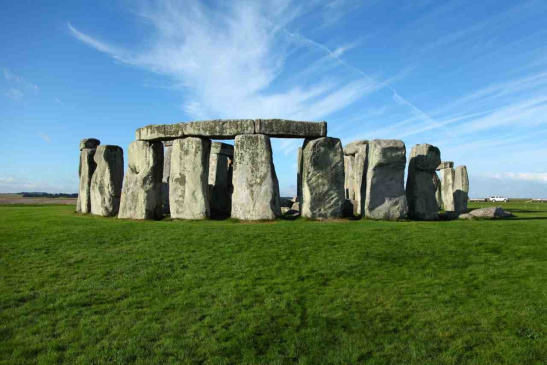
\includegraphics[width=\paperwidth,height=\paperheight]{Imagens/stonerange.jpg}
	}
	
	% Frame 3: plano de fundo
	\begin{frame}
	\frametitle{\textcolor{yellow}{Mudança das Estações}}
	%\flushbottom\color{yellow}{\normalsize Changing seasons}
	
\end{frame}
}

{%
\usebackgroundtemplate{
	\centering
	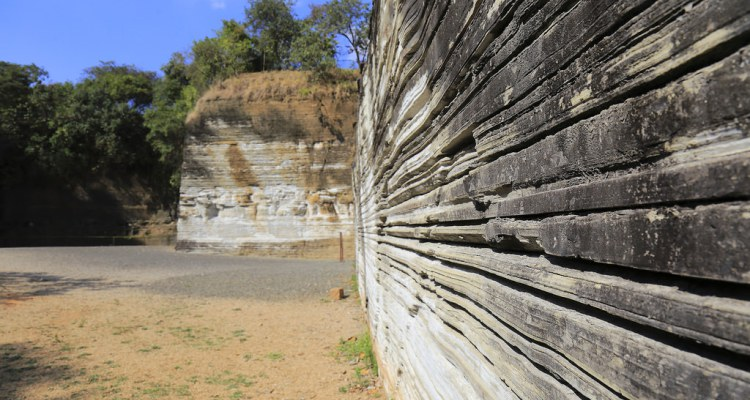
\includegraphics[width=\paperwidth,height=\paperheight]{Imagens/varvite.jpg}
}

% Frame 3: plano de fundo
\begin{frame}
\frametitle{\textcolor{yellow}{Varvito (Itu - São Paulo)}}
%\flushbottom\color{yellow}{\normalsize Changing seasons}

\end{frame}
}

%%%%%%%%%%%%%%%%%%%%%%%%%%%%%%%%%%%%%%%%%%%%%%%%%%%%%%%%%%%%%%%%%%%%%%%%%%%%%%%%%%%%%%%%%%%%%
\subsection{Definições}

\begin{frame}
	\frametitle{Definições}
	\begin{columns}
		\column{0.55\textwidth}
		\footnotesize
		\justifying
		\begin{itemize}
			\item[Inteligência Artificial:] todo programa computacional que tem a capacidade de melhorar a si mesmo por meio da experiência.
			\pause
			\item[Grupos de IA:]
			\begin{enumerate}
				{\tiny 
					\item  Redes Neuronais Artificiais \citep{Minsky1969,Michie1994,MacKay2005};
					\item Árvores de Decisão \citep{Mitchell1997,Simard2000,Roberts2002};
					\item Classificadores Estatísticos \citep{Michel2016};
					\item Mapas auto-organizados \citep{Kohonen1989,Haykin1999};
				}
			\end{enumerate}
			\pause
			\item[Classificadores:] usam o conceito de distância no espaço de atributos;
			\pause
			\item[C. Euclideano:] calcula um centroide no espaço de atributos.
			\pause
			\item[C. de Mahalanobis:] leva em consideração a forma do agrupamento.
			\pause
			\item[Mapas auto-organizados:] inspirados funcionamento do córtex neuronal são baseados em um grafo orientado que funciona como uma rede interconectada. 
		\end{itemize}
	\end{columns}
\end{frame}


\subsection{Pesquisa bibliográfica}

\begin{frame}
\frametitle{Um breve histórico sobre as redes neuronais artificiais}
\pause
\begin{small}
\smartdiagram[flow diagram:horizontal]{\textcolor{blue}{\cite{McCulloch1943}}}
\end{small}
\begin{itemize}
\item Definem o a função do neurônio numérico cuja a resposta dependia da entrada dos dados da rede e dos pesos utilizados e a denominam como Perceptron.
\end{itemize}	
\end{frame}


\begin{frame}
\frametitle{Um breve histórico sobre as redes neuronais artificiais.}
\begin{small}
\smartdiagram[flow diagram:horizontal]{\citet{McCulloch1943}, \textcolor{blue}{\citet{Rosenblatt1962}}}
\end{small}
\begin{itemize}
\item Definem teoria de convergência do Perceptron onde ele prova que modelos de neurônios possuem propriedades similares ao cérebro humano.
\end{itemize}
\end{frame}

\begin{frame}
\frametitle{Um breve histórico sobre as redes neuronais artificiais}
\begin{small}
\smartdiagram[flow diagram:horizontal]{\citet{McCulloch1943}, \citet{Rosenblatt1962}, \textcolor{blue}{\cite{Minsky1969}}}
\end{small}
\begin{itemize}
\item Demonstraram que Perceptrons somente resolvem uma classe muito limitada de problemas que podem ser linearizados.
\end{itemize}
\end{frame}

\begin{frame}
\frametitle{Um breve histórico sobre as redes neuronais artificiais}
\begin{small}
\smartdiagram[flow diagram:horizontal]{\citet{McCulloch1943}, \citet{Rosenblatt1962}, \cite{Minsky1969}, \textcolor{blue}{\cite{Hopfield1982}}}
\end{small}
\begin{itemize}
\item Resolve problemas não-lineares criando um  modelo de memória auto-associativa com a habilidade de armazenar e depois recuperar um certo conjunto de padrões do dado.  
%\item The collective properties of this model produce a content-addressable memory which correctly yields an entire	memory from any subpart of sufficient size.
\end{itemize}
\end{frame}

\begin{frame}
\frametitle{Um breve histórico sobre as redes neuronais artificiais}
\begin{small}
\smartdiagram[flow diagram:horizontal]{\citet{Rosenblatt1962}, \cite{Minsky1969}, \cite{Hopfield1982}, \textcolor{blue}{\cite{Kohonen1989}}}
\end{small}
\begin{itemize}
\item Cria uma ferramenta eficiente para a identificação de padrões multivariados.  
%\item The collective properties of this model produce a content-addressable memory which correctly yields an entire	memory from any subpart of sufficient size.
\end{itemize}
\end{frame}

\begin{frame}
\frametitle{Estado da arte}
\framesubtitle{na geofísica}
\begin{itemize}
\item Primeira fase \textcolor{red}{entre 1988 e 1994}: descobrir o que as redes neuronais podem fazer. 
\pause
\item Segunda fase \textcolor{red}{entre 1995 até o presente}:integrar o resultado da RNA com outros resultados.
\end{itemize}

\begin{flushleft}
\citep{Poulton2002, Artero2009}
\end{flushleft}

\end{frame}

\begin{frame}
\frametitle{Estado da arte}
\framesubtitle{na perfilagem de poços}
\begin{small}
\smartdiagram[flow diagram:horizontal]{\textcolor{blue}{\cite{Zhang1999}}}
\end{small}
\begin{itemize}
\item Algoritmos baseados em derivadas nas curvas de log não identificam camadas muito finas, ou ruído.
\end{itemize}
\end{frame}

\begin{frame}
\frametitle{Estado da arte}
\framesubtitle{na perfilagem de poços}
\begin{small}
\smartdiagram[flow diagram:horizontal]{\cite{Zhang1999},\textcolor{blue}{\cite{Chakravarthy1999}}}
\end{small}
%\pause
\begin{itemize}
\item consegue através do uso da função radial localizar os limites de camadas em alta definição em dados de log de indução (HDIL).
\end{itemize}
\end{frame}

\begin{frame}
\frametitle{Estado da arte}
\framesubtitle{na perfilagem de poços}
\begin{small}
\smartdiagram[flow diagram:horizontal]{\cite{Zhang1999},\cite{Chakravarthy1999}, \textcolor{blue}{\cite{Benaouda1999}}}
\end{small}
%\pause
\begin{itemize}
\item consegue classificar tipos litológicos em poços parcialmente desmoronados.
\end{itemize}
\end{frame}

\begin{frame}
\frametitle{Estado da arte}
\framesubtitle{na perfilagem de poços}
\begin{small}
\smartdiagram[flow diagram:horizontal]{\cite{Zhang1999},\cite{Chakravarthy1999}, \cite{Benaouda1999}, \textcolor{blue}{\cite{Saljooghi2014}}}
\end{small}
%\pause
\begin{itemize}
\item topo e base de camadas que podem ser associadas com mudanças das propriedades petrofísicas. 
\end{itemize}
\end{frame}

\begin{frame}
\frametitle{Estado da arte}
\framesubtitle{na perfilagem de poços}
\begin{small}
\smartdiagram[flow diagram:horizontal]{\cite{Chakravarthy1999}, \cite{Benaouda1999},\cite{Saljooghi2014}, \textcolor{blue}{\cite{Gloaguen2017}} }
\end{small}
%\pause
\begin{itemize}
\item Chama a atenção para importância relativa das propriedades físicas no \textit{output} da rede neuronal. 
\end{itemize}
\end{frame}

\subsection{Objetivo}

\begin{frame}
	\frametitle{Objetivo}
	\begin{columns}\footnotesize 
		\justifying
		\column{0.55\textwidth}
		\begin{itemize}
			\item[Problema Geofísico:] Identificação de rochas em dados de perfilagem da Bacia do Paraná nos termos de inteligência artificial;
			\pause
			\item[Maneira de resolver:] utilizando um mapa auto-organizado (SOM)  e dois classificadores estatísticos e escolher o melhor destes para aplicar no dado real;
			\pause
			\item[Estratégia:] Comparar o resultado dos três métodos em dados sintéticos, Kohonen (SOM),  e os classificadores euclideanos e de mahalanobis. E aplicar a melhor metodologia aos dados reais. 
		\end{itemize}
	\end{columns}
\end{frame}




%%%%%%%%%%%%%%%%%%%%%%%%%%%%%%%%%%%%%%%%%%%%%%%%%%%%%%%%%%%%%%%%%%%%%%%%%%%%
%---------------------------------CONTEXTO GEOLÓGICO------------------------------------
%%%%%%%%%%%%%%%%%%%%%%%%%%%%%%%%%%%%%%%%%%%%%%%%%%%%%%%%%%%%%%%%%%%%%%%%%%%%

\section{Contexto Geológico e Localização}
\begin{frame}[<+->]
\frametitle{Contexto Geológico}
\transboxin%efeito de transição	
\begin{itemize}
\justifying

\item Localização: Centro-sul; 		
\item Extensão: $1.100.000$ $Km^{2}$ \cite{Schneider_1974,zalan_p._v._tectonica_1987};
\item Idade: Cambriano ao Quaternário com embasamento pré-cambriano\\ \cite{Schneider_1974,boletim_2007};
\item Classificação: Bacia de sinéclise ou cratônica marginal, sob domínio flexural de crosta \cite{cordani_1984,borghi_2002}; 
\item Depocentro: $7000$ m aproximadamente \cite{milani_outline_1999};
\end{itemize}			
\end{frame}

%-----------------------------------Estratigrafia----------------------------------

%########## 1 ###########
\begin{frame}
\frametitle{Contexto Geológico}
\begin{columns}


\begin{column}{0.4\textwidth}
\begin{figure}
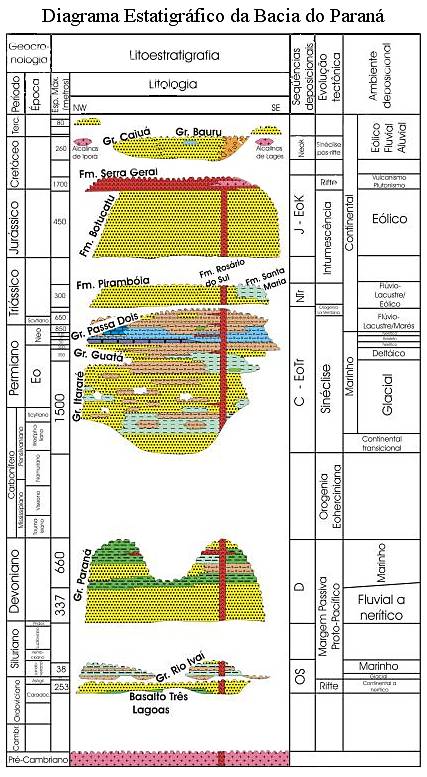
\includegraphics[scale=0.4]{Imagens/diagrama.png}
\end{figure}
\end{column}

\begin{column}{0.55\textwidth}
\begin{block}{As $6$ supersequências}
Bauru $\Longleftrightarrow$  sequência neocretácea\\
Gondwana III $\Longleftrightarrow$ sequência jurássica-eocretácea\\
Gondwana II $\Longleftrightarrow$ sequência neotriássica \\
Gondwana I $\Longleftrightarrow$ sequência carbonífera-permiana\\ 
Paraná $\Longleftrightarrow$ sequência devoniana\\
Rio Ivaí $\Longleftrightarrow$ sequência ordovício-siluriana\\
\cite{Vail_1977,assine_1994,milani_orogenias_1998}
\end{block}

\end{column}


\end{columns}
\end{frame}	

%########## 2 ###########
\begin{frame}
\frametitle{Contexto Geológico}
\begin{columns}
\begin{column}{0.4\textwidth}
\begin{figure}
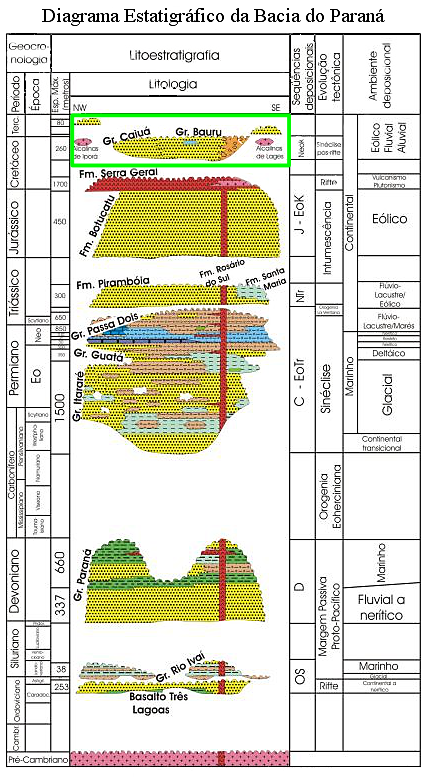
\includegraphics[scale=0.36]{Imagens/diagramabauru.png}
\end{figure}
\end{column}
\begin{column}{0.55\textwidth}
\begin{block}{As $6$ supersequências}
\textcolor{green}{Bauru $\Longleftrightarrow$  sequência neocretácea}\\
Gondwana III $\Longleftrightarrow$ sequência jurássica-eocretácea\\
Gondwana II $\Longleftrightarrow$ sequência neotriássica \\
Gondwana I $\Longleftrightarrow$ sequência carbonífera-permiana\\ 
Paraná $\Longleftrightarrow$ sequência devoniana\\
Rio Ivaí $\Longleftrightarrow$ sequência ordovício-siluriana\\
\cite{Vail_1977,assine_1994,milani_orogenias_1998}
\end{block}
\end{column}
\end{columns}
\end{frame}	

%########## 3 ###########
\begin{frame}
\frametitle{Contexto Geológico}
\begin{columns}
\begin{column}{0.4\textwidth}
\begin{figure}
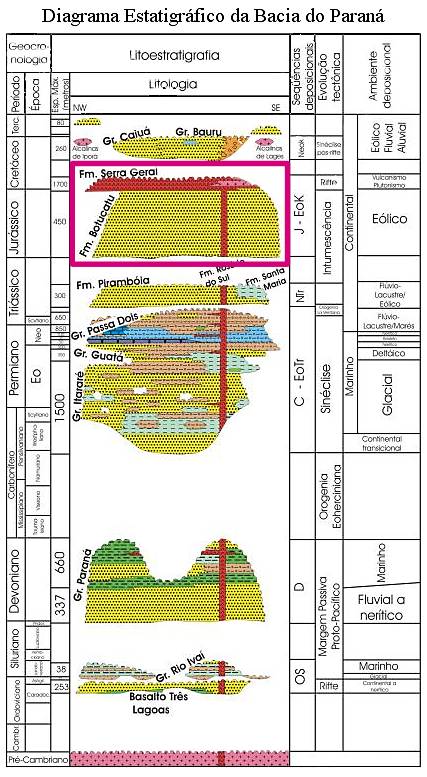
\includegraphics[scale=0.36]{Imagens/diagramagondwanaiii.png}
\end{figure}
\end{column}
\begin{column}{0.55\textwidth}
\begin{block}{As $6$ supersequências}
Bauru $\Longleftrightarrow$  sequência neocretácea.\\
\textcolor{purple}{Gondwana III $\Longleftrightarrow$ sequência jurássica-eocretácea}\\
Gondwana II $\Longleftrightarrow$ sequência neotriássica \\
Gondwana I $\Longleftrightarrow$ sequência carbonífera-permiana\\ 
Paraná $\Longleftrightarrow$ sequência devoniana\\
Rio Ivaí $\Longleftrightarrow$ sequência ordovício-siluriana\\
\cite{Vail_1977,assine_1994,milani_orogenias_1998}
\end{block}
\end{column}
\end{columns}
\end{frame}

%########## 4 ###########
\begin{frame}
\frametitle{Contexto Geológico}
\begin{columns}
\begin{column}{0.4\textwidth}
\begin{figure}
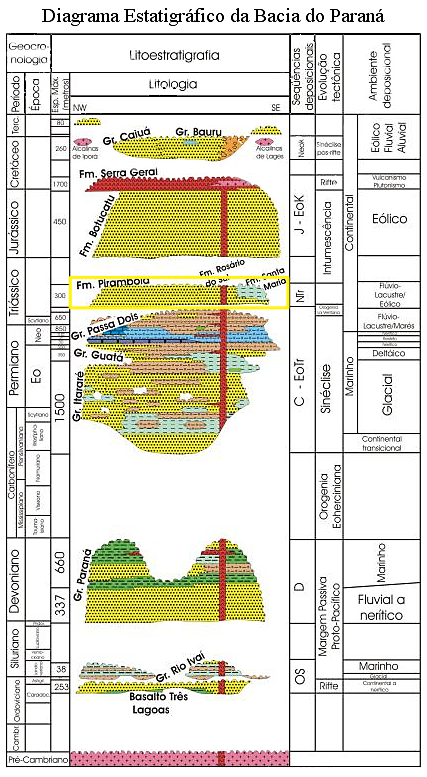
\includegraphics[scale=0.36]{Imagens/diagramagondwanaii.png}
\end{figure}
\end{column}
\begin{column}{0.55\textwidth}
\begin{block}{As $6$ supersequências}
Bauru $\Longleftrightarrow$  sequência neocretácea.\\
Gondwana III $\Longleftrightarrow$ sequência jurássica-eocretácea\\
\textcolor{yellow}{Gondwana II $\Longleftrightarrow$ sequência neotriássica} \\
Gondwana I $\Longleftrightarrow$ sequência carbonífera-permiana\\ 
Paraná $\Longleftrightarrow$ sequência devoniana\\
Rio Ivaí $\Longleftrightarrow$ sequência ordovício-siluriana\\
\cite{Vail_1977,assine_1994,milani_orogenias_1998}
\end{block}
\end{column}
\end{columns}
\end{frame}

%########## 5 ###########
\begin{frame}
\frametitle{Contexto Geológico}
\begin{columns}
\begin{column}{0.4\textwidth}
\begin{figure}
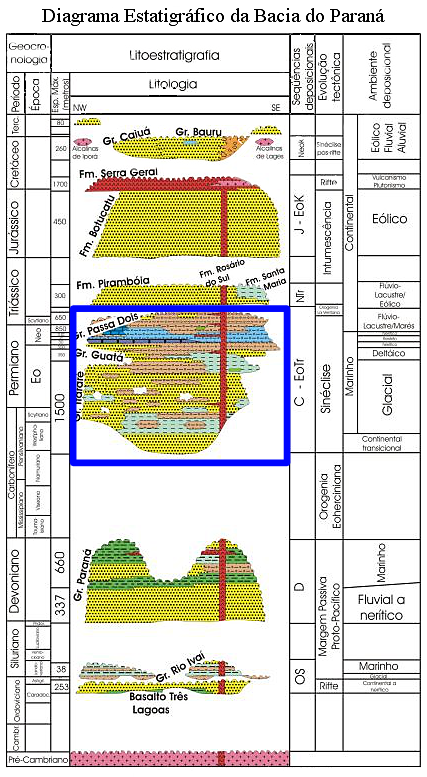
\includegraphics[scale=0.36]{Imagens/diagramagondwanai.png}
\end{figure}
\end{column}
\begin{column}{0.55\textwidth}
\begin{block}{As $6$ supersequências}

Bauru $\Longleftrightarrow$  sequência neocretácea.\\
Gondwana III $\Longleftrightarrow$ sequência jurássica-eocretácea\\
Gondwana II $\Longleftrightarrow$ sequência neotriássica \\
\textcolor{blue}{Gondwana I $\Longleftrightarrow$ sequência carbonífera-permiana}\\ 
Paraná $\Longleftrightarrow$ sequência devoniana\\
Rio Ivaí $\Longleftrightarrow$ sequência ordovício-siluriana\\
\cite{Vail_1977,assine_1994,milani_orogenias_1998}
\end{block}
\end{column}
\end{columns}
\end{frame}

%########## 6 ###########
\begin{frame}
\frametitle{Contexto Geológico}
\begin{columns}
\begin{column}{0.4\textwidth}
\begin{figure}
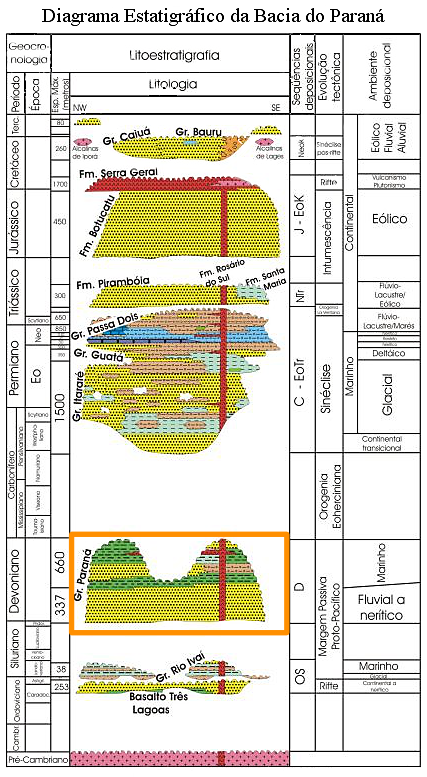
\includegraphics[scale=0.36]{Imagens/diagramaparana.png}
\end{figure}
\end{column}
\begin{column}{0.55\textwidth}
\begin{block}{As $6$ supersequências}
Bauru $\Longleftrightarrow$  sequência neocretácea.\\
Gondwana III $\Longleftrightarrow$ sequência jurássica-eocretácea\\
Gondwana II $\Longleftrightarrow$ sequência neotriássica \\
Gondwana I $\Longleftrightarrow$ sequência carbonífera-permiana\\ 
\textcolor{orange}{Paraná $\Longleftrightarrow$ sequência devoniana}\\
Rio Ivaí $\Longleftrightarrow$ sequência ordovício-siluriana\\
\cite{Vail_1977,assine_1994,milani_orogenias_1998}
\end{block}
\end{column}
\end{columns}
\end{frame}

%########## 7 ###########
\begin{frame}
\frametitle{Contexto Geológico}
\begin{columns}
\begin{column}{0.4\textwidth}
\begin{figure}
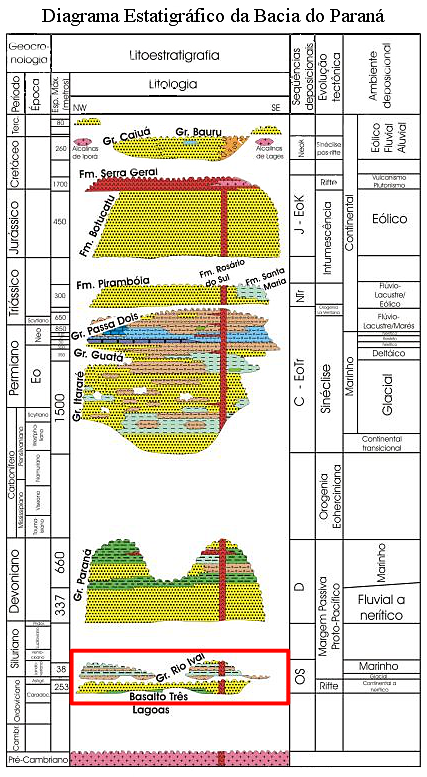
\includegraphics[scale=0.36]{Imagens/diagramarioivai.png}
\end{figure}
\end{column}
\begin{column}{0.55\textwidth}
\begin{block}{As $6$ supersequências}
Bauru $\Longleftrightarrow$  sequência neocretácea.\\
Gondwana III $\Longleftrightarrow$ sequência jurássica-eocretácea\\
Gondwana II $\Longleftrightarrow$ sequência neotriássica \\
Gondwana I $\Longleftrightarrow$ sequência carbonífera-permiana\\ 
Paraná $\Longleftrightarrow$ sequência devoniana\\
\textcolor{red}{Rio Ivaí $\Longleftrightarrow$ sequência ordovício-siluriana}\\
\cite{Vail_1977,assine_1994,milani_orogenias_1998}
\end{block}
\end{column}
\end{columns}
\end{frame}


\begin{frame}
\frametitle{Localização e extensão da Bacia Sedimentar}
\begin{figure}[H]
\centering
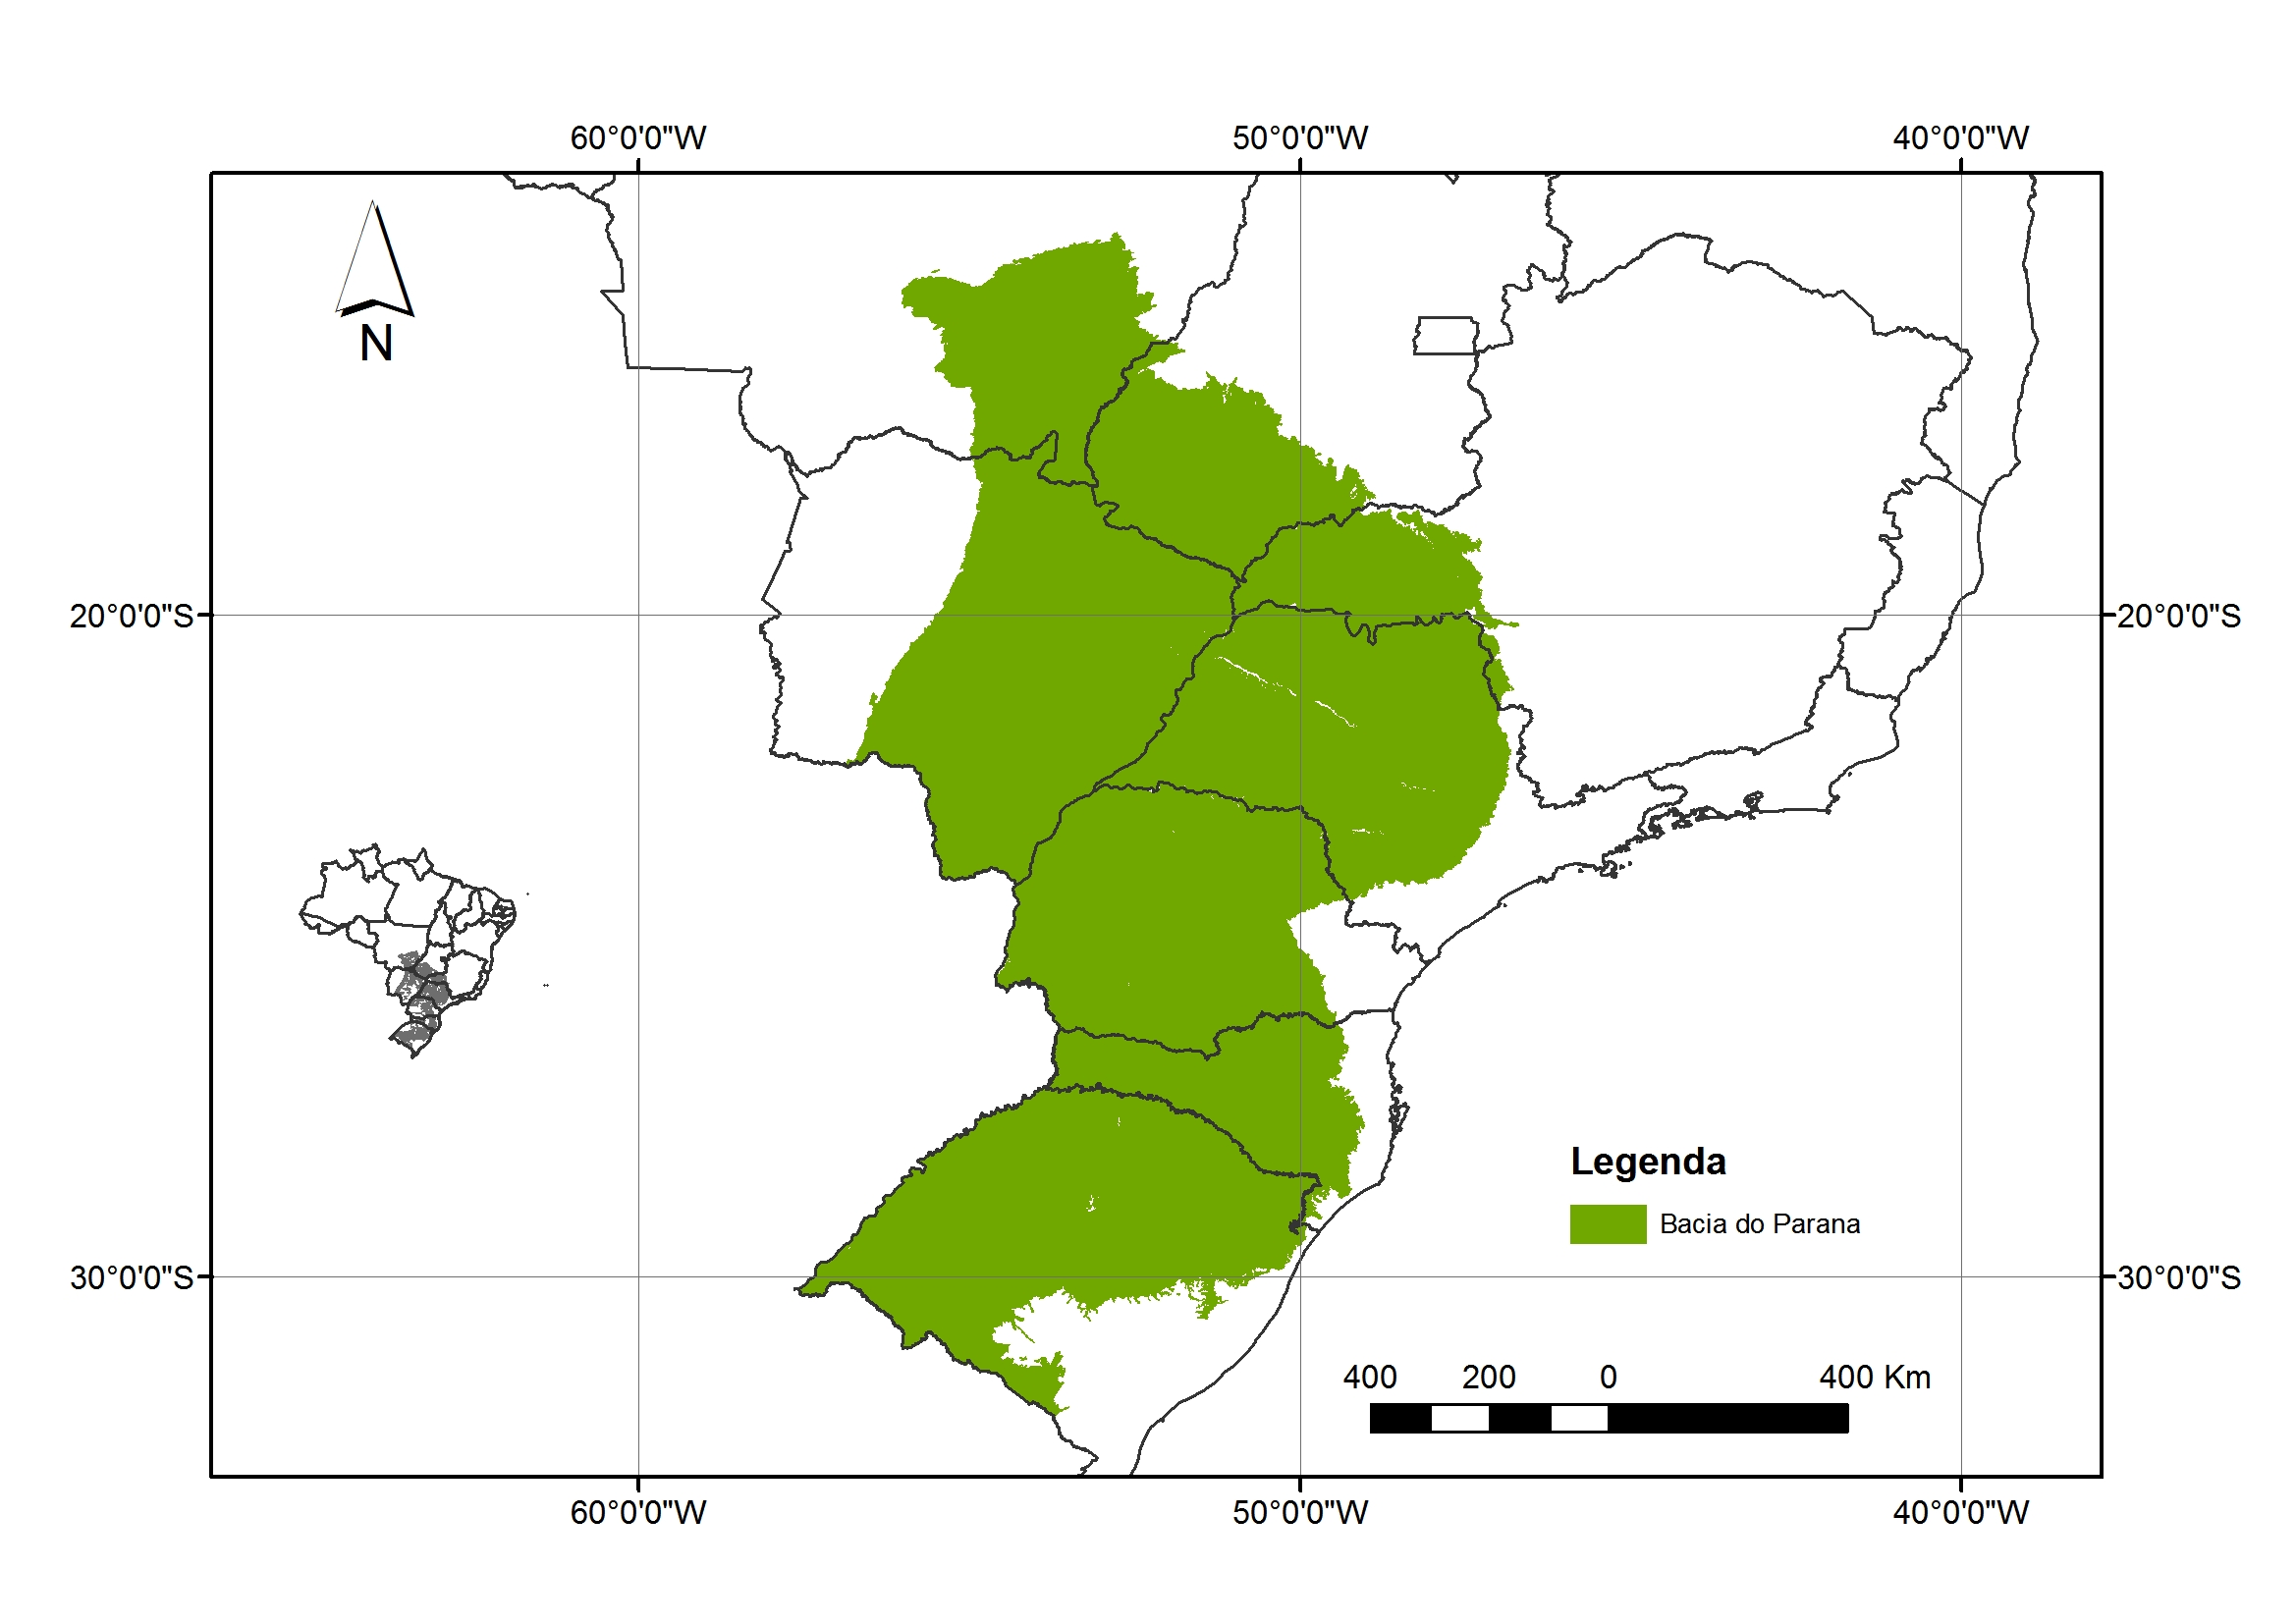
\includegraphics[scale=0.3]{Imagens/BaciaParana.jpg}
\caption{Mapa de localização da Bacia do Paraná. }
\label{mapa geologico}
\end{figure}
\end{frame}





%%%%%%%%%%%%%%%%%%%%%%%%%%%%%%%%%%%%%%%%%%%%%%%%%%%%%%%%%%%%%%%%%%%%%%%%%%%%
%-------------------------OBJETIVO------------------------------
%%%%%%%%%%%%%%%%%%%%%%%%%%%%%%%%%%%%%%%%%%%%%%%%%%%%%%%%%%%%%%%%%%%%%%%%%%%%










%%%%%%%%%%%%%%%%%%%%%%%%%%%%%%%%%%%%%%%%%%%%%%%%%%%%%%%%%%%%%%%%%%%%%%%%%%%%
%---------------------------NATUREZA DO DADO--------------------------
%%%%%%%%%%%%%%%%%%%%%%%%%%%%%%%%%%%%%%%%%%%%%%%%%%%%%%%%%%%%%%%%%%%%%%%%%%%%



%\begin{frame}
%	\frametitle{Modelo proposto}
% \begin{scriptsize}
%	\begin{table}[H]
%		\centering
%		\caption{Compilação de propriedades físicas usadas para inferência de litologia \citep{Telford_1993}.}
%		\label{rock-properties1}
%			\begin{tabular}{@{}llllllllll@{}}
%				\toprule
%				Rocha         & Densidade ($g/cm^{3}$) & Raios-Gama ($Ci/g$)& Potencial-Espontâneo ($mV$)&   \\ \midrule
%				Conglomerado &     $2,50$  &       ---        &    ---        &      \\
%				Arenito  &    $2,35$      &       $2,00\leftrightarrow4,00$       &     ---       &      \\
%				Folhelho &   $2,40$       &      ---        &      ---      &    \\
%				Argilito &     $2,55$   &          ---     &       ---     &     \\
%				Siltito  &      $2,21$    &          ---     &       ---     &   \\
%				Dolomita &     $2,70$    &        $8,00$       &   ---         &       \\
%				Marga  &    $2,50$     &         ---      &    ---        &     \\
%				Basalto  &     $2,99$    &          $0,50$     &    ---       &      \\
%				Diabásio &    $2,90$    &         ---      &       ---     &     \\
%				Lava &     $2,61$    &      $0,33$         &      ---      &      \\
%				Granito &    $2,64$      &       $0,70\leftrightarrow4,80$        &      ---      &      \\
%				Gabro &    $3,03$     &       ---        &     ---       &       \\
%				Peridotito &   $3,15$    &      ---         &     ---       &      \\
%				Quartzito &    $2,60$    &        $5,00$      &     ---       &    \\
%				Xisto &   $2,64$    &         ---      &      ---      &    \\
%				Gnaisse &    $2,80$     &      ---         &    ---        &        \\
%				Serpentinito &    $2,78$     &   ---            &   ---     &        \\
%				Anfibolito &  $2,96$       &          ---     &       ---     &        \\
%				Eclogito &  $3,37$    &       ---        &      ---      &    \\
%				Mármore &   $2,75$       &      ---         &     ---       &      \\ \bottomrule
%			\end{tabular}
%	\end{table}
%\end{scriptsize}
%\end{frame}
%
%\begin{frame}
%	\frametitle{Modelo proposto}
%	\begin{scriptsize}
%		\begin{table}[H]
%			\centering
%			\caption{Compilação de propriedades físcas usadas na inferência de porosidade, permeabilidade. \cite{Telford_1993}.}
%			\label{rock-properties2}
%			\begin{tabular}{@{}llllllllll@{}}
%				\toprule
%				Rocha   & Resistividade ($\Omega/m$) &  Neutrão ($API$) & Velocidade ($km/s$)  &    \\ \midrule
%				Conglomerado &    $2\times10^{3}\leftrightarrow10^{4}$       &    ---           &     $1,80\leftrightarrow4,90$       &     \\
%				Arenito  &    $1\leftrightarrow6,4\times10^{8}$       &      ---         &     $4,00\leftrightarrow4,30$       &   \\
%				Folhelho &     $50\leftrightarrow10^{7}$      &      ---         &      $2,15\leftrightarrow3,30$      &   \\
%				Argilito &     $10\leftrightarrow8\times10^{2}$      &       ---        &     ---       &      \\
%				Siltito  &      $1\leftrightarrow100$     &      ---         &         $4,00\leftrightarrow6,20$    &         \\
%				Dolomita &   $3,5\times10^{2}\leftrightarrow5\times10^{3}$        &    ---           &      $5,70\leftrightarrow6,00$      &      \\
%				Marga  &     $3\leftrightarrow70$      &     ---          &     ---       &     \\
%				Basalto  &     $10\leftrightarrow1,3\times10^{7}$      &     ---          &     $ 5,00\leftrightarrow5.80$         &     \\
%				Diabásio &  $20\leftrightarrow5\times10^{7}$         &      ---         &     ---       &  \\
%				Granito Porfirítico (seco) &     $1,3\times10^{6}$     &       ---        &     $5,80$       &    \\
%				Granito Porfirítico (úmido) &  $4,5\times10^{3}$          &      ---         &     $ 5,00\leftrightarrow5.60$         &      \\
%				Gabro &   $10^{3}\leftrightarrow10^{6}$       &      ---         &      $ 5,00\leftrightarrow5.80$        &     \\
%				Peridotito (seco) &   $6,5\times10^{3}$        &    ---           &       ---     &    \\
%				Peridotito (úmido) &    $3\times10^{3}$       &      ---         &      ---      &  \\
%				Xisto &    $20\leftrightarrow10^{4}$       &        ---       &       ---     &   \\
%				Gnaisse (seco) & $3\times10^{6}$          &         ---      &     ---       &   \\
%				Gnaisse (úmido) &   $6,8\times10^{4}$        &       ---        &      ---      &   \\
%				Tufa (seca) &      $2\times10^{3}$     &      ---         &     $1,80\leftrightarrow3,50$       &     \\
%				Tufa (úmida) &     $10^{5}$      &     ---          &     ---       &      \\
%				Mármore &  $10^{2}\leftrightarrow2,5\times10^{8}$         &       ---        &      ---      &    \\ \bottomrule
%			\end{tabular}
%		\end{table}
%	\end{scriptsize}
%\end{frame}

\section{Metodologia}

\begin{frame}
	\frametitle{Modelo proposto}
	\begin{figure}[H]
		\centering
		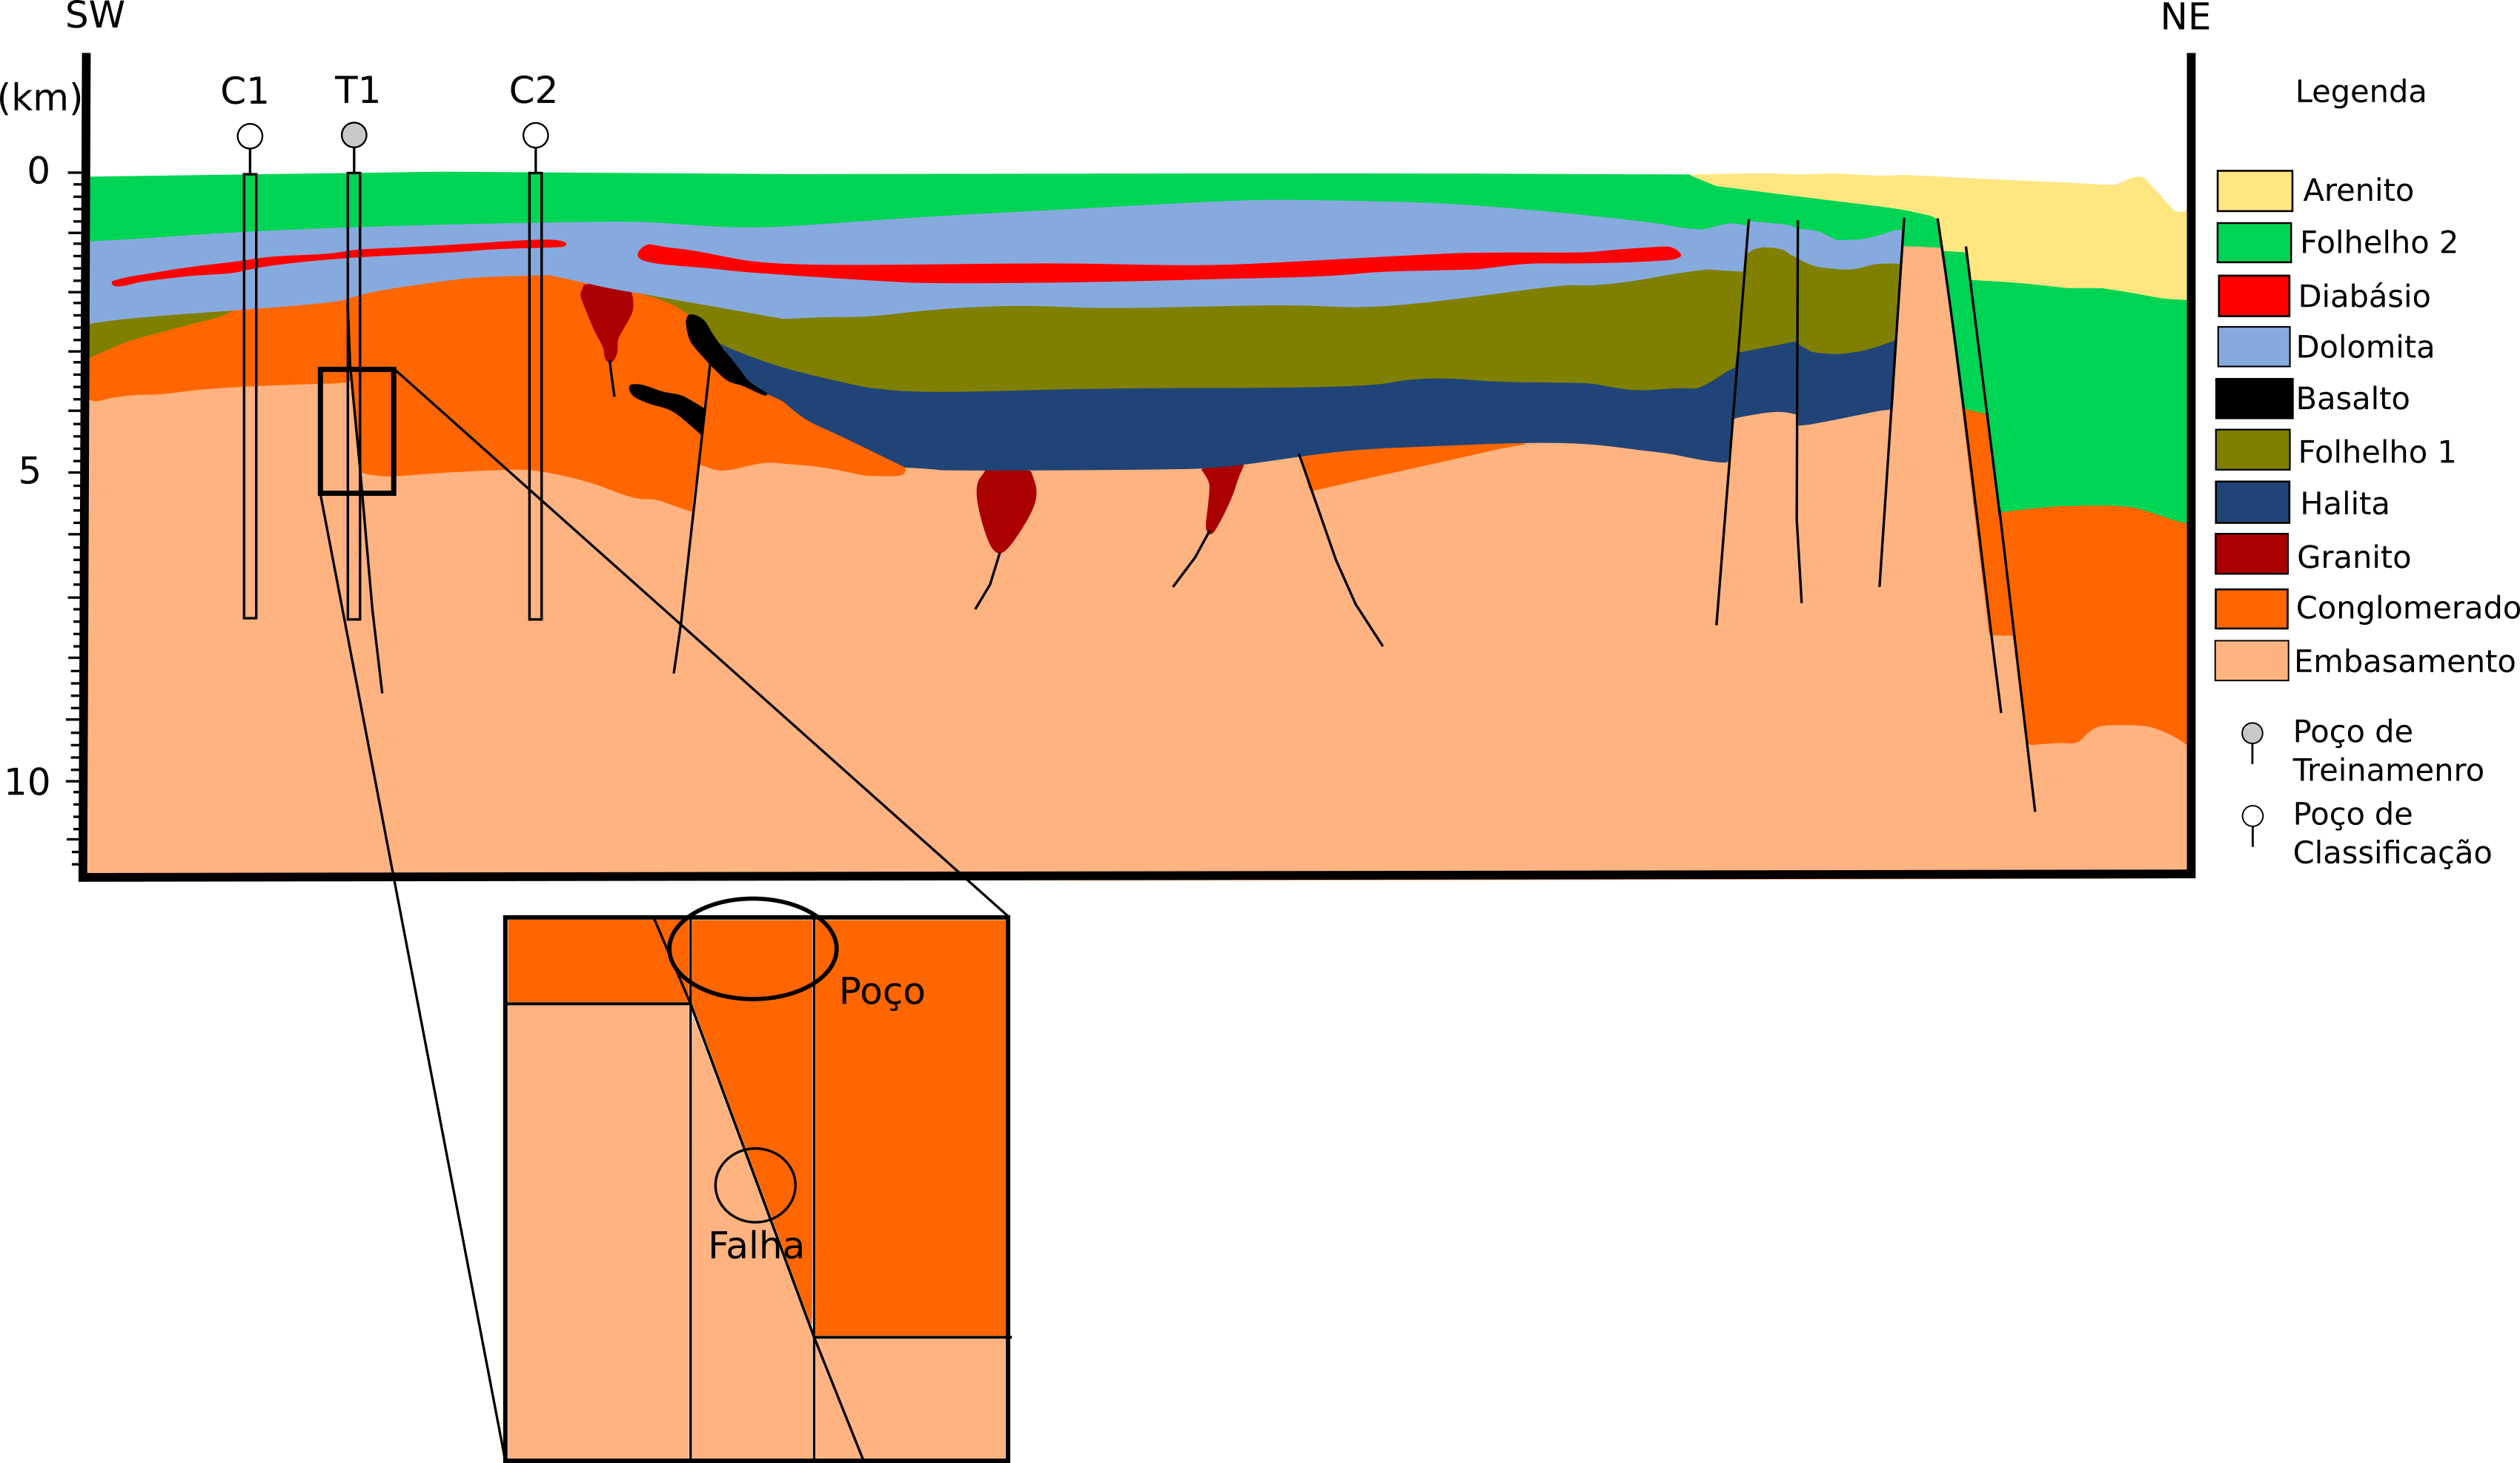
\includegraphics[scale=0.35]{Imagens/Modelo.png}
		\caption{Modelo Simplificado baseado em \cite{Sal2008}.}
		\label{modelo}
	\end{figure}
\end{frame}


\begin{frame}
\frametitle{Parâmetros do modelo}
\begin{table}[H]\tiny
	\caption{Propriedades físicas do modelo.}
	\begin{tabular}{@{}ccccccccccc@{}}
		\toprule
		Rocha & Densidade ($g/cm^{3}$) & Raio Gama ($Ci/g$) & Resistividade ($\Omega.m$)& Velocidade ($Km/s$) &\\ \midrule
		Conglomerado &     $2.30$ 		  &       $100.0$       &           $6000$           &			$2$   		   	&\\
		Folhelho	 &       $2.55$           &       $100.0$       &           $1000$           &     		$3$		 &\\
		Dolomita     &       $2.72$           &       $8.30$        &           $3.5 \times 10^{3}$           &  	$6$    			 &\\
		Diabásio    &       $2.91$           &       $30.0$        &           $15 \times 10^{7}$           &      $5.5$				 &\\
		Embasamento  &       $2.80$           &       $0.7$         &           $1.3 \times 10^{6}$           & 		$5$		     &\\ \bottomrule
	\end{tabular}
	
	\label{Tab1}
\end{table}
\begin{columns}
	\column{0.55\textwidth}
	\footnotesize
	\justifying
	\begin{itemize}\footnotesize
		\item[Taxa de amostragem:] $0.1$ observações/metro 
		\item[Contaminação:] $5$\% Ruído Gaussiano Randômico.
	\end{itemize}
\end{columns}
\end{frame}

\begin{frame}
\frametitle{Modelo proposto}
\framesubtitle{Descrição do modelo}
\begin{itemize}
\item modelo realístico com variação de $4$ propriedades físicas;
\pause
\item contaminação com $5\%$ ruído gaussiano;
\pause
\item taxa de amostragem $0,1$ dado/metro;
\pause
\item dados de propriedades previamente publicados quando encontrados.
\end{itemize}

\end{frame}

\begin{frame}
\frametitle{Modelo proposto}
\begin{figure}[H]
\centering
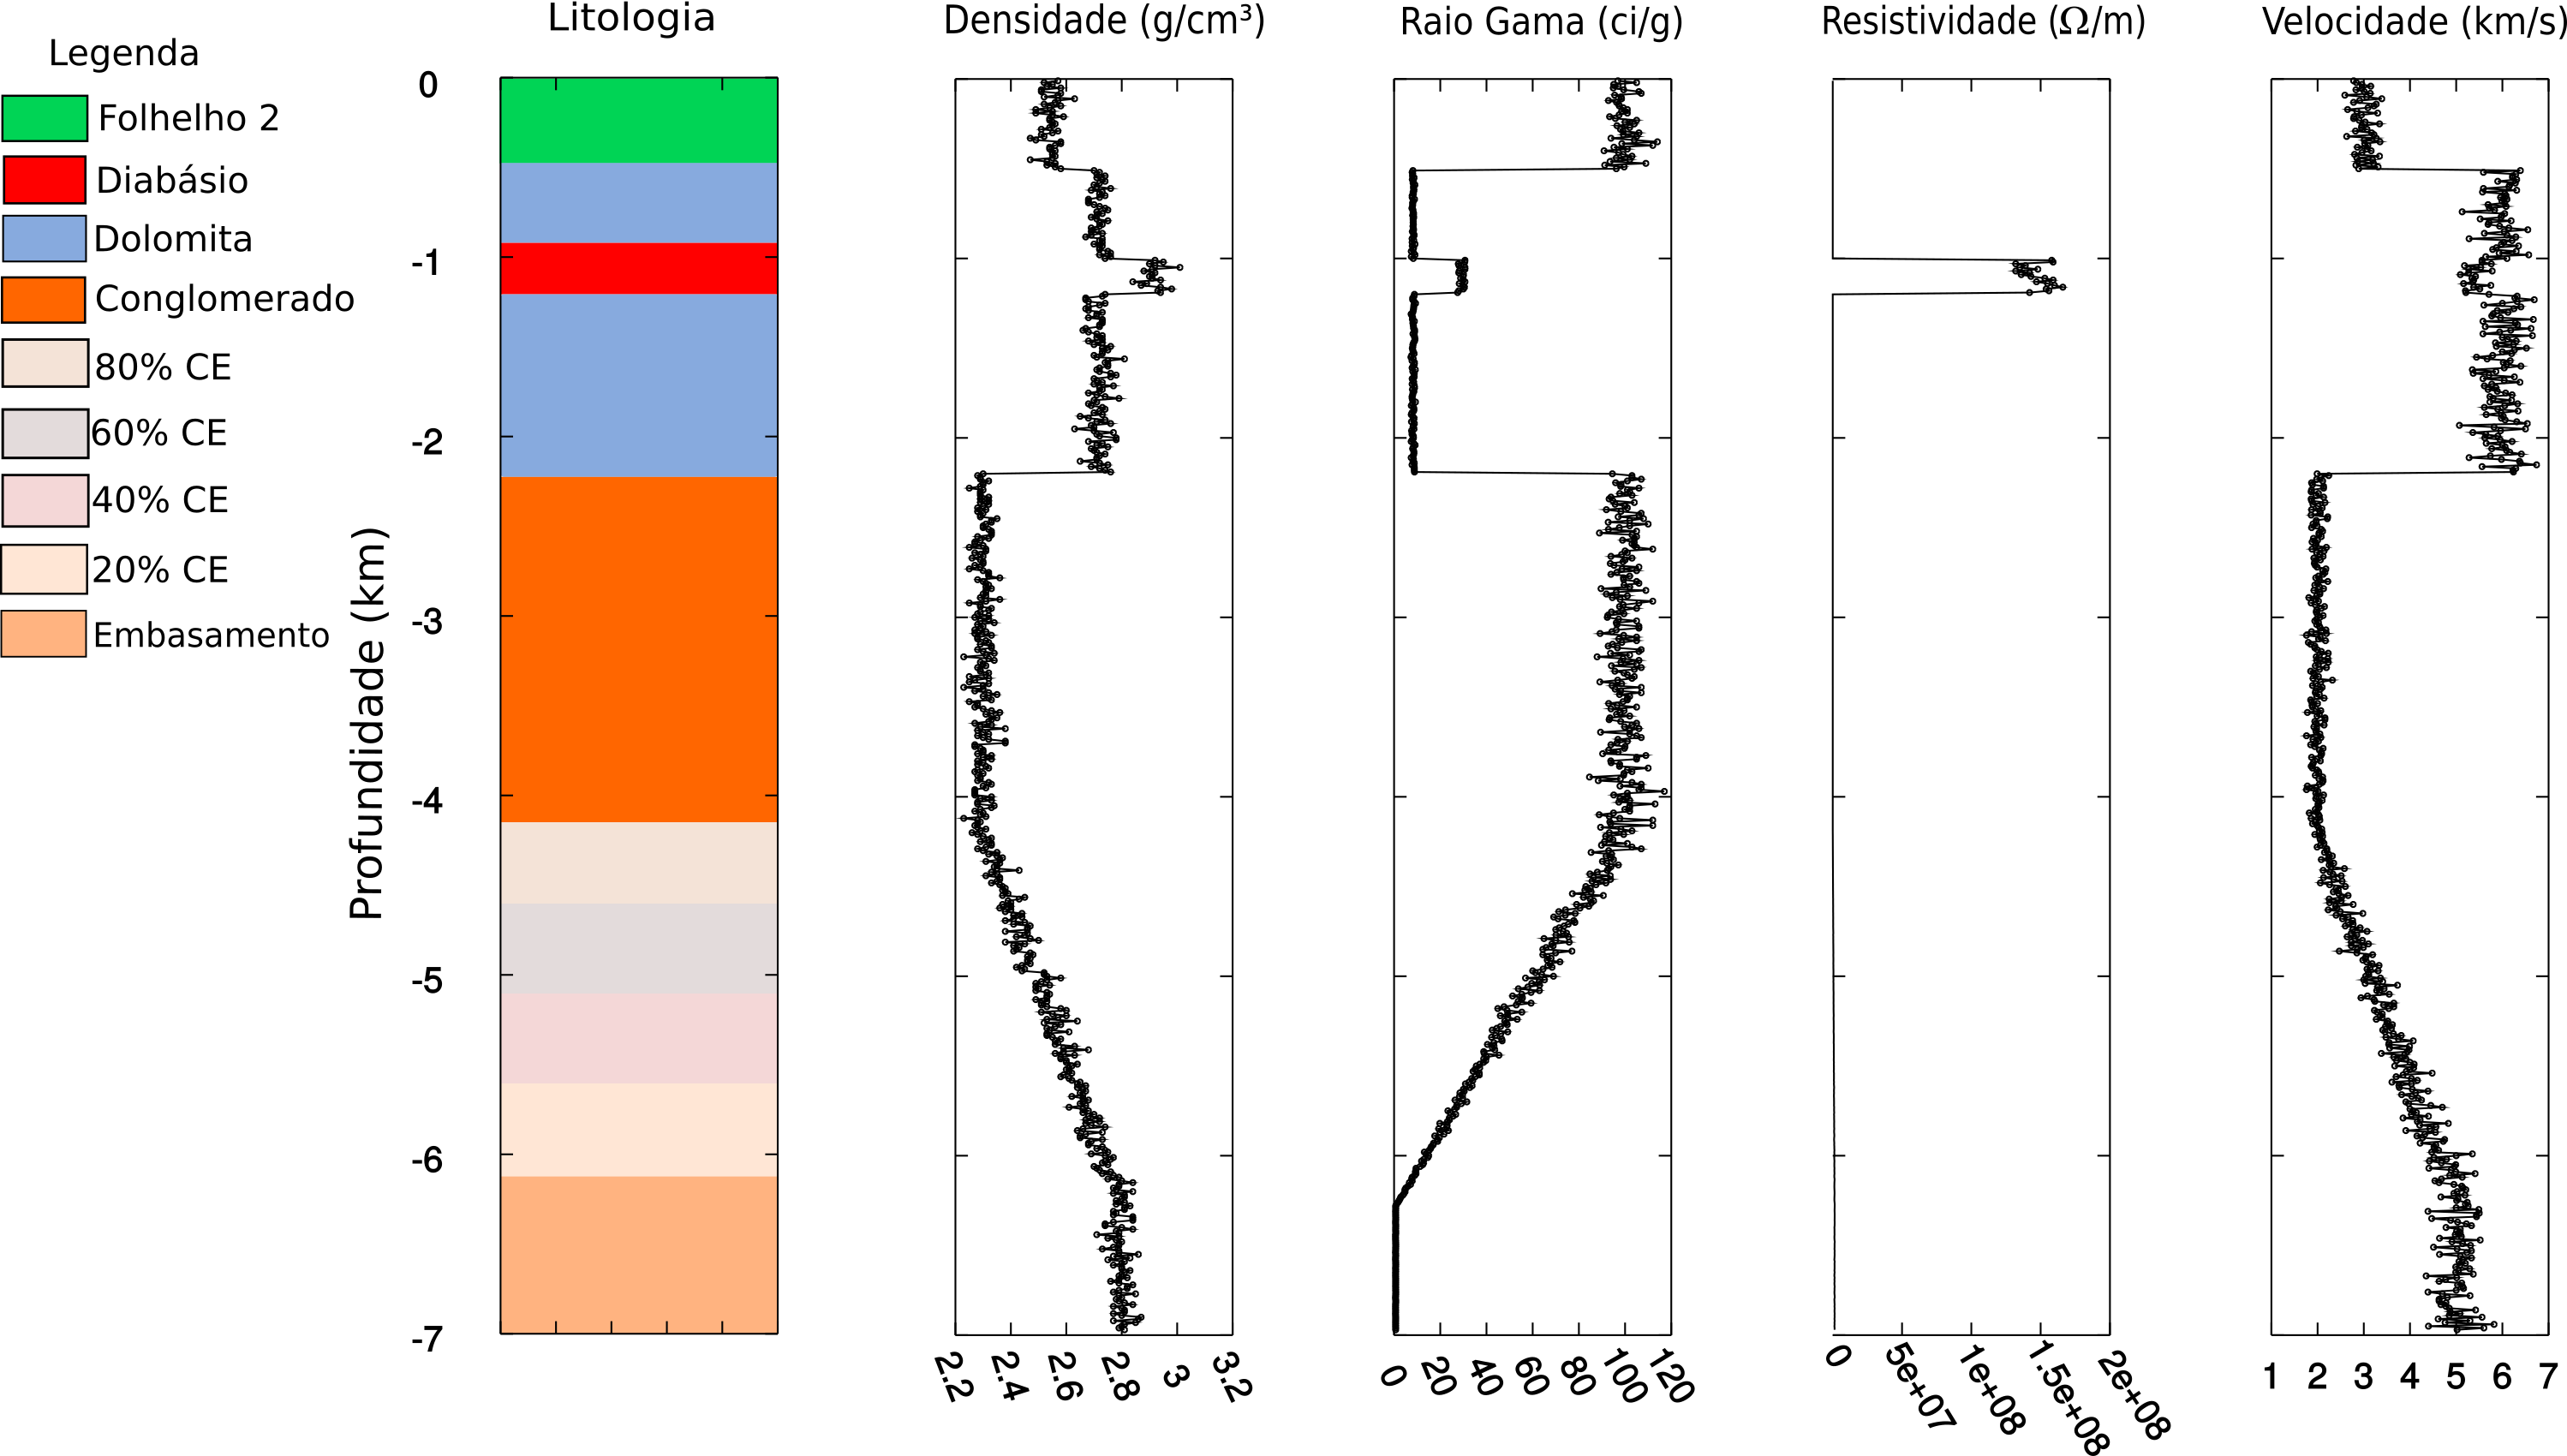
\includegraphics[scale=0.37]{Imagens/PocoT1.png}
\caption{Dado de perfilagem sintético, T1. }
\label{T1}
\end{figure}
\end{frame}


\begin{frame}
\frametitle{Modelo proposto}
\begin{figure}[H]
\centering
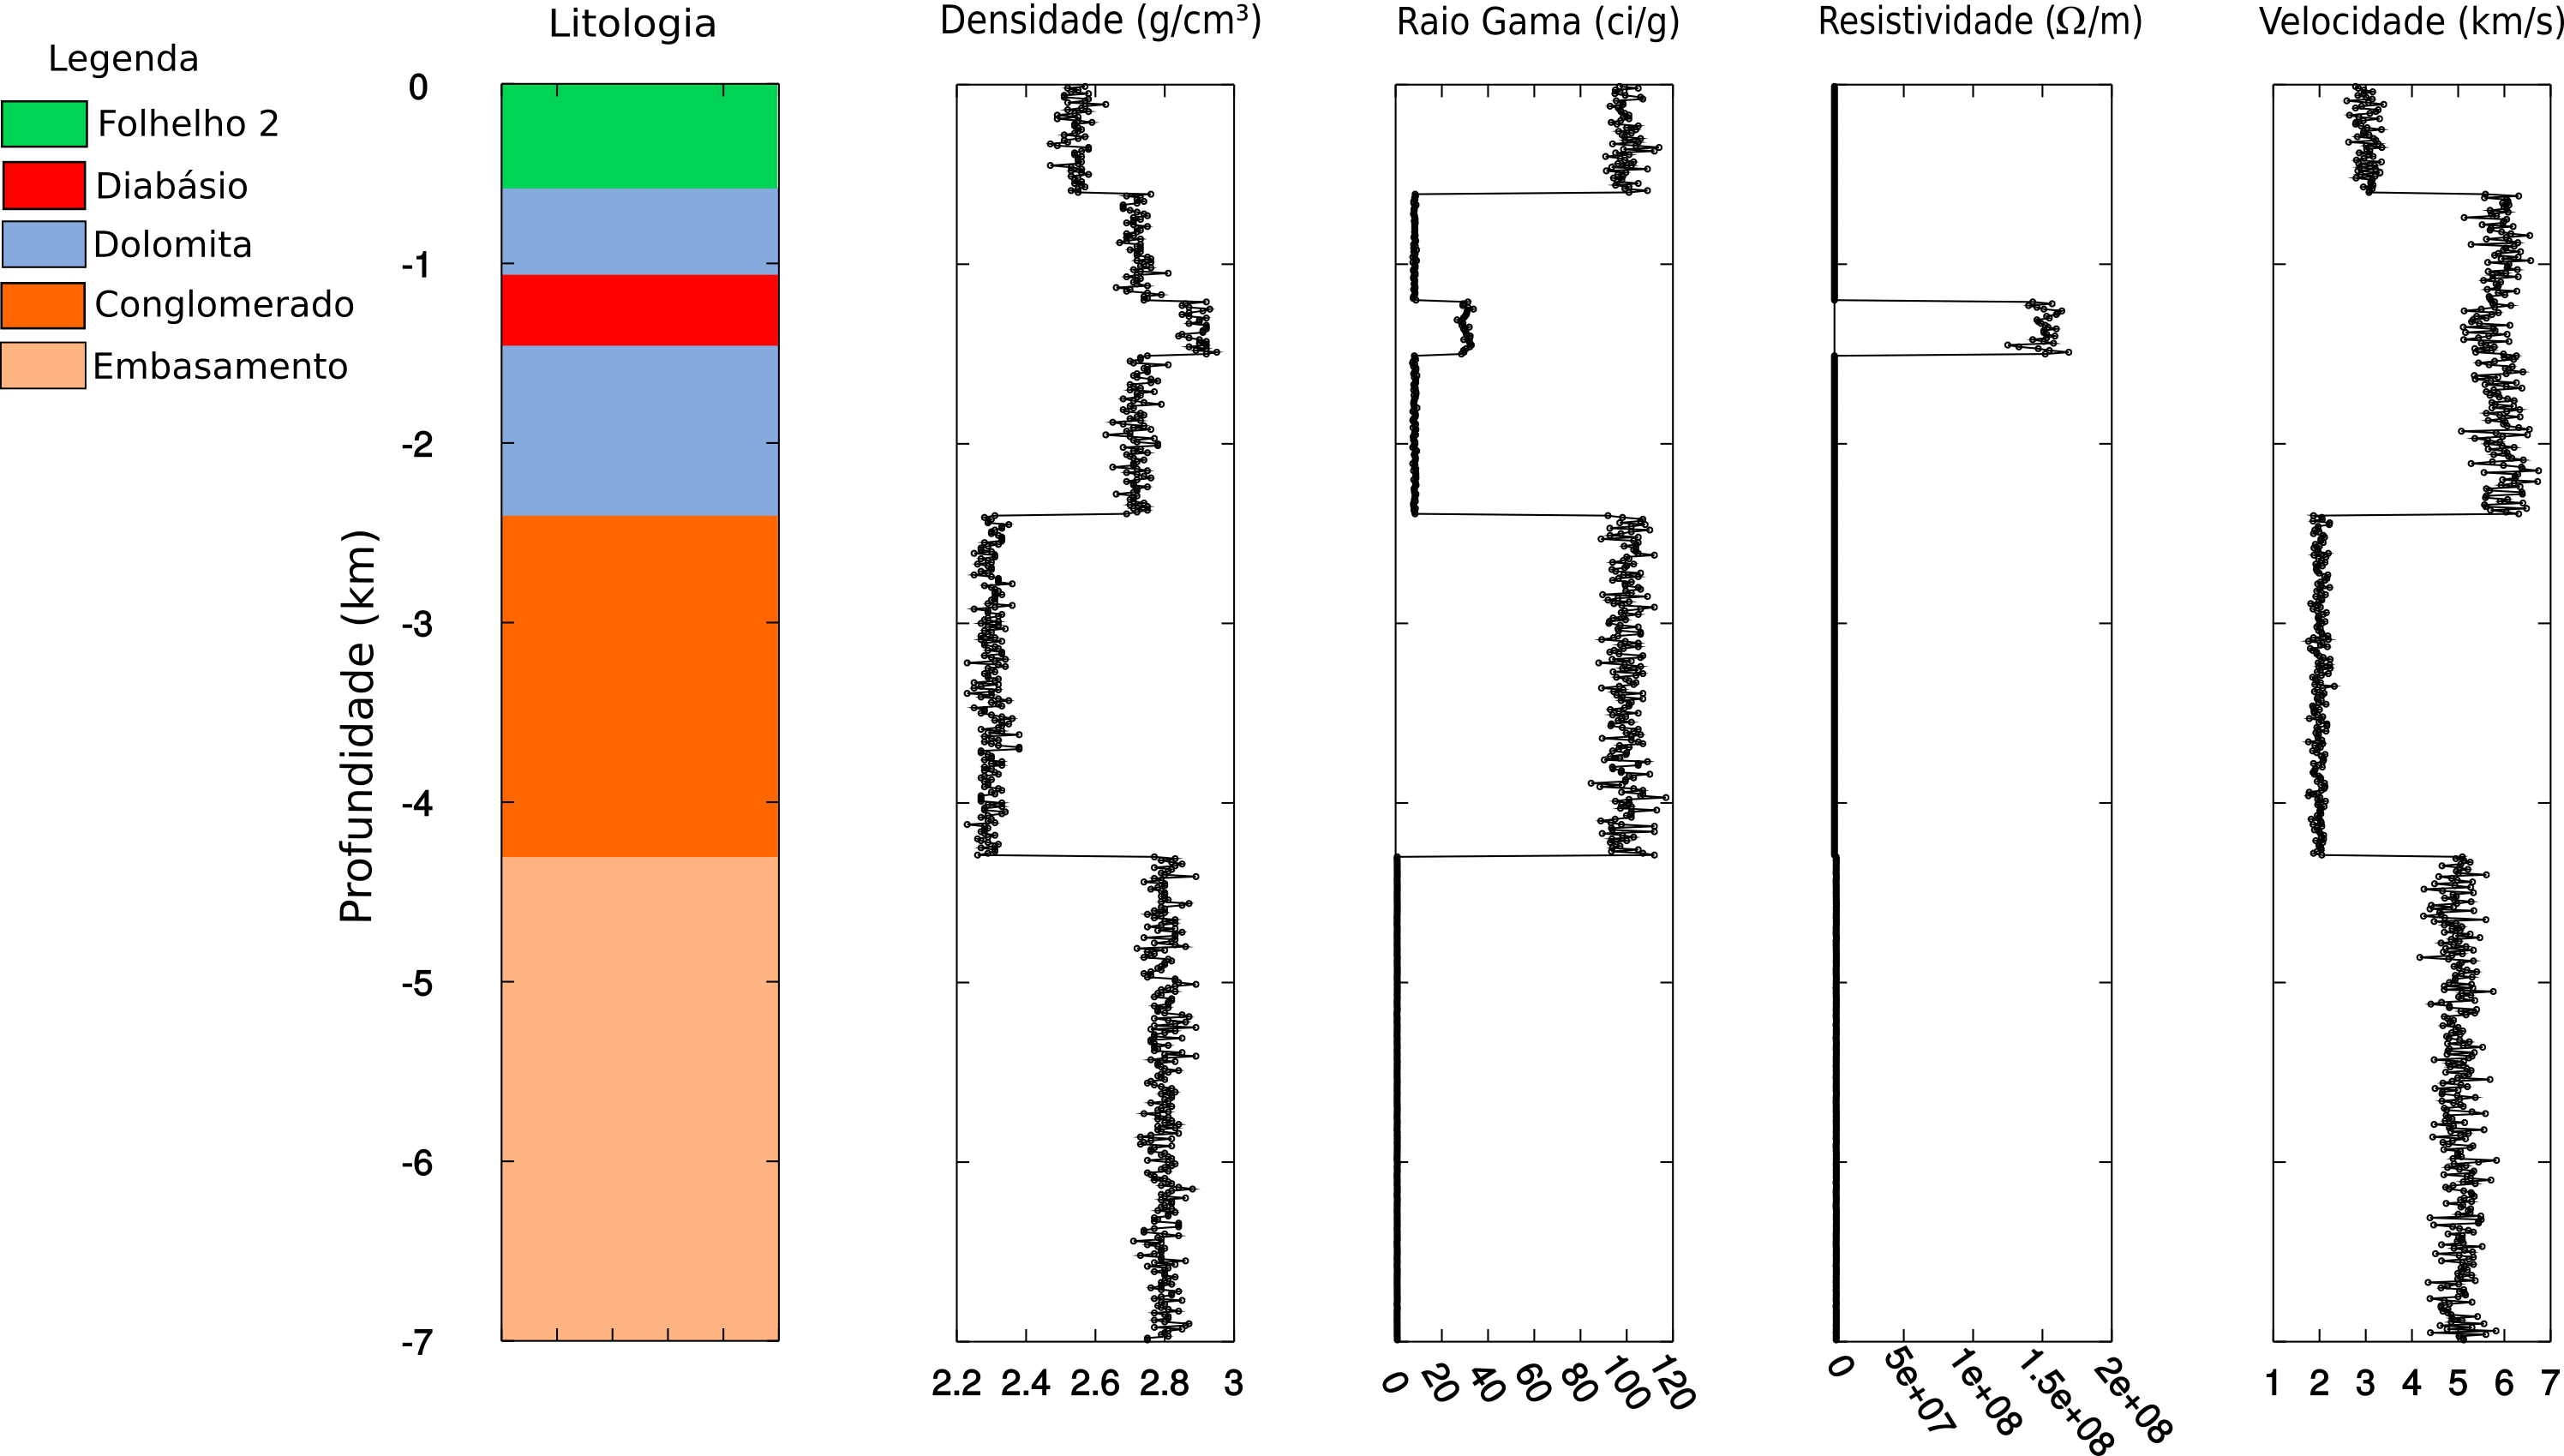
\includegraphics[scale=0.37]{Imagens/PocoC1.png}
\caption{Dado de perfilagem sintético, C1.}
\label{C1}
\end{figure}
\end{frame}

\begin{frame}
\frametitle{Modelo proposto}
\begin{figure}[H]
\centering
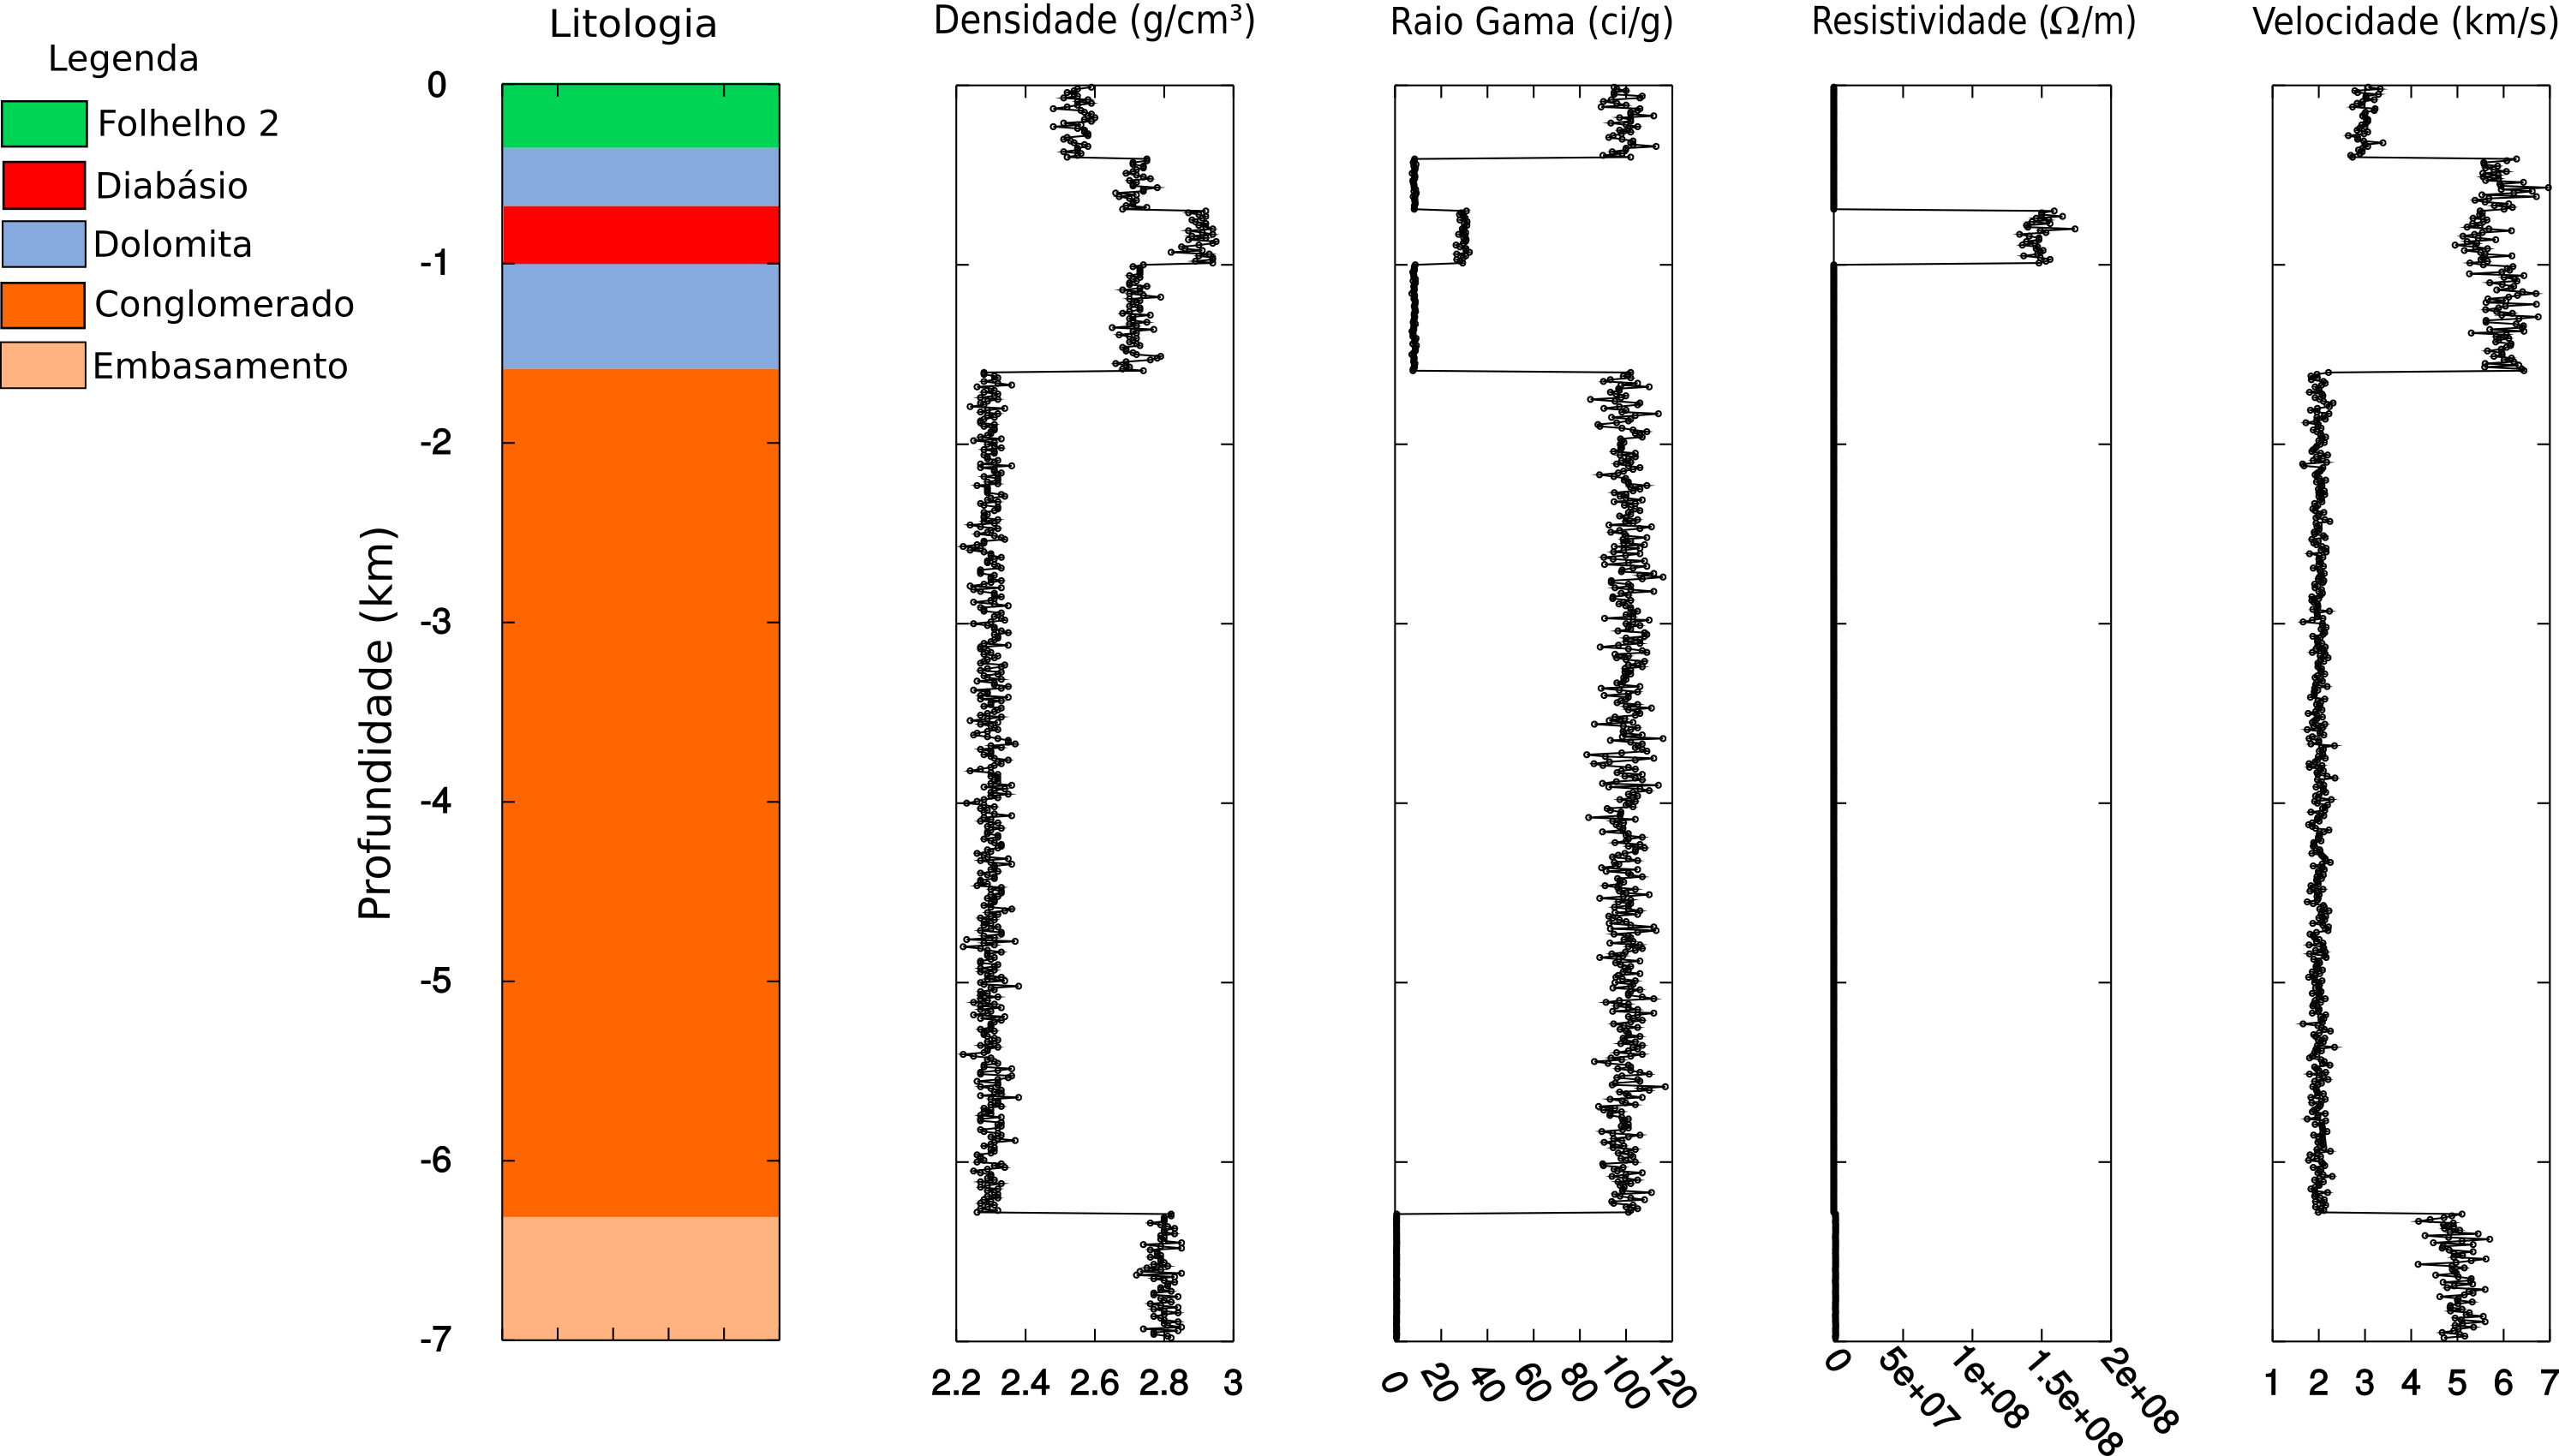
\includegraphics[scale=0.37]{Imagens/PocoC2.png}
\caption{Dado de perfilagem sintético, C2.}
\label{C2}
\end{figure}
\end{frame}

\begin{frame}
	\frametitle{Metodologia}
	\smartdiagram[priority descriptive diagram]{
		Geração do modelo de hipóteses,
		Poço T1 treinamento da rede e distâncias dos classificadores,
		Predição dos poços C1 e C2 com o SOM e os classificadores,
		Compara os resultados e aplica ao dado real.	}
\end{frame}


\subsubsection{Classificador euclideano}

\begin{frame}
	\frametitle{Classificador euclideano}
	\begin{tcolorbox}[colback=gray!5,colframe=blue!40!black,title=Definição]
		\begin{equation}
		Ed_{i} =  \Arrowvert \textbf{X}-\bar{\textbf{X}}_{i}  \Arrowvert_{2} \nonumber
		\label{eq4}
		\end{equation}  
	\end{tcolorbox}
	\pause
	\begin{itemize}
		\centering
		\item[$\textbf{X}$], vetor de atributos (entrada)
		\pause
		\item[$\bar{\textbf{X}}_{i}$], vetor média
	\end{itemize}
	
\end{frame}


\begin{frame}
	\frametitle{Classificador euclideano}
	\begin{figure}[H]
		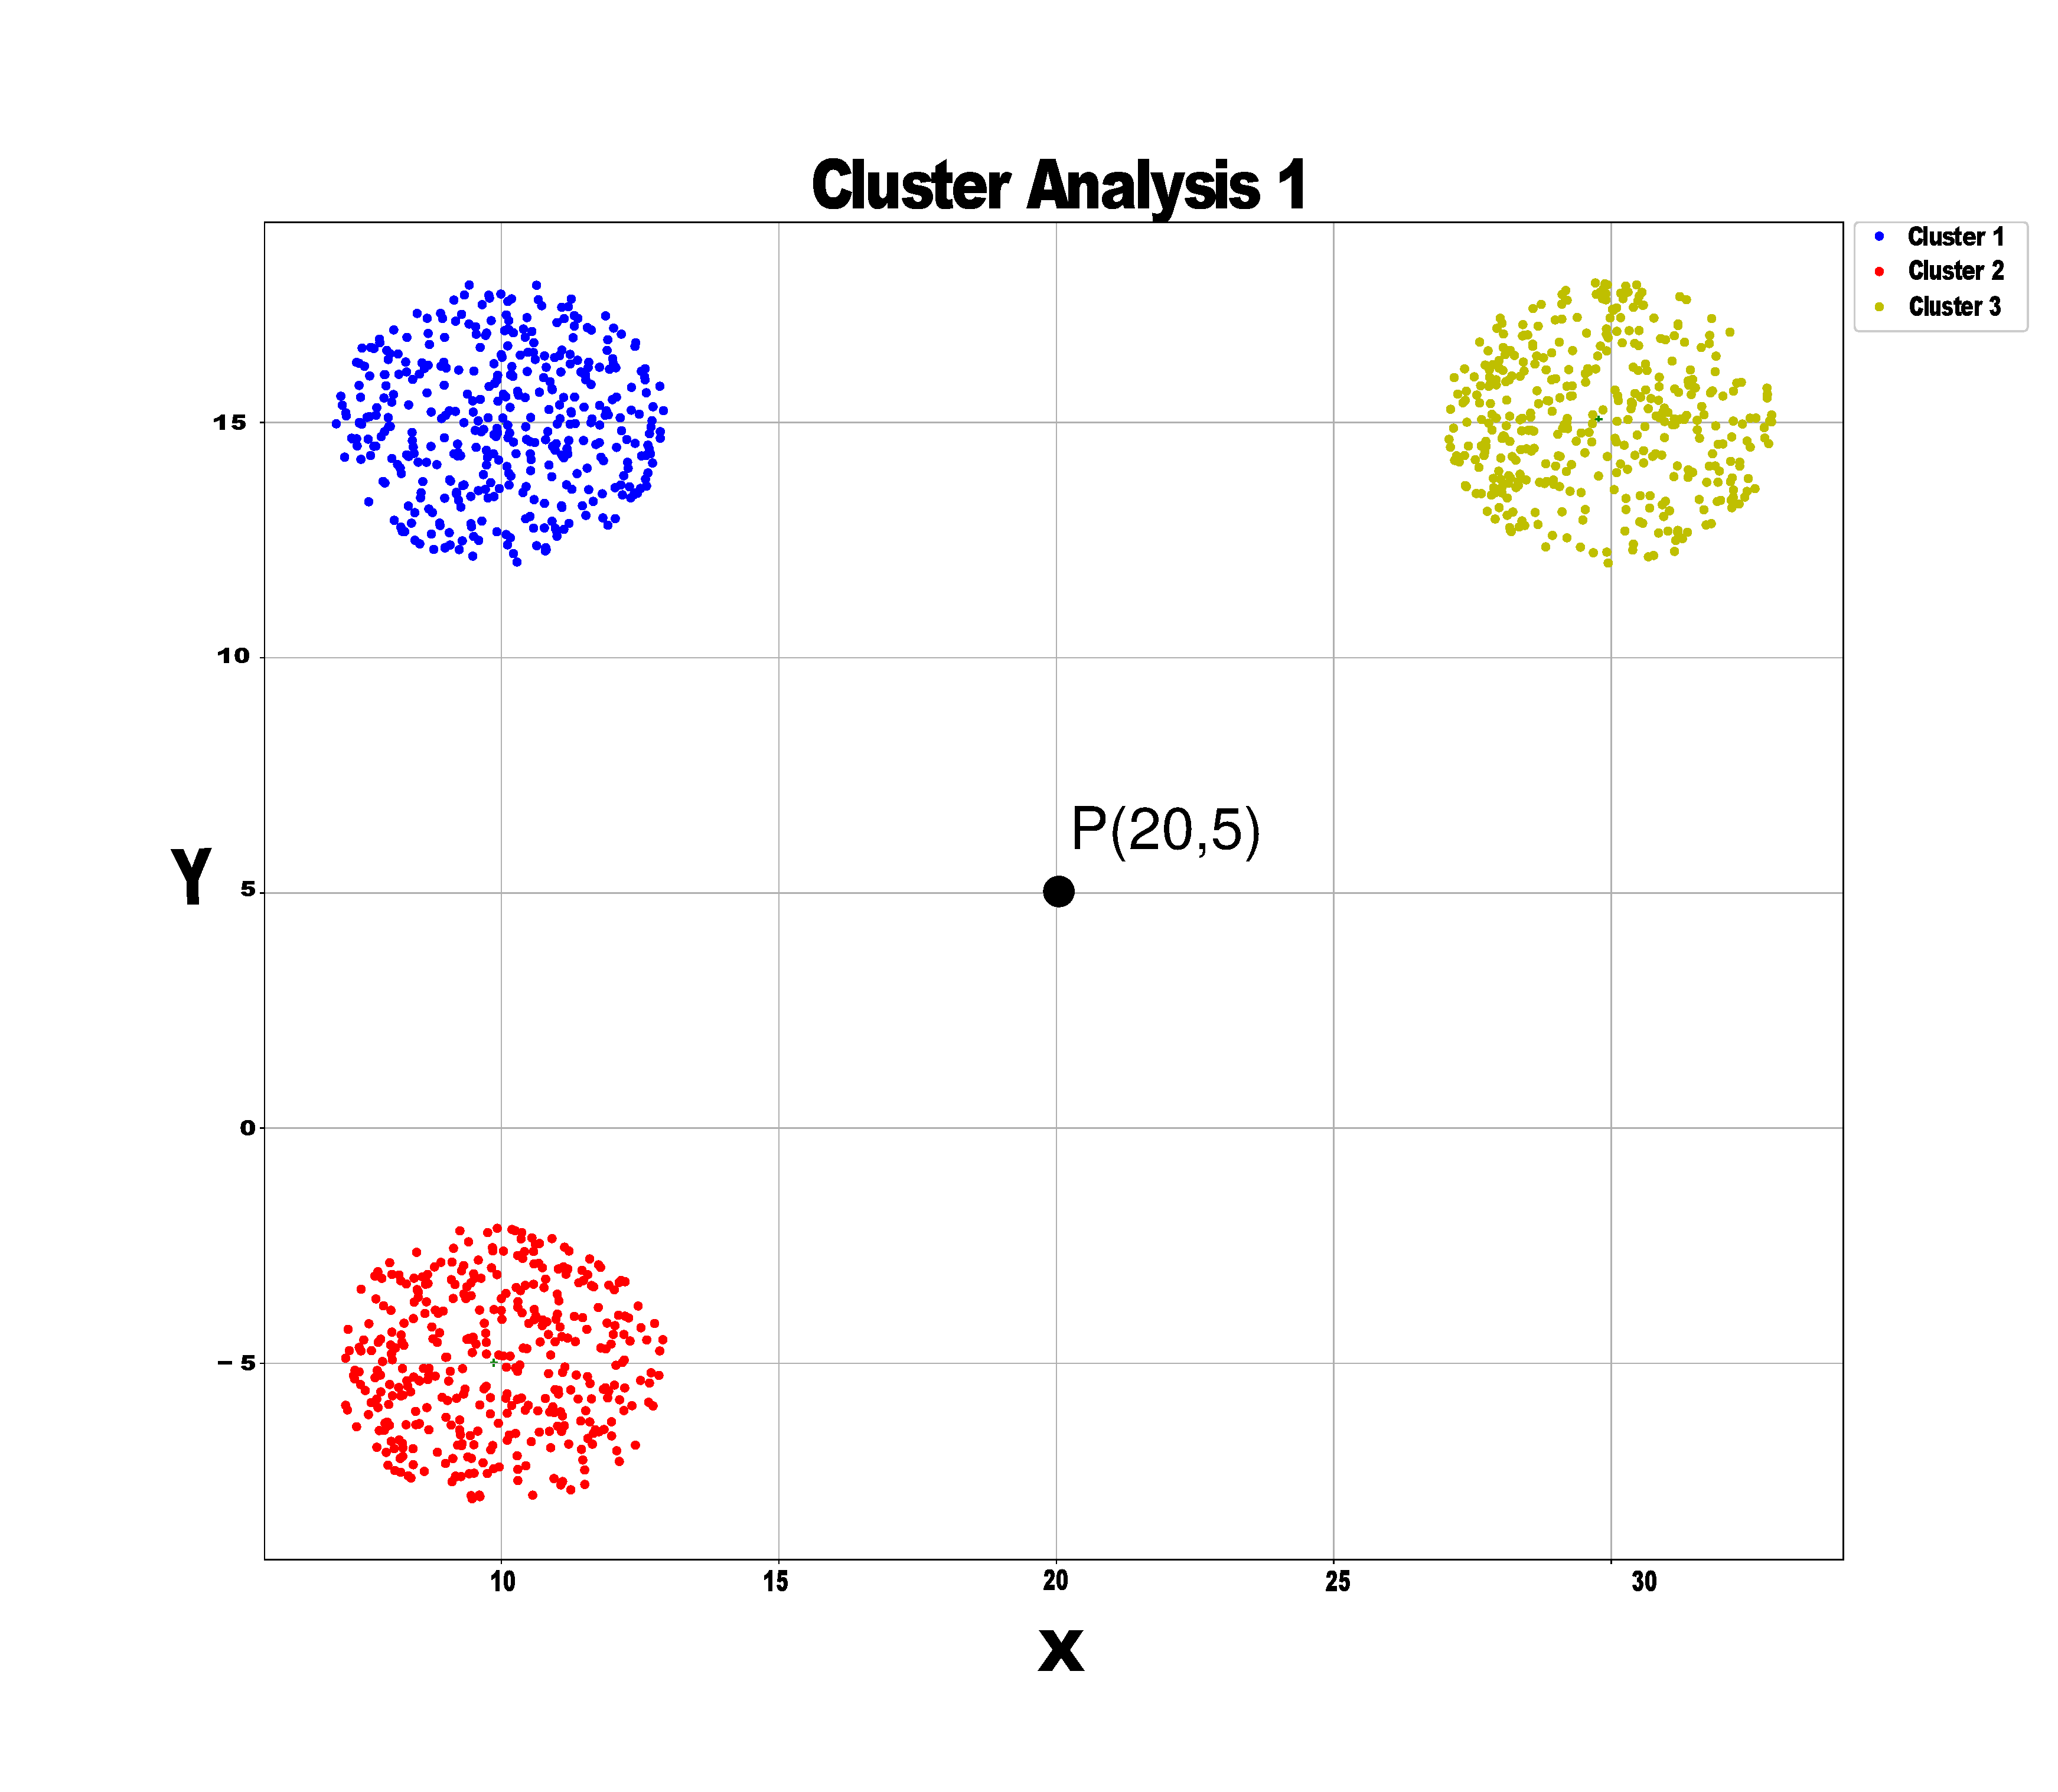
\includegraphics[scale=0.1]{Imagens/clusteranalise1.eps}
	\end{figure}
	
	\begin{columns}
		\column{1\textwidth}
		\footnotesize
		\justifying
		\begin{itemize}
			\footnotesize
			\item  Todos os centroides são equidistantes 
			\pause
			\item P$(20,5)$ pode ser um membro de todos os grupos do ponto de vista euclideano  
		\end{itemize}
	\end{columns}
	
\end{frame}

\begin{frame}
	\frametitle{Classificador euclideano}
	\begin{figure}[H]
		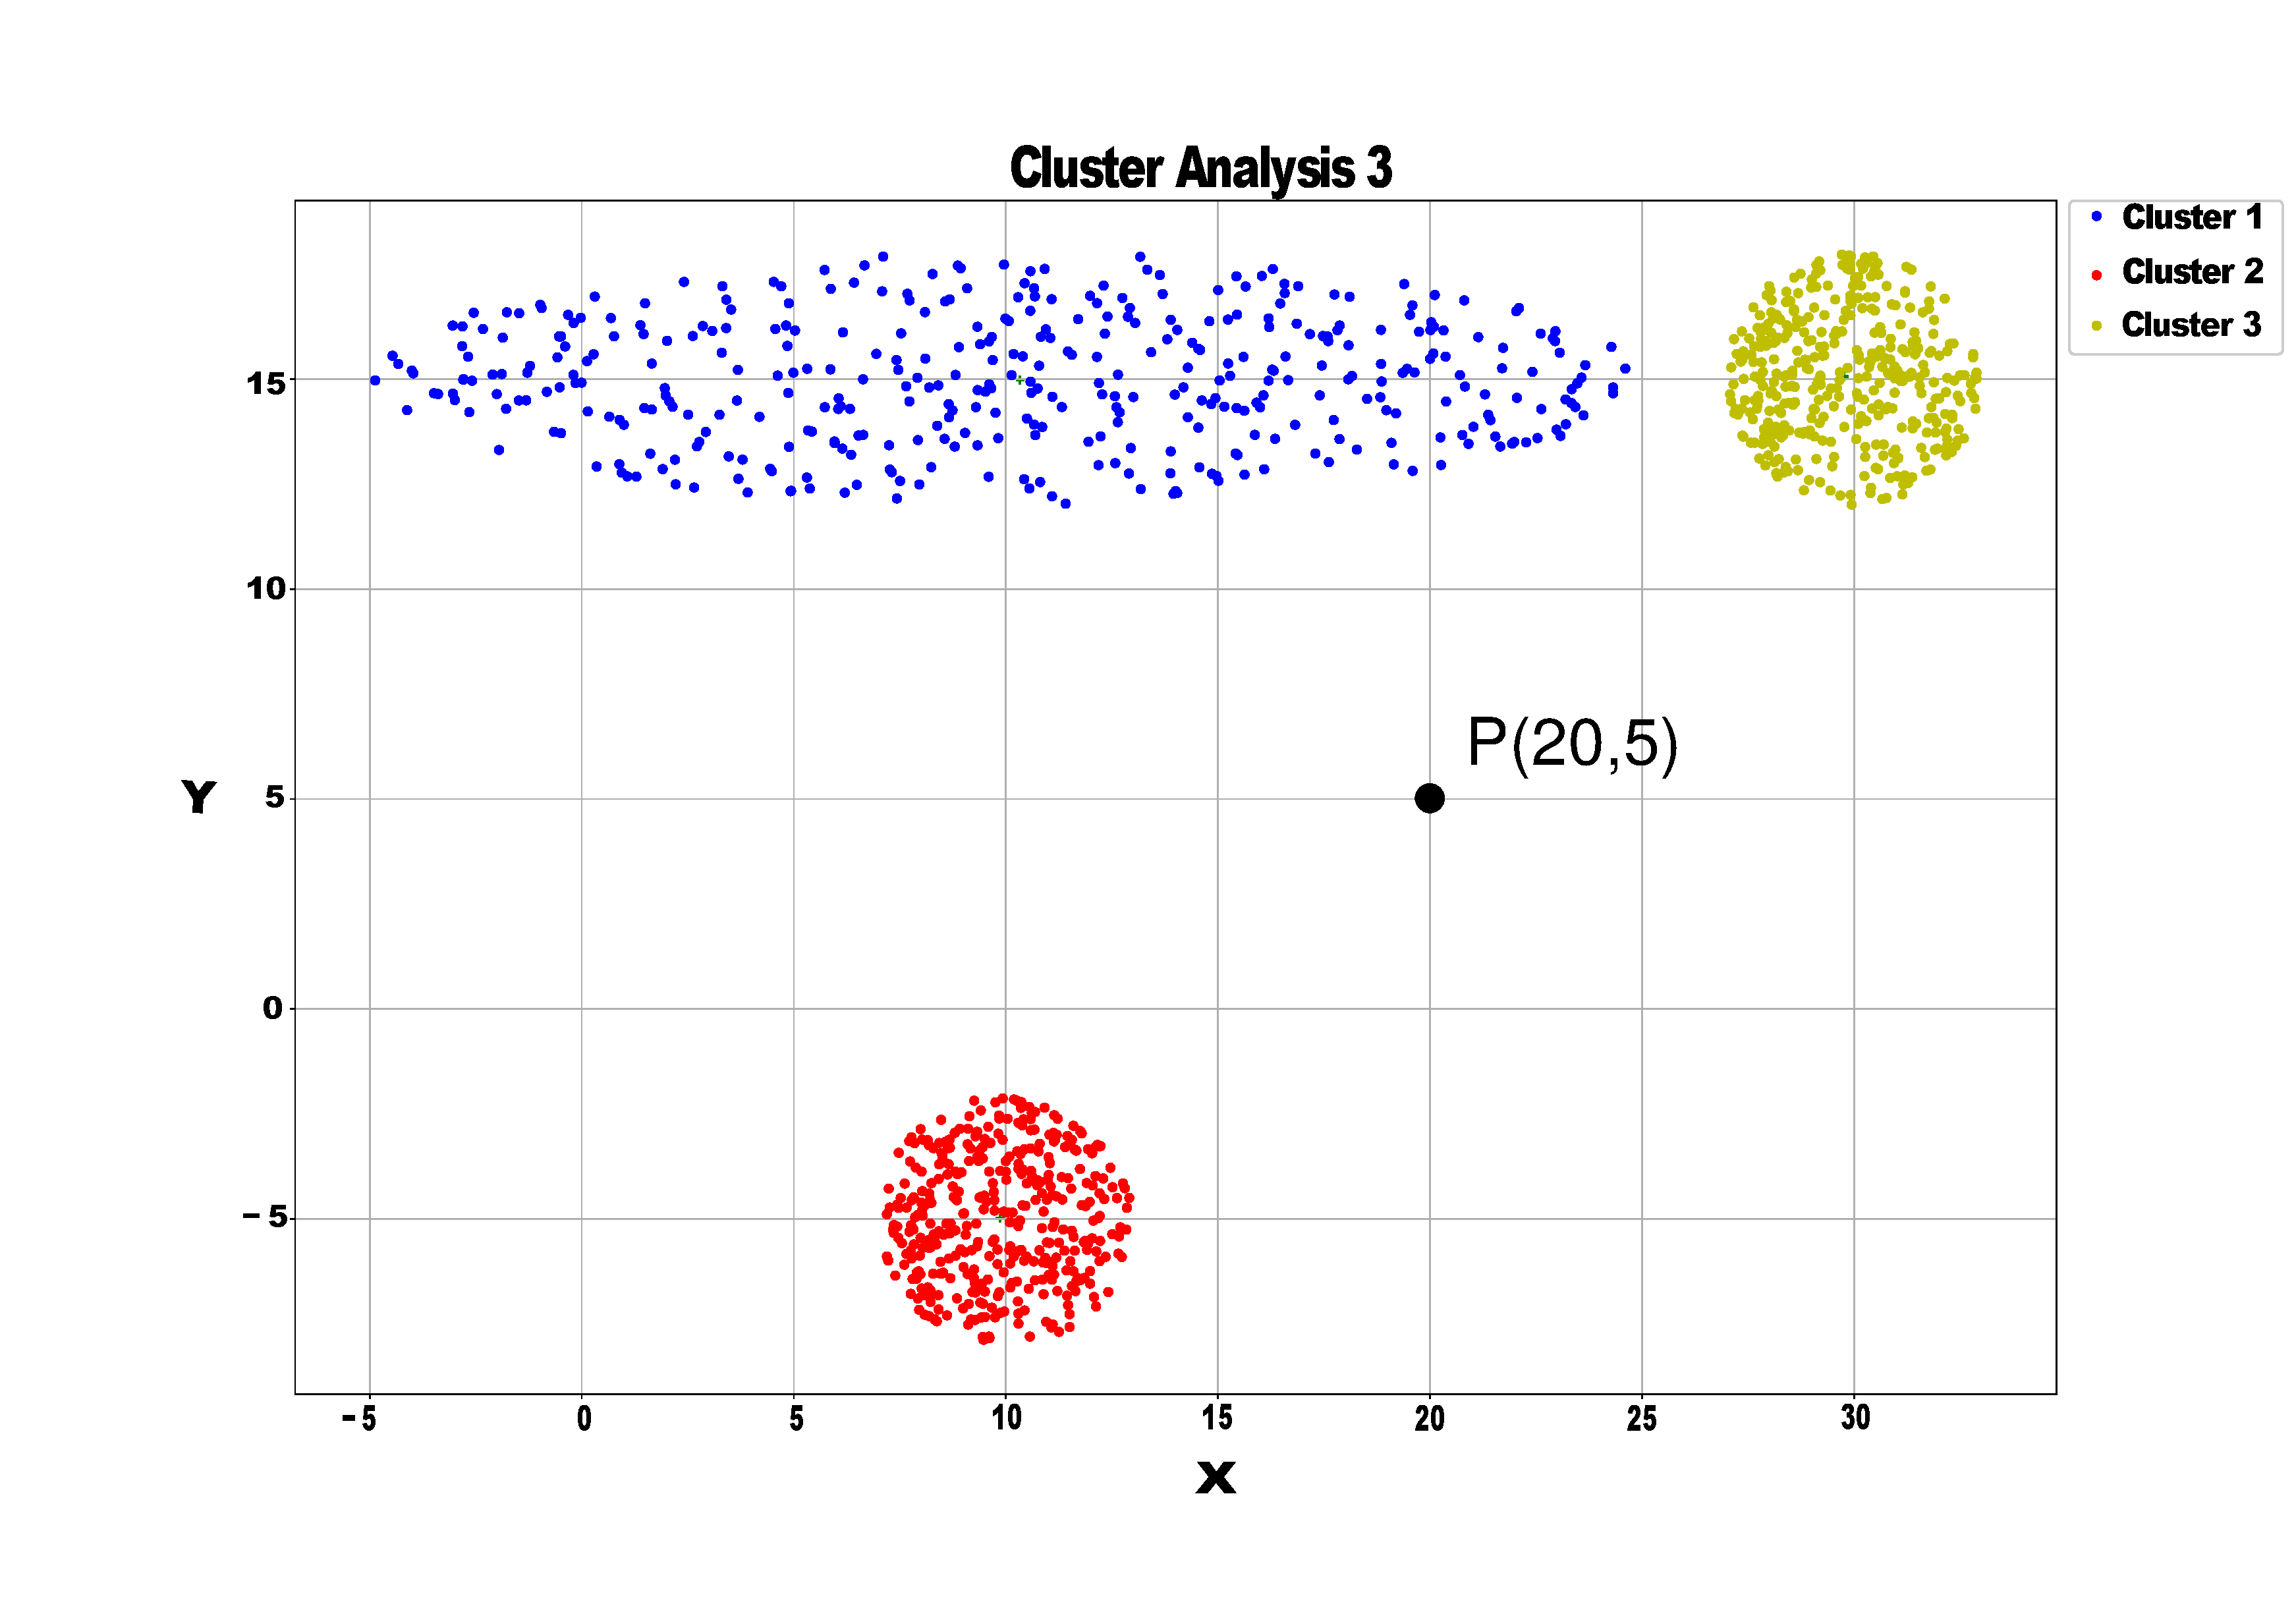
\includegraphics[scale=0.12]{Imagens/clusteranalise3.eps}
	\end{figure}
	
	\begin{columns}
		\column{1\textwidth}
		\footnotesize
		\justifying
		\begin{itemize}
			\item O agrupamento azul continua com o mesmo centroide
			\pause 
			\item A problemática jaz em definir qual agrupamento o ponto  P$(20,5)$ pertencerá 
			\pause
			\item Como resolve-se esta problemática?
		\end{itemize}
	\end{columns}
\end{frame}

\subsubsection{Classificador de Mahalanobis}

\begin{frame}
	\frametitle{Classificador de Mahalanobis}
	\begin{tcolorbox}[colback=gray!5,colframe=blue!40!black,title=Definição]
		\begin{equation}
		Md_{i}=\Arrowvert(\textbf{X}-\bar{\textbf{X}}_{i})^{T}\textbf{C}_{i}^{-1}(\textbf{X}-\bar{\textbf{X}}_{i})\Arrowvert_{2}\nonumber
		\label{eq5}
		\end{equation}
	\end{tcolorbox}
	\pause
	\begin{itemize}
		\centering
		\item[$\textbf{X}$], vetor de atributos (entrada)
		\pause
		\item[$\bar{\textbf{X}}_{i}$], vetor média
		\pause
		\item[$\textbf{C}_{i}$], matriz de covariância 
	\end{itemize}
\end{frame}


%\begin{frame}
%\frametitle{Mahalanobis Classifier}
%
%\begin{equation}
%\textbf{C}_{i}=\frac{1}{n_{i}-1}\sum_{X \in \omega_{i}}(\textbf{X}-\bar{\textbf{X}}_{i})(\textbf{X}-\bar{\textbf{X}}_{i})^{T}
%\label{eq6}
%\end{equation}
%\pause
%\begin{itemize}
%	\centering
%	\item[$n_{i}$], number of elements  
%	\pause
%	\item[$\omega_{i}$], space of attributes
%\end{itemize}
%\end{frame}

\begin{frame}
	\frametitle{Classificador Euclideano}
	\begin{figure}[H]
		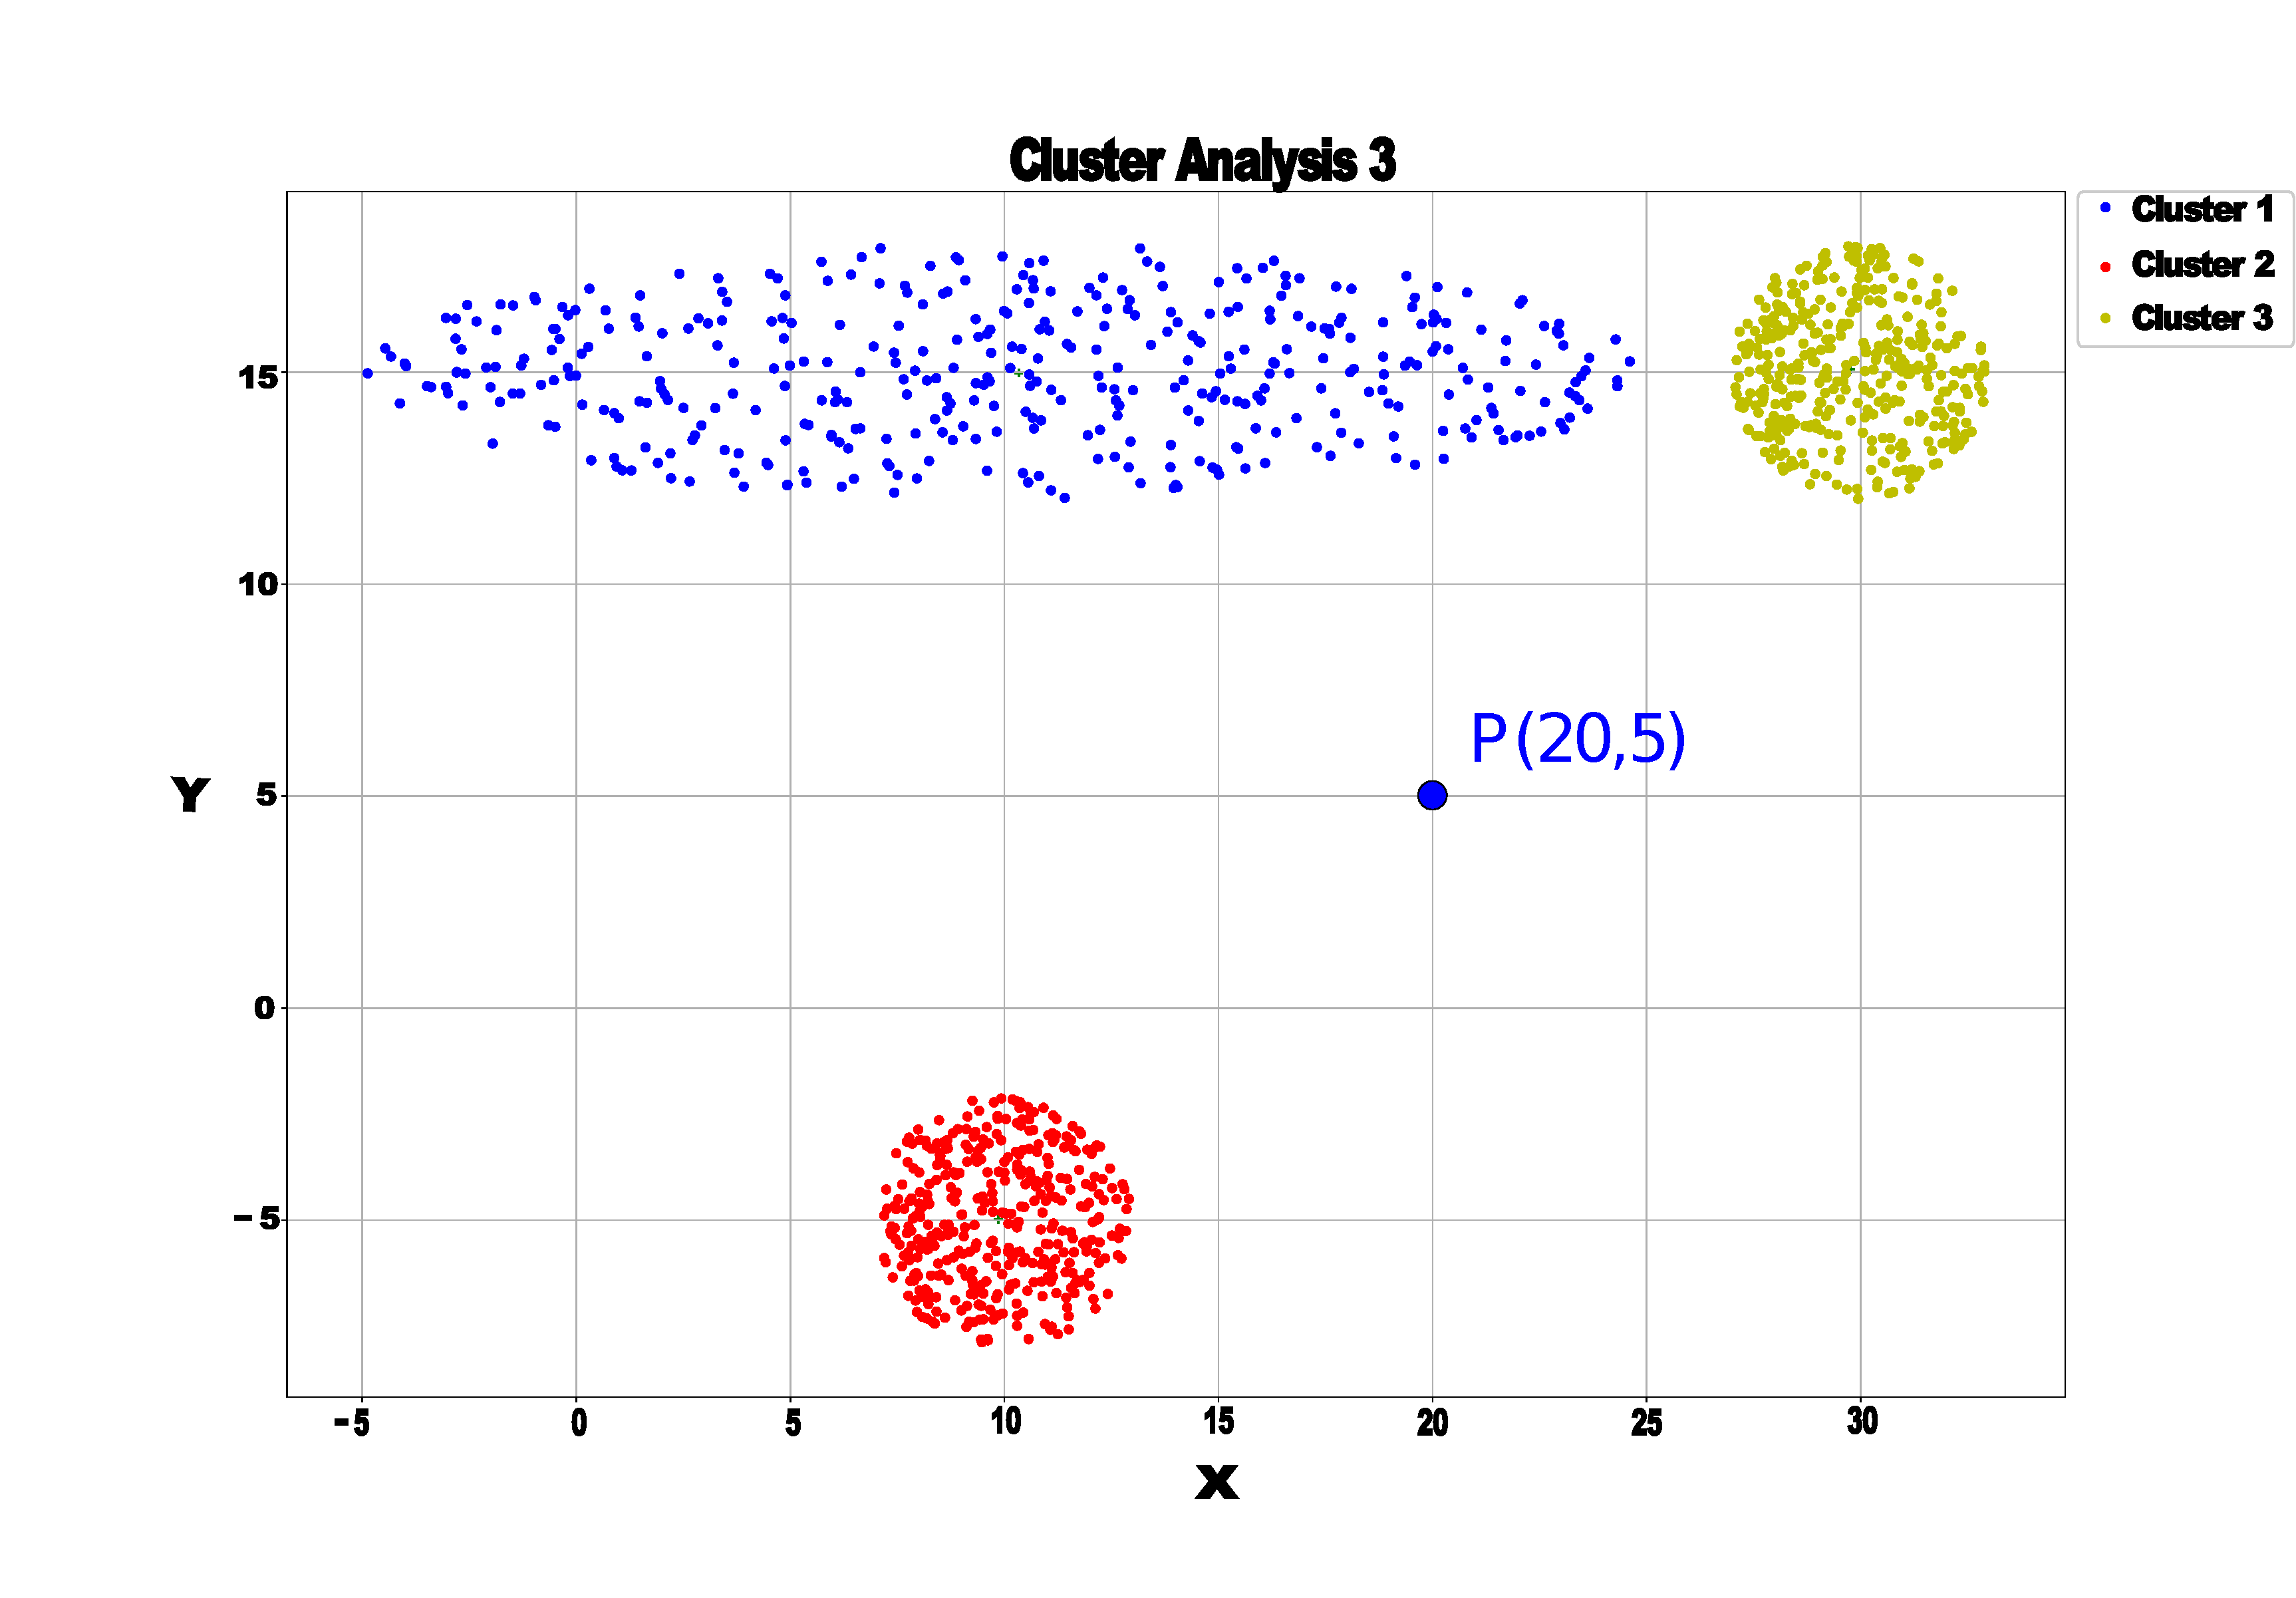
\includegraphics[scale=0.14]{Imagens/clusteranalise3blue.pdf}
	\end{figure}
	
	\begin{columns}
		\column{1\textwidth}
		\footnotesize
		\justifying
		\begin{itemize}
			\item Agora, P$(20,5)$ pertence ao  \textcolor{blue}{agrupamento $1$}.
		\end{itemize}
	\end{columns}
\end{frame}

\begin{frame}
	\begin{huge}
		\centering
		Voltando ao problema ...
	\end{huge}
\end{frame}

\subsubsection{Agrupamento e o espaço de atributos}

\begin{frame}
	\frametitle{Analise de agrupamento: poço T1}
	\begin{columns}
		\column{0.5\textwidth}
		\footnotesize
		\justifying
		\begin{figure}
			%\centering
			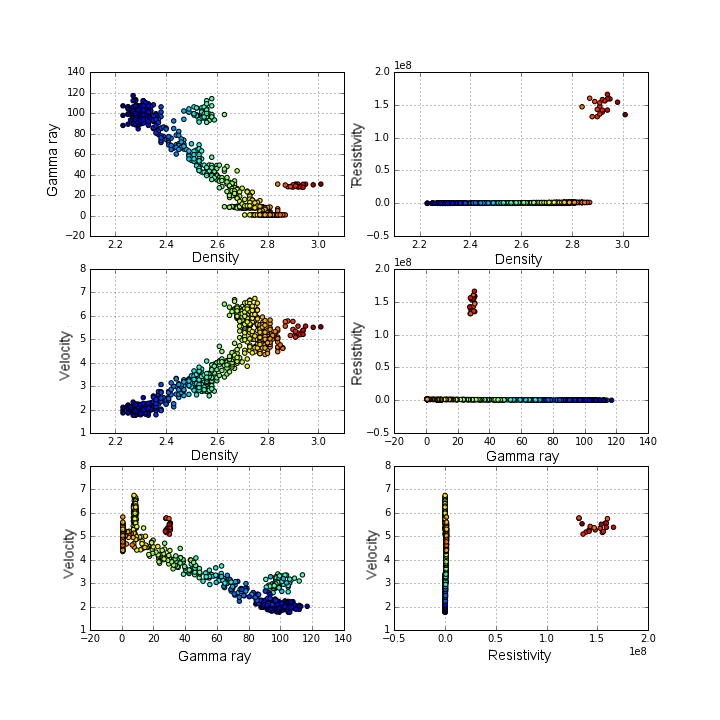
\includegraphics[scale=0.268]{Imagens/cluterpocoT1.png}
		\end{figure}
		
		\column{0.3\textwidth}
		\begin{itemize}
			\footnotesize
			\item Análise de dispersão em pares de propriedades ($6$ gráficos);
			\pause
			\item as cores representam, a variação das propriedades físicas;
			\pause
			\item alguns agrupamentos elongados;
			\pause
			\item outros misturados.
		\end{itemize}
		
	\end{columns}
\end{frame}


\begin{frame}
	\frametitle{Análise de agrupamento: poço C1}
	
	\begin{columns}
		\column{0.5\textwidth}
		\footnotesize
		\justifying
		\begin{figure}
			%\centering
			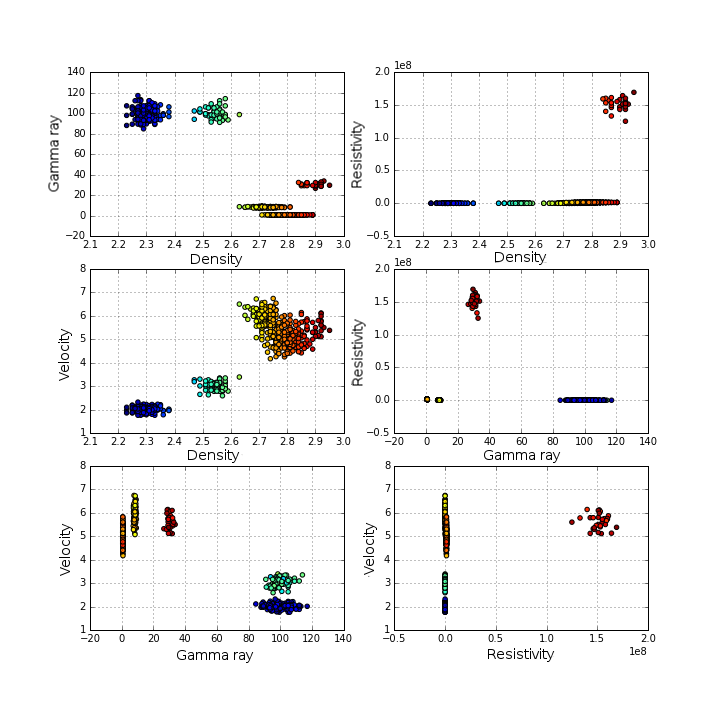
\includegraphics[scale=0.268]{Imagens/cluterpocoC1.png}
		\end{figure}
		
		\column{0.3\textwidth}
		\begin{itemize}
			\footnotesize
			\item Agrupamentos bem definidos;
			\pause
			\item Difere do poço de treinamento
		\end{itemize}
		
	\end{columns}
\end{frame}

\begin{frame}
	\frametitle{Análise de agrupamento: poço C2}
	
	\begin{columns}
		\column{0.5\textwidth}
		\footnotesize
		\justifying
		\begin{figure}
			%\centering
			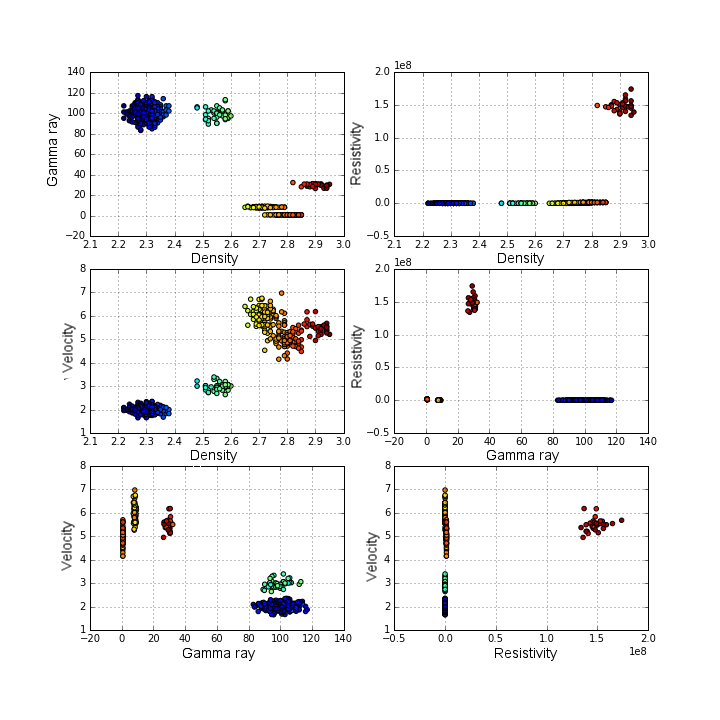
\includegraphics[scale=0.268]{Imagens/cluterpocoC2.png}
		\end{figure}
		
		\column{0.3\textwidth}
		\begin{itemize}
			\footnotesize
			\item Similar ao poço C1
		\end{itemize}
		
	\end{columns}
\end{frame}

\subsubsection{Kohonen - SOM}


\begin{frame}
	\frametitle{Treinamento não-supervisionado}
	\begin{itemize}
		\item  Insere-se na rede os atributos de entrada;
		\pause
		\item Os valores de saída são definidos pela própria rede;
		\pause
		\item Indicado para os casos aonde se tem agrupamento de dados;
		\pause
		\item Inspira-se no funcionamento do córtex cerebral \citep{Schott1993}.
	\end{itemize}
	
	\begin{figure}[H]
		\centering
		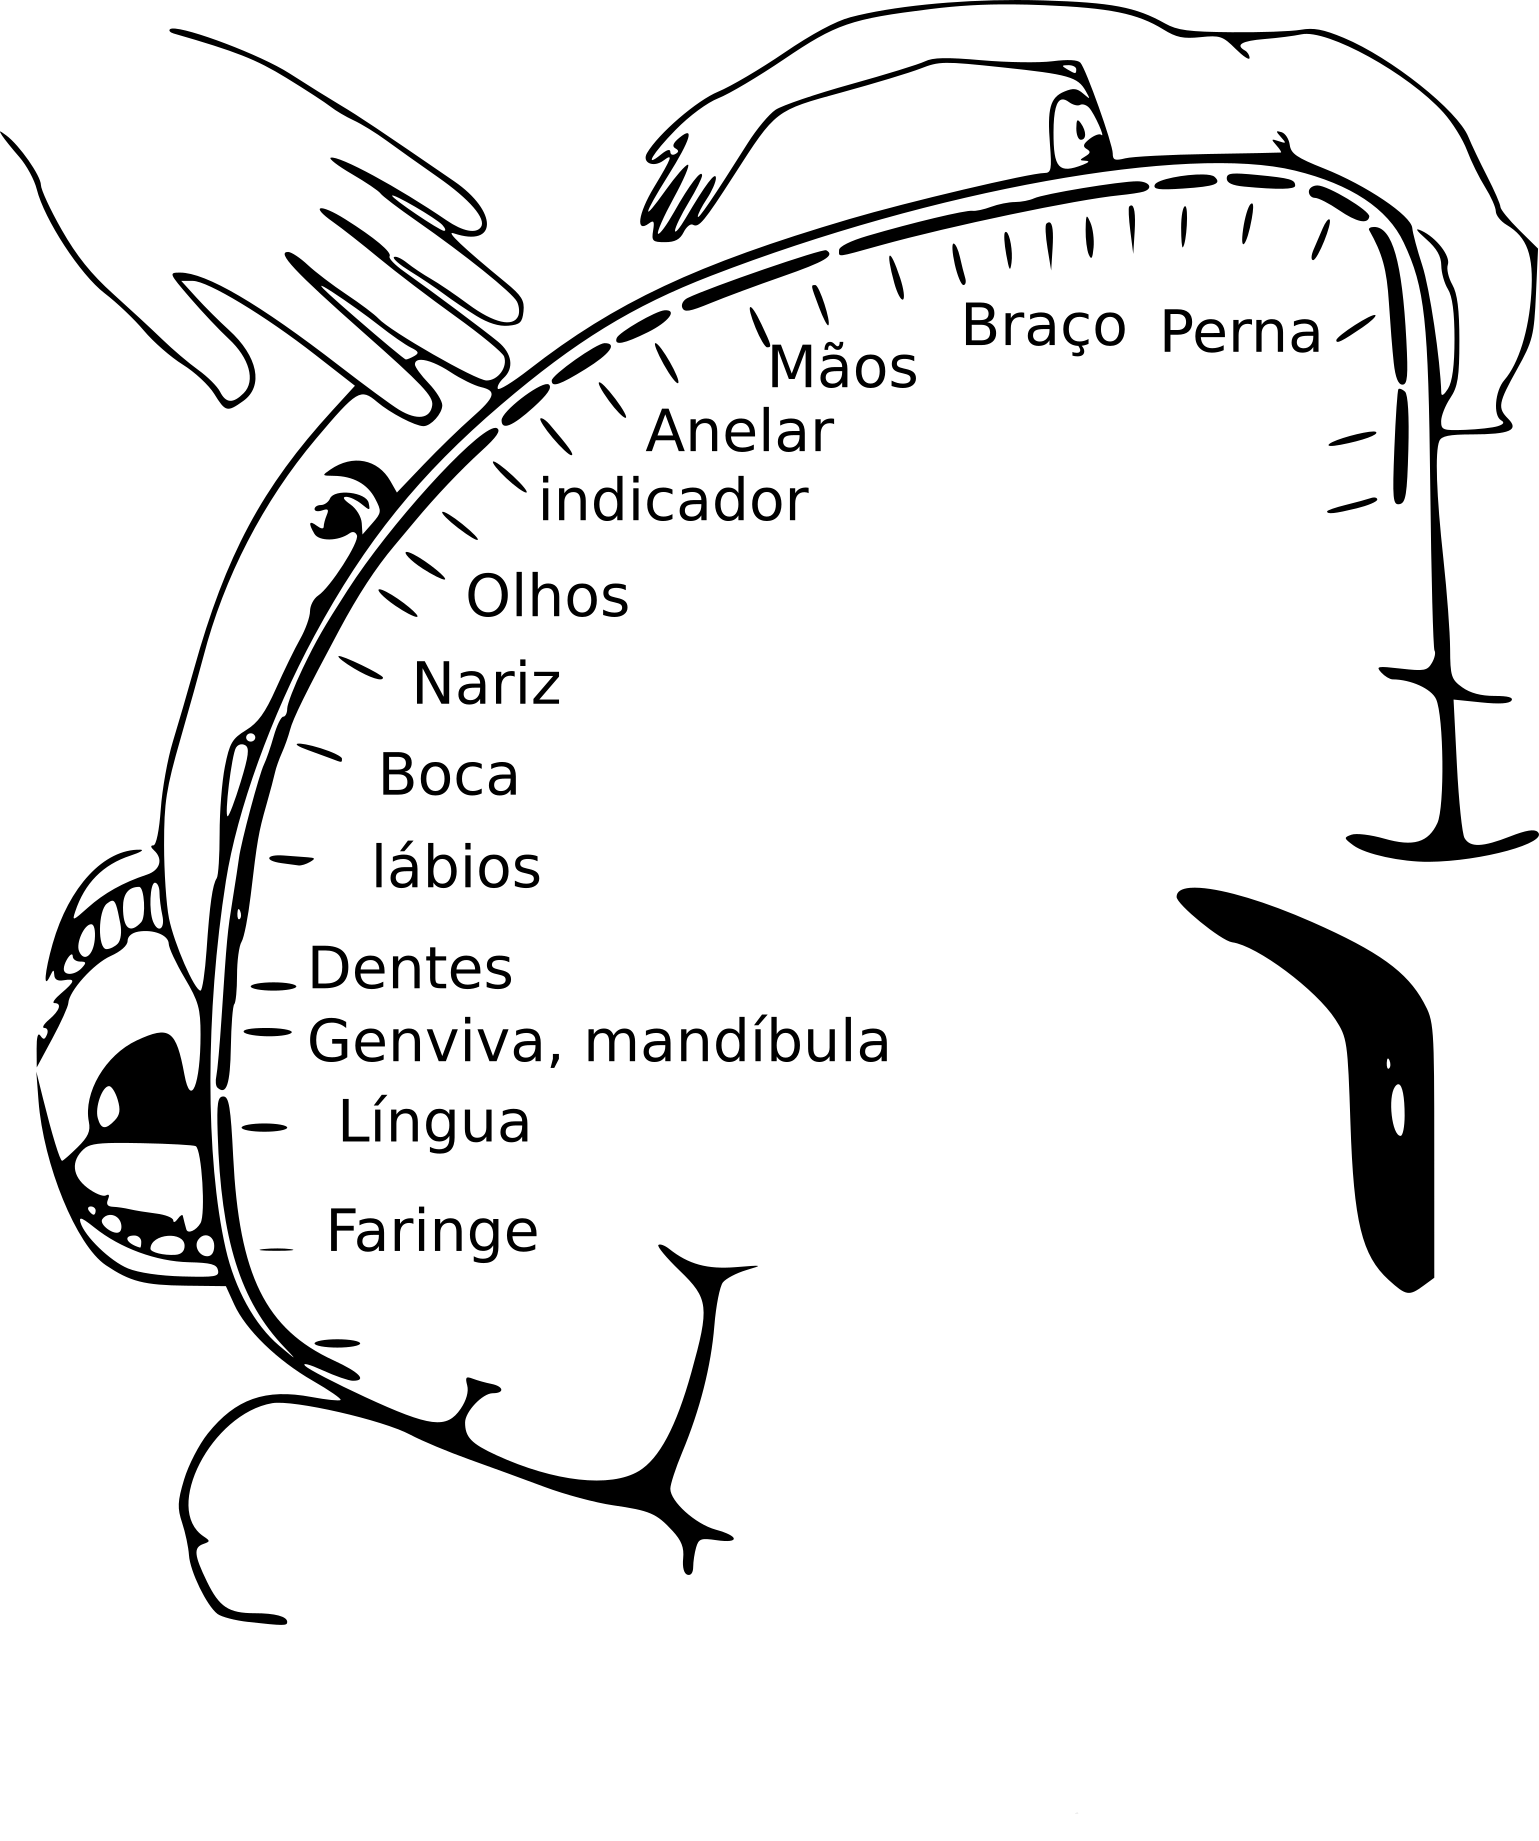
\includegraphics[scale=0.3]{Imagens/penfield.png}
		\caption{Homúnculo de Penfield }
		\label{penfield}
	\end{figure}
	
\end{frame}

\begin{frame}
	\frametitle{Kohonen - SOM}
	\framesubtitle{Organização}
	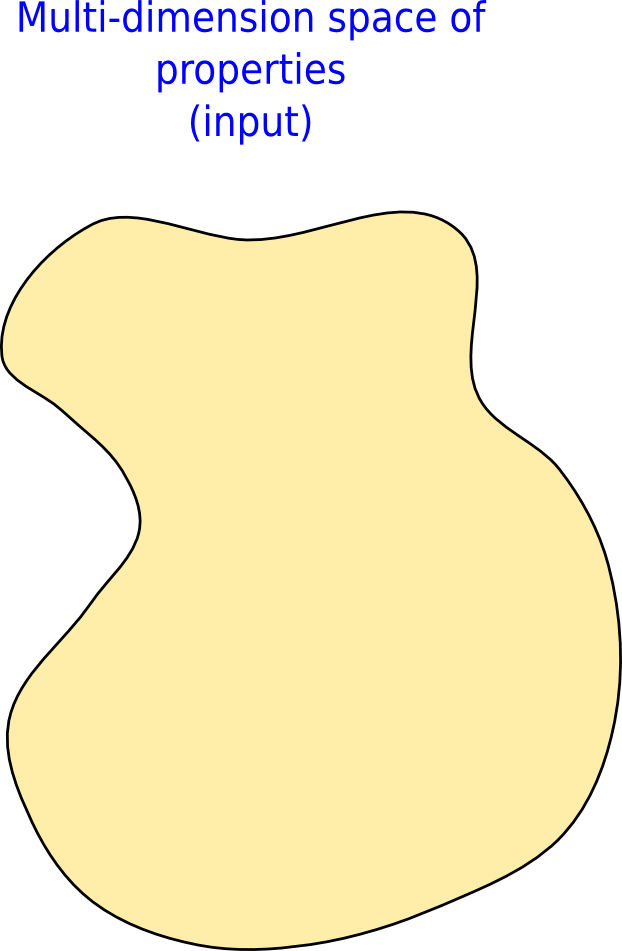
\includegraphics[scale=0.5]{Imagens/Introkoho1.png} 
\end{frame}


\begin{frame}
	\frametitle{Kohonen - SOM}
	\framesubtitle{Organização}
	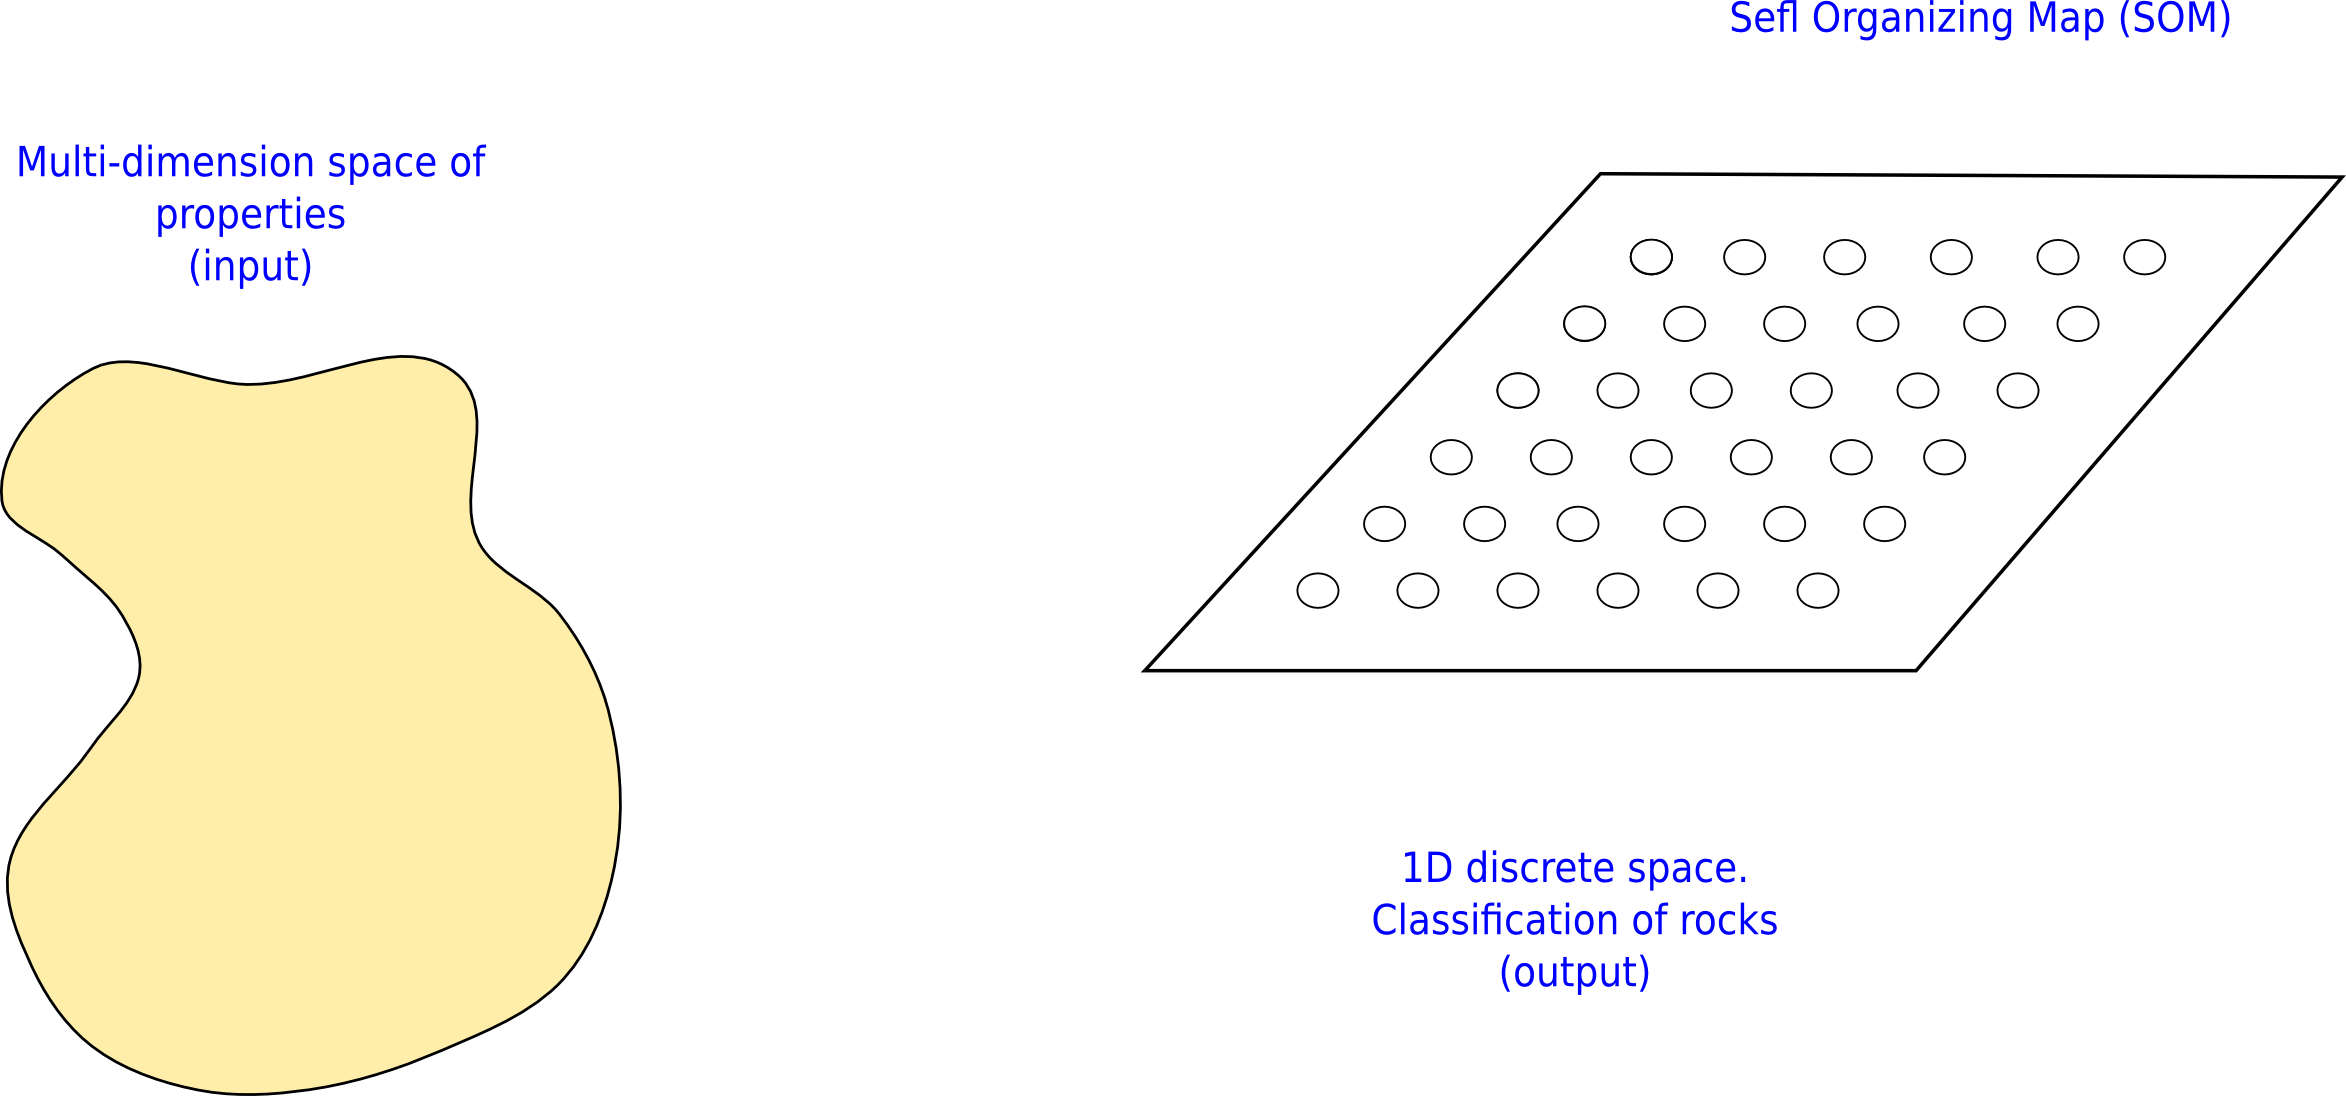
\includegraphics[scale=0.5]{Imagens/Introkoho2.png} 
\end{frame}


\begin{frame}
	\frametitle{Kohonen - SOM}
	\framesubtitle{Adaptação sináptica (Processo de treinamento)}
	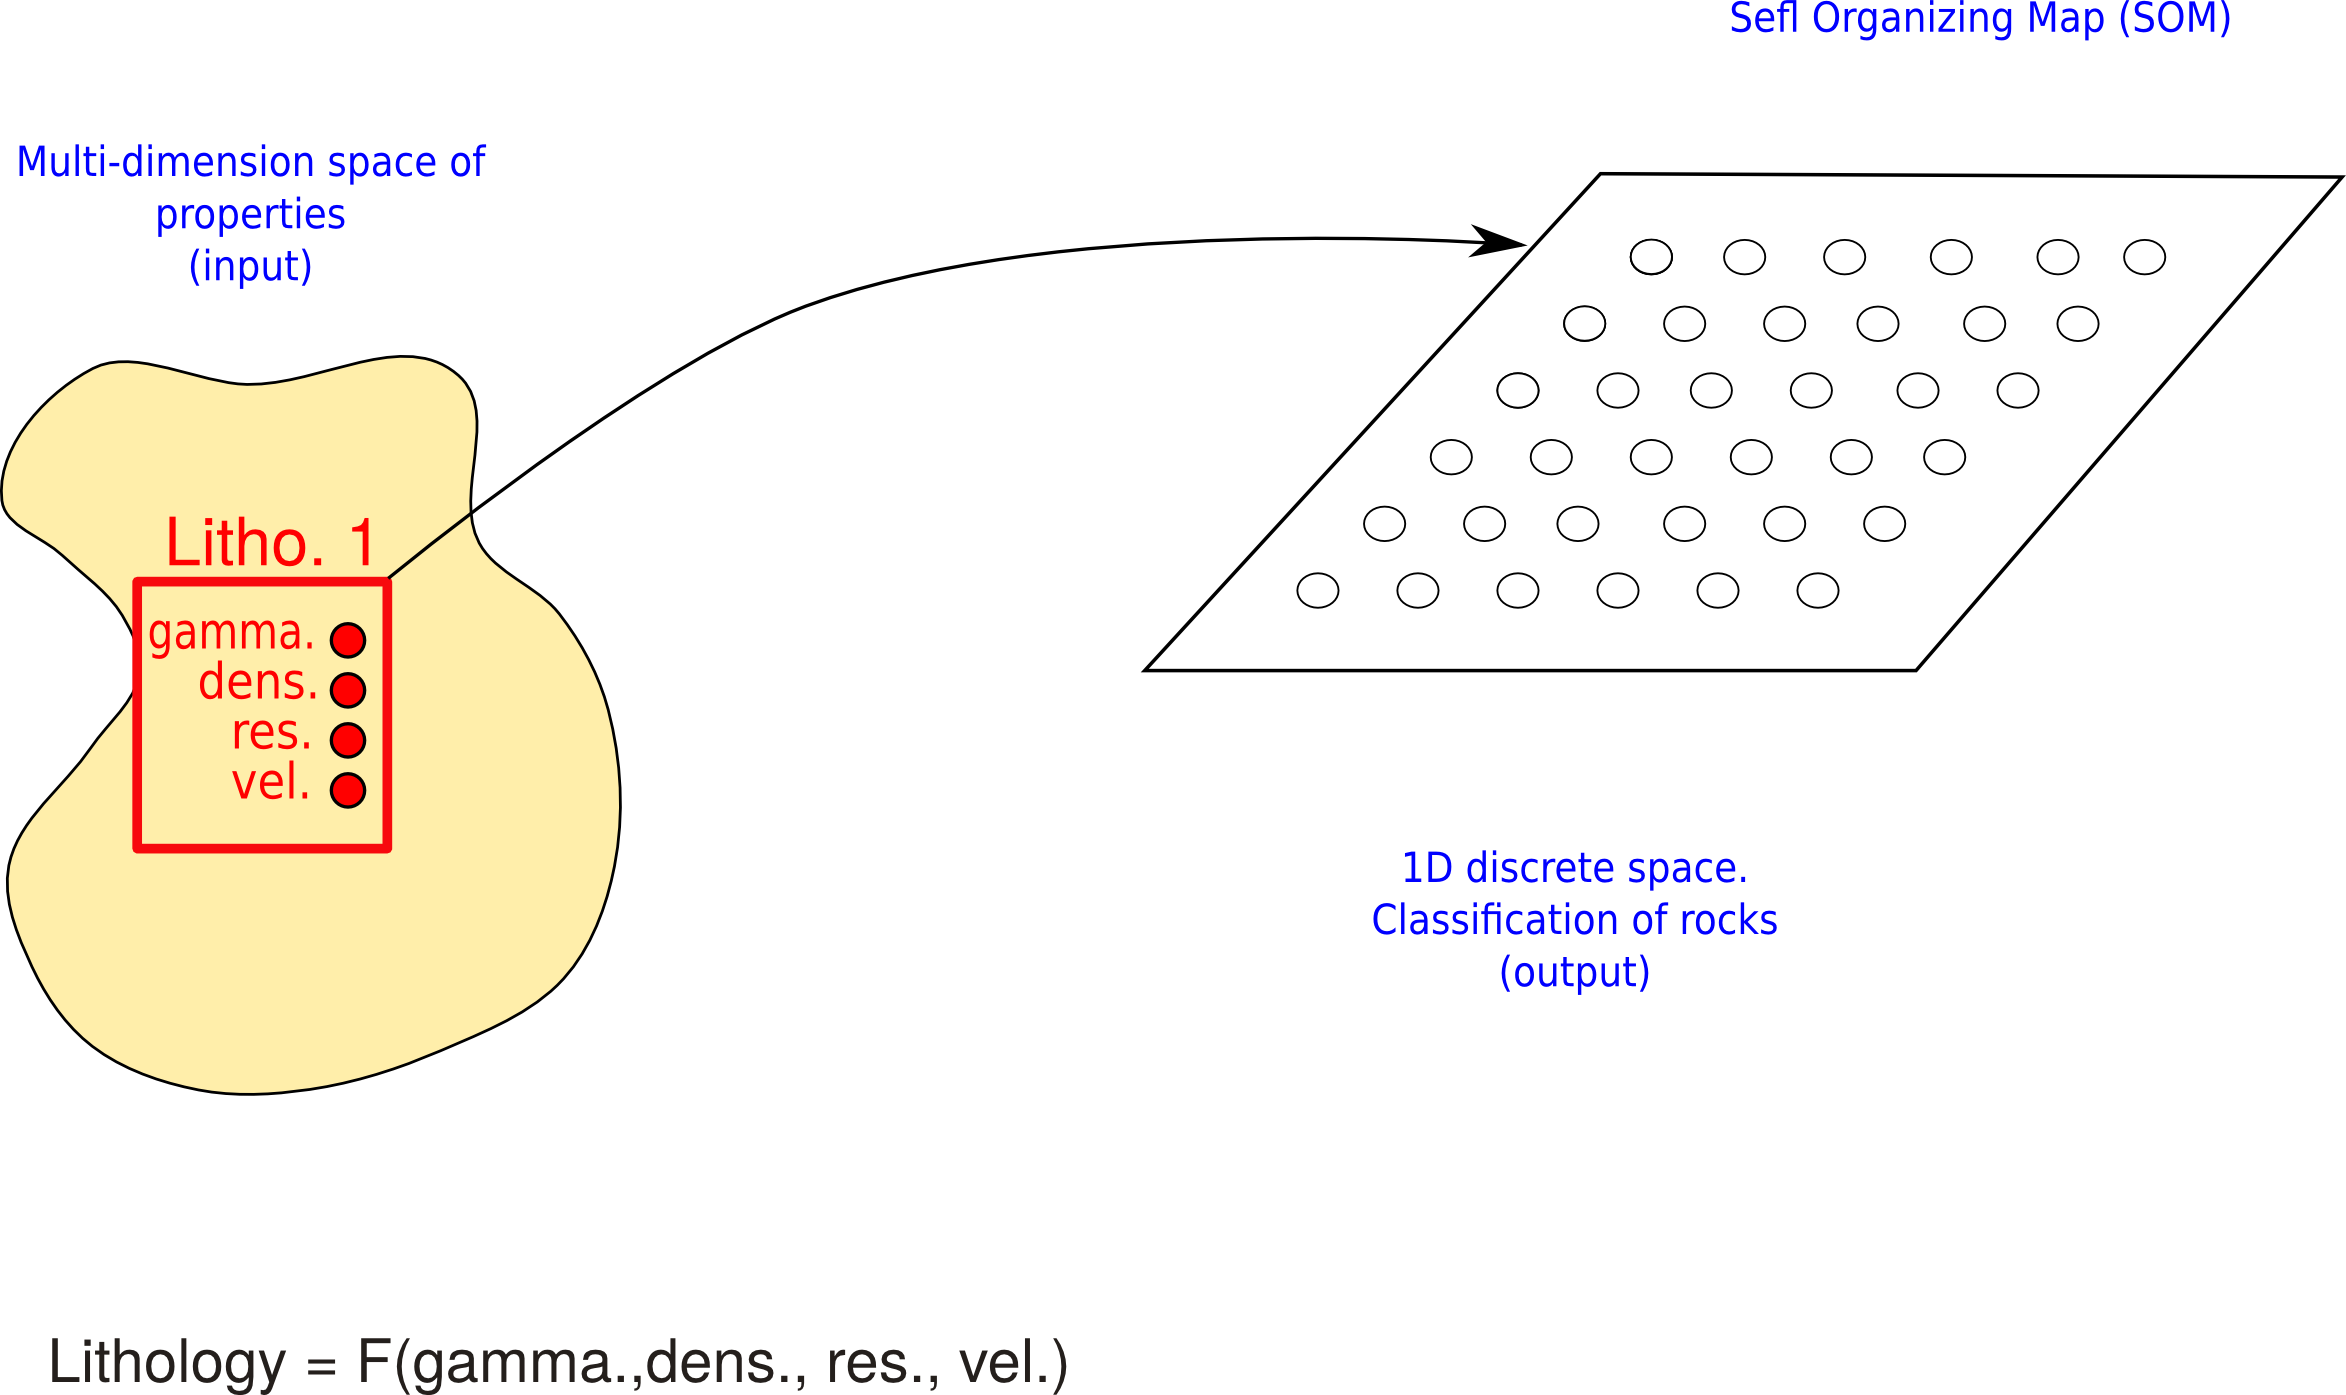
\includegraphics[scale=0.5]{Imagens/Introkoho3.png} 
\end{frame}


\begin{frame}
	\frametitle{Kohonen - SOM}
	\framesubtitle{Classificação}
	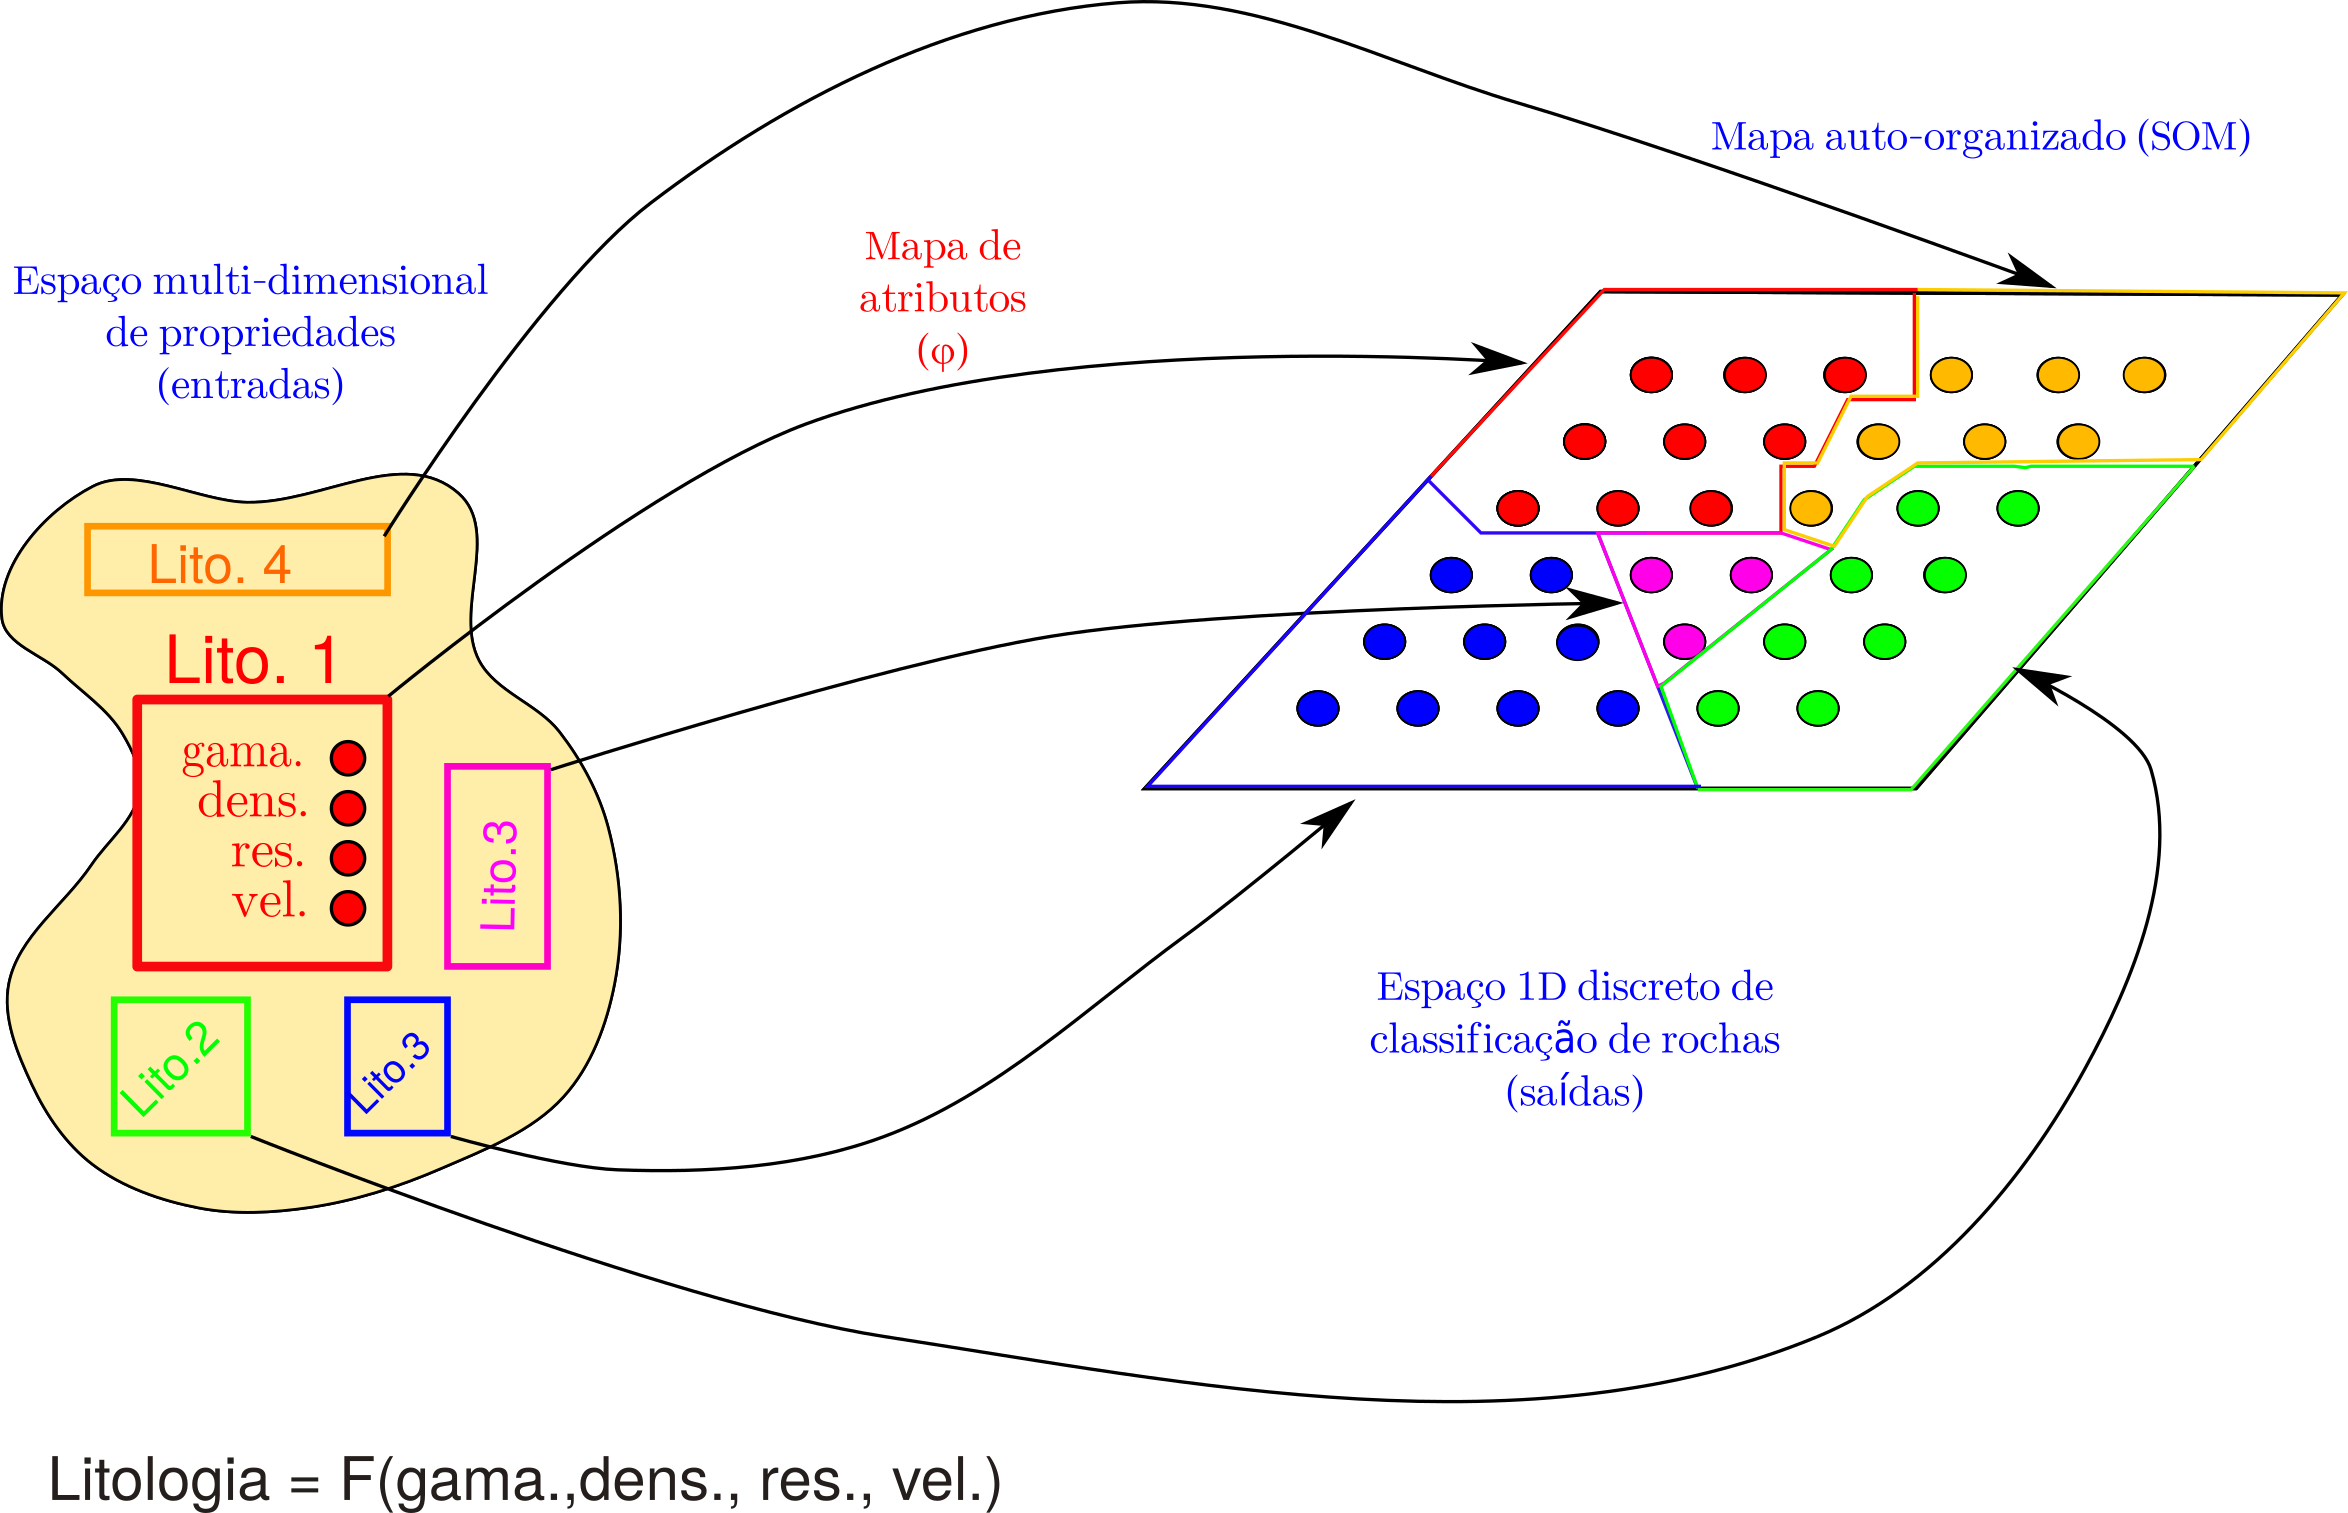
\includegraphics[scale=0.5]{Imagens/Introkoho4.png} 
\end{frame}

\begin{frame}
	\frametitle{Kohonen - SOM}
	\framesubtitle{Organização}
	
	\begin{eqnarray}
	\textbf{x}=[x_{1}, x_{2}, x_{3}, ..., x_{m}]^{T} \nonumber
	\end{eqnarray}
	\pause
	\begin{itemize}
		\centering
		\item[x], dado de entrada 
		\pause
	\end{itemize}
	\begin{eqnarray}
	\textbf{w}_{i,j}= [w_{j1}, w_{j2}, w_{j3}, ..., w_{jm}]^{T} \nonumber
	\end{eqnarray}
	\pause
	\begin{itemize}
		\centering
		\item[w], matriz de atributo neuronal 
	\end{itemize}
	\begin{eqnarray}
	j=1,2,3,\hdots,l \nonumber
	\end{eqnarray}
\end{frame}

%\begin{frame}
%    \frametitle{Kohonen - SOM}
%    \framesubtitle{Cooperation and winner neuron}
%	\begin{eqnarray}
%	i(\textbf{x})= argmin_{j}  \parallel \textbf{x} - \textbf{w}_{i,j} \parallel_{2} \nonumber
%	\end{eqnarray}
%%	 or 
%%	\begin{eqnarray}
%%	d(t)= \sqrt{\sum^{n}_{i=1}[x(t)-w_{i,j}(t)]^{2}} \hspace{1cm}  (j = {1,..,m}), \nonumber
%%	\label{eq1}
%%	\end{eqnarray}
%	
%	\begin{itemize}
%		\centering
%		\item[i(x)], distance or identity of a neuron i
%	\end{itemize}
%
%\end{frame}



\begin{frame}
	\frametitle{Kohonen - SOM}
	\framesubtitle{Processo de adaptação sináptica ou Treinamento}
	%Neuron changes the value of the surrounding neurons inside a quartet geometry
	%
	
	\begin{tcolorbox}[colback=gray!5,colframe=blue!40!black,title=Definição]
		\begin{equation}
		w_{i,j}(t+1)=w_{i,j}(t)+\eta(t)[x(t)-w_{i,j}(t)] \nonumber
		\label{eq2}
		\end{equation}  
	\end{tcolorbox}
	
	\pause
	
	\begin{itemize}
		\centering
		\item[$w_{i,j}(t+1)$],  atualização da matriz de atributos neuronais
		\item[$\eta(t)$], taxa de aprendizado
	\end{itemize}
	\pause
	\begin{tcolorbox}[colback=gray!5,colframe=blue!40!black,title=Definição]
		\begin{equation}
		\eta(t)=\eta(0)    ( 1 -  \frac{t}{T}  ) \nonumber
		\label{eq3}
		\end{equation}  
	\end{tcolorbox}
	
	\begin{itemize}
		\centering
		\item[$T$], número de ciclos de treinamento
		%	\pause
		\item[$t$], número de iterações
		%\pause
		%\item A iteractive process $t=t+1$ goes on until $t \approx  T$. Once the process ends for one neuron it repeats it self for the surrounding neighbors \citep{YANG2009,Yan2014}.
	\end{itemize}
	
	%Where $T$ is the number of training cyles and $t$ is the number of iteractions. A iteractive process $t=t+1$ goes on until $t \approx  T$. Once the process ends for one neuron it repeats it self for the surrounding neighbors.
	
\end{frame}


\begin{frame}
	\frametitle{A geometria da rede}
	
	\begin{columns}
		\column{0.2\textwidth}
		\begin{figure}[H]
			\flushleft
			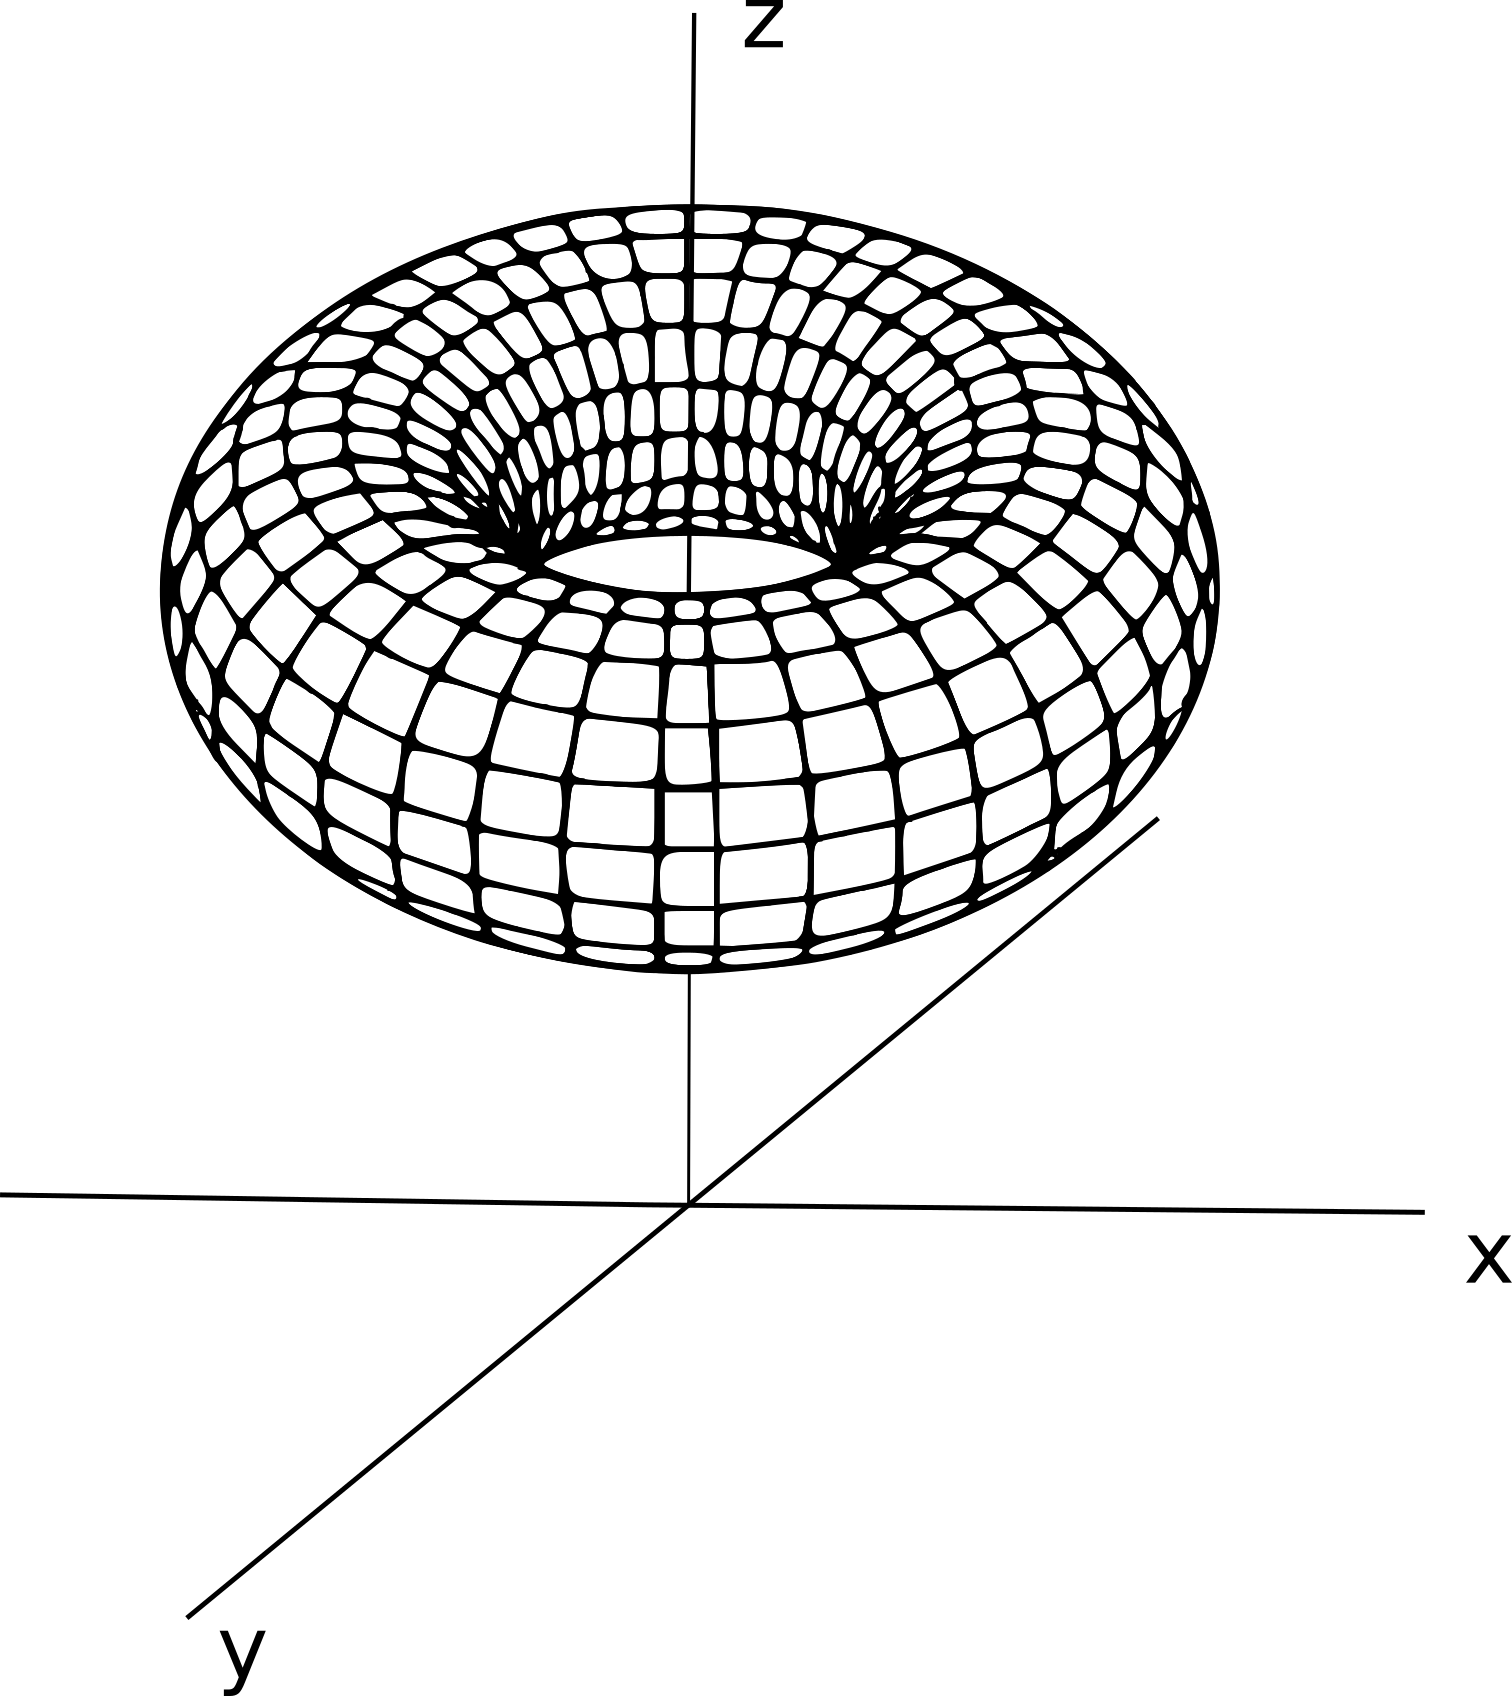
\includegraphics[scale=0.2]{Imagens/toro.png}
			\label{toro}
		\end{figure}
		\column{0.5\textwidth}
		\begin{figure}
			\flushright
			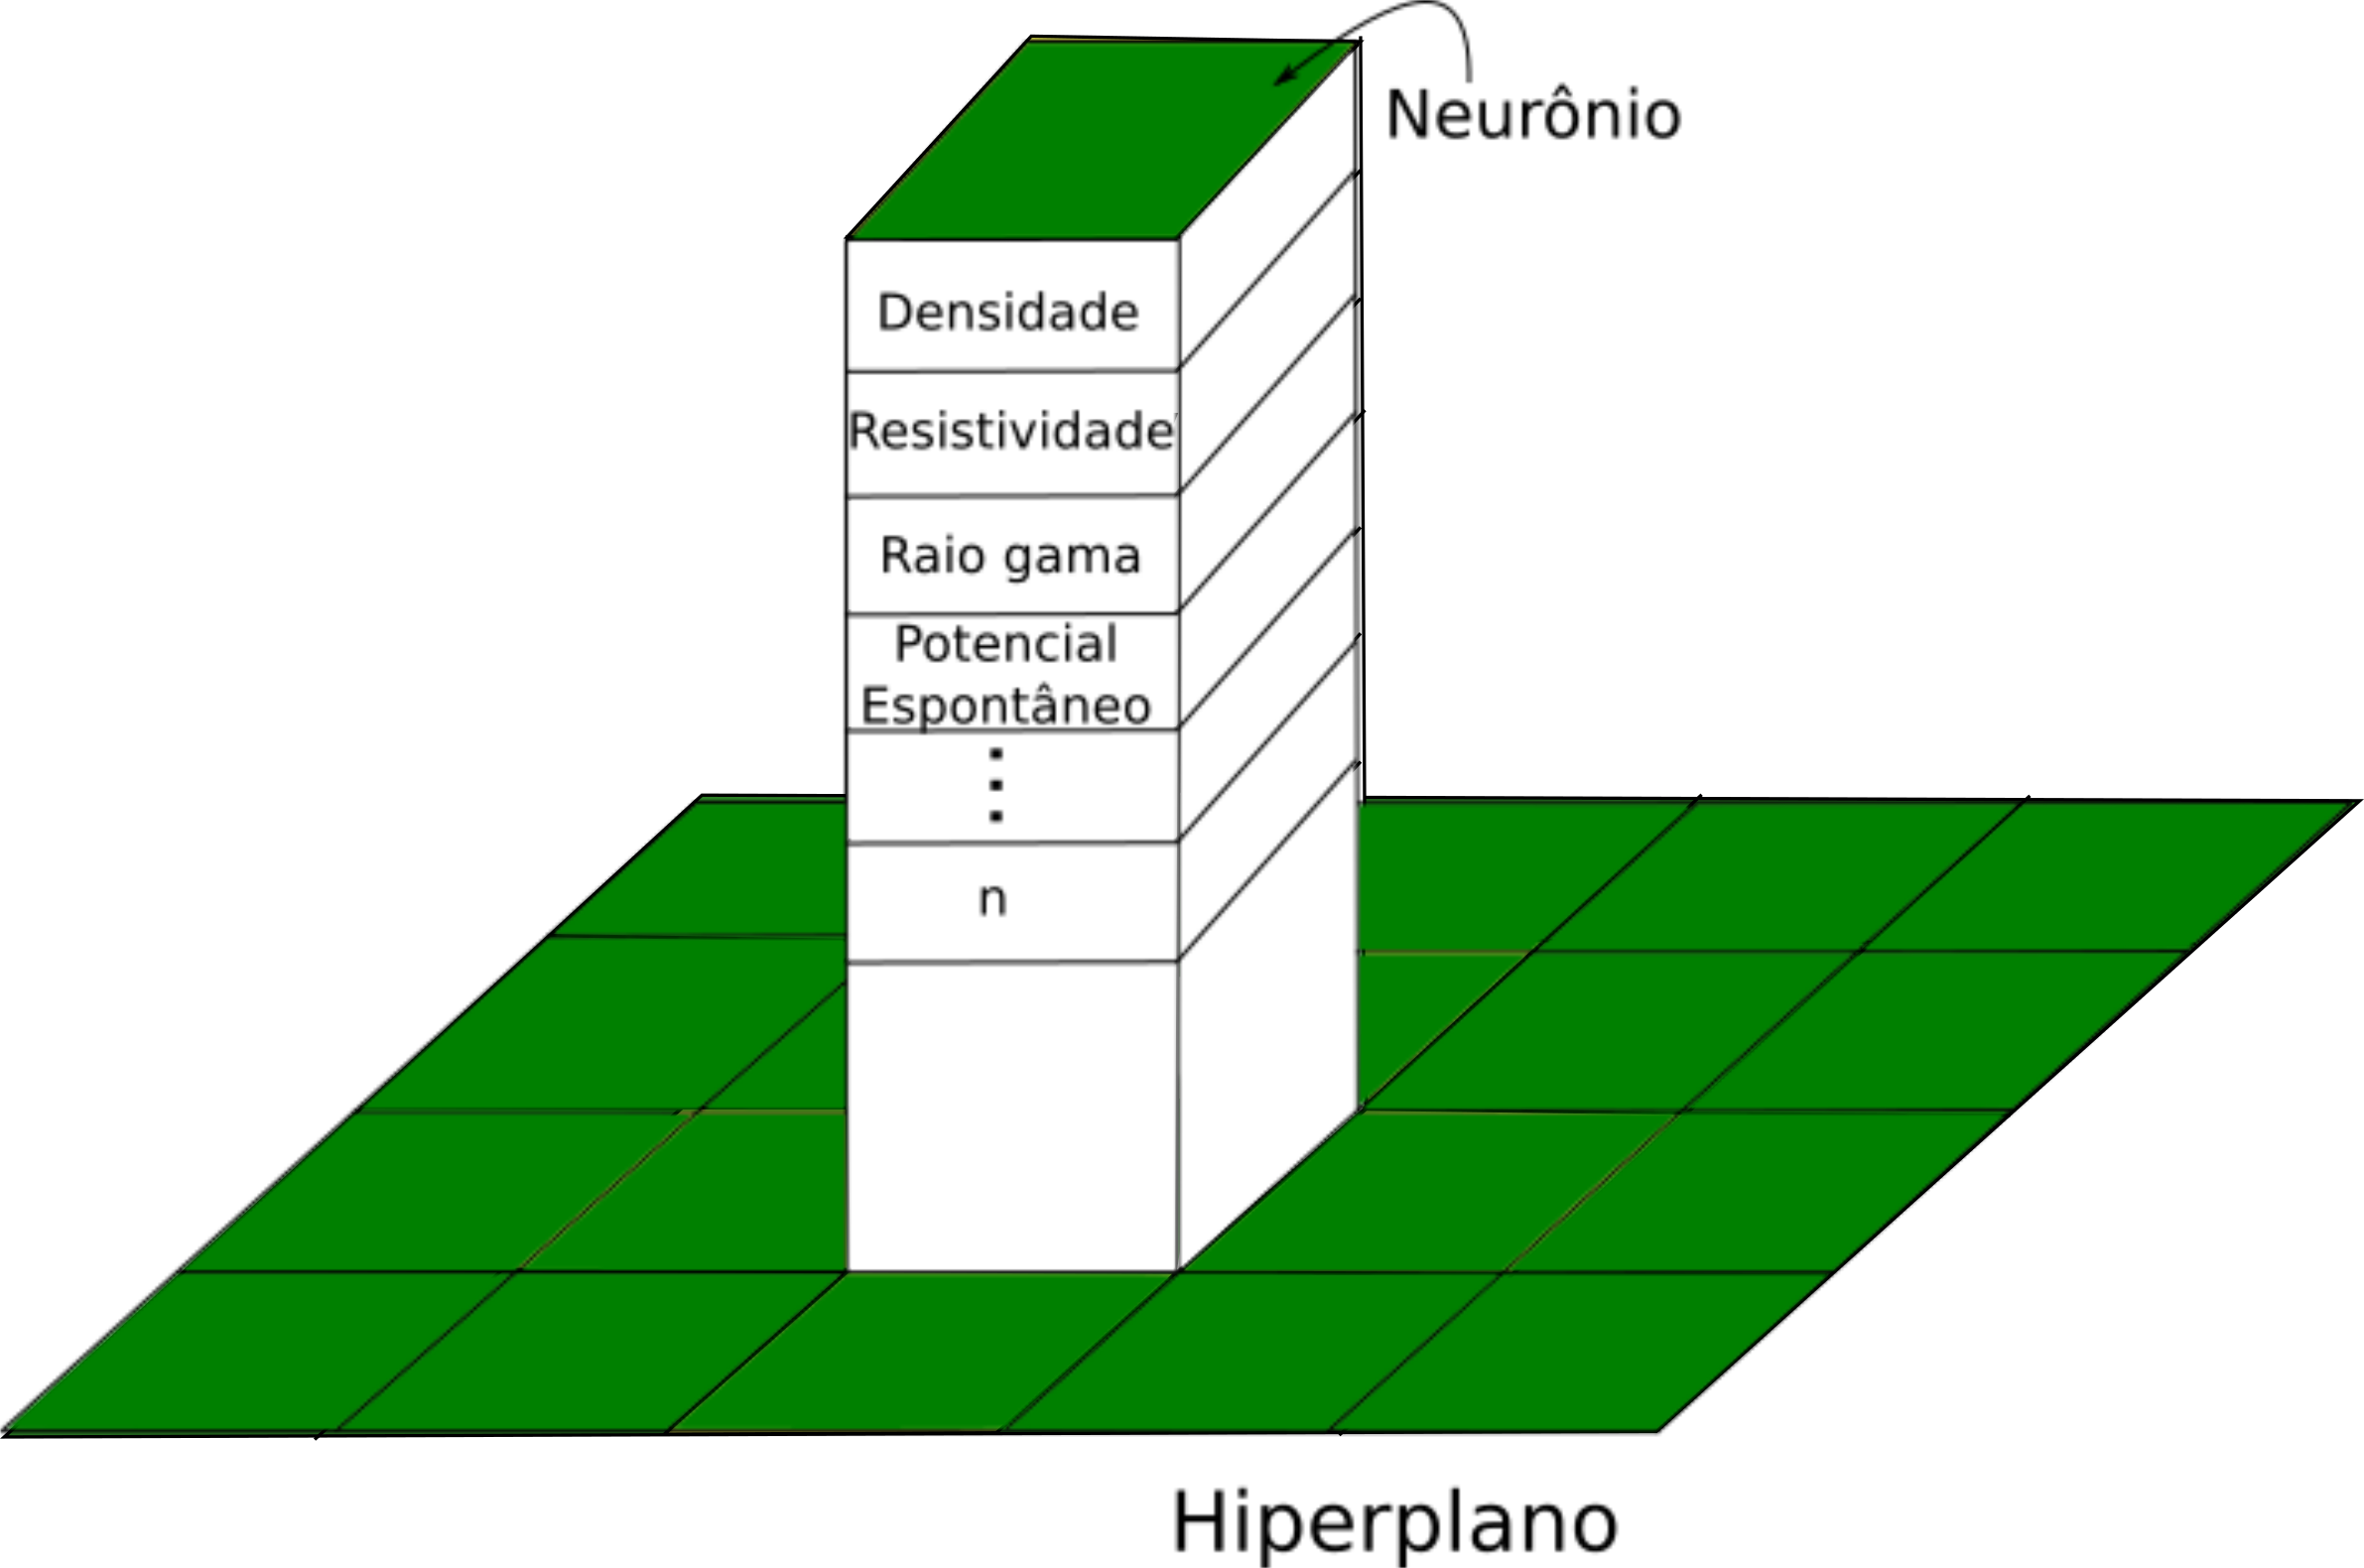
\includegraphics[scale=0.3]{Imagens/hiperplano.png}
			\label{hiperplano}
		\end{figure}
	\end{columns}
	\pause
	\begin{itemize}
		\footnotesize
		\centering
		\item[Toroide], é uma forma eficiente de conetar todos os neurônios
		\item[Hiperplano], aonde localizam-se as informações dos atributos
	\end{itemize}
\end{frame}


\begin{frame}
	\frametitle{Neurônio vencedor e a vizinhança}	
	\begin{eqnarray}
	i(\textbf{x})= argmin \parallel \textbf{x} - \textbf{w}_{i,j} \parallel_{2} \nonumber
	\end{eqnarray}
	\begin{figure}
		\centering
		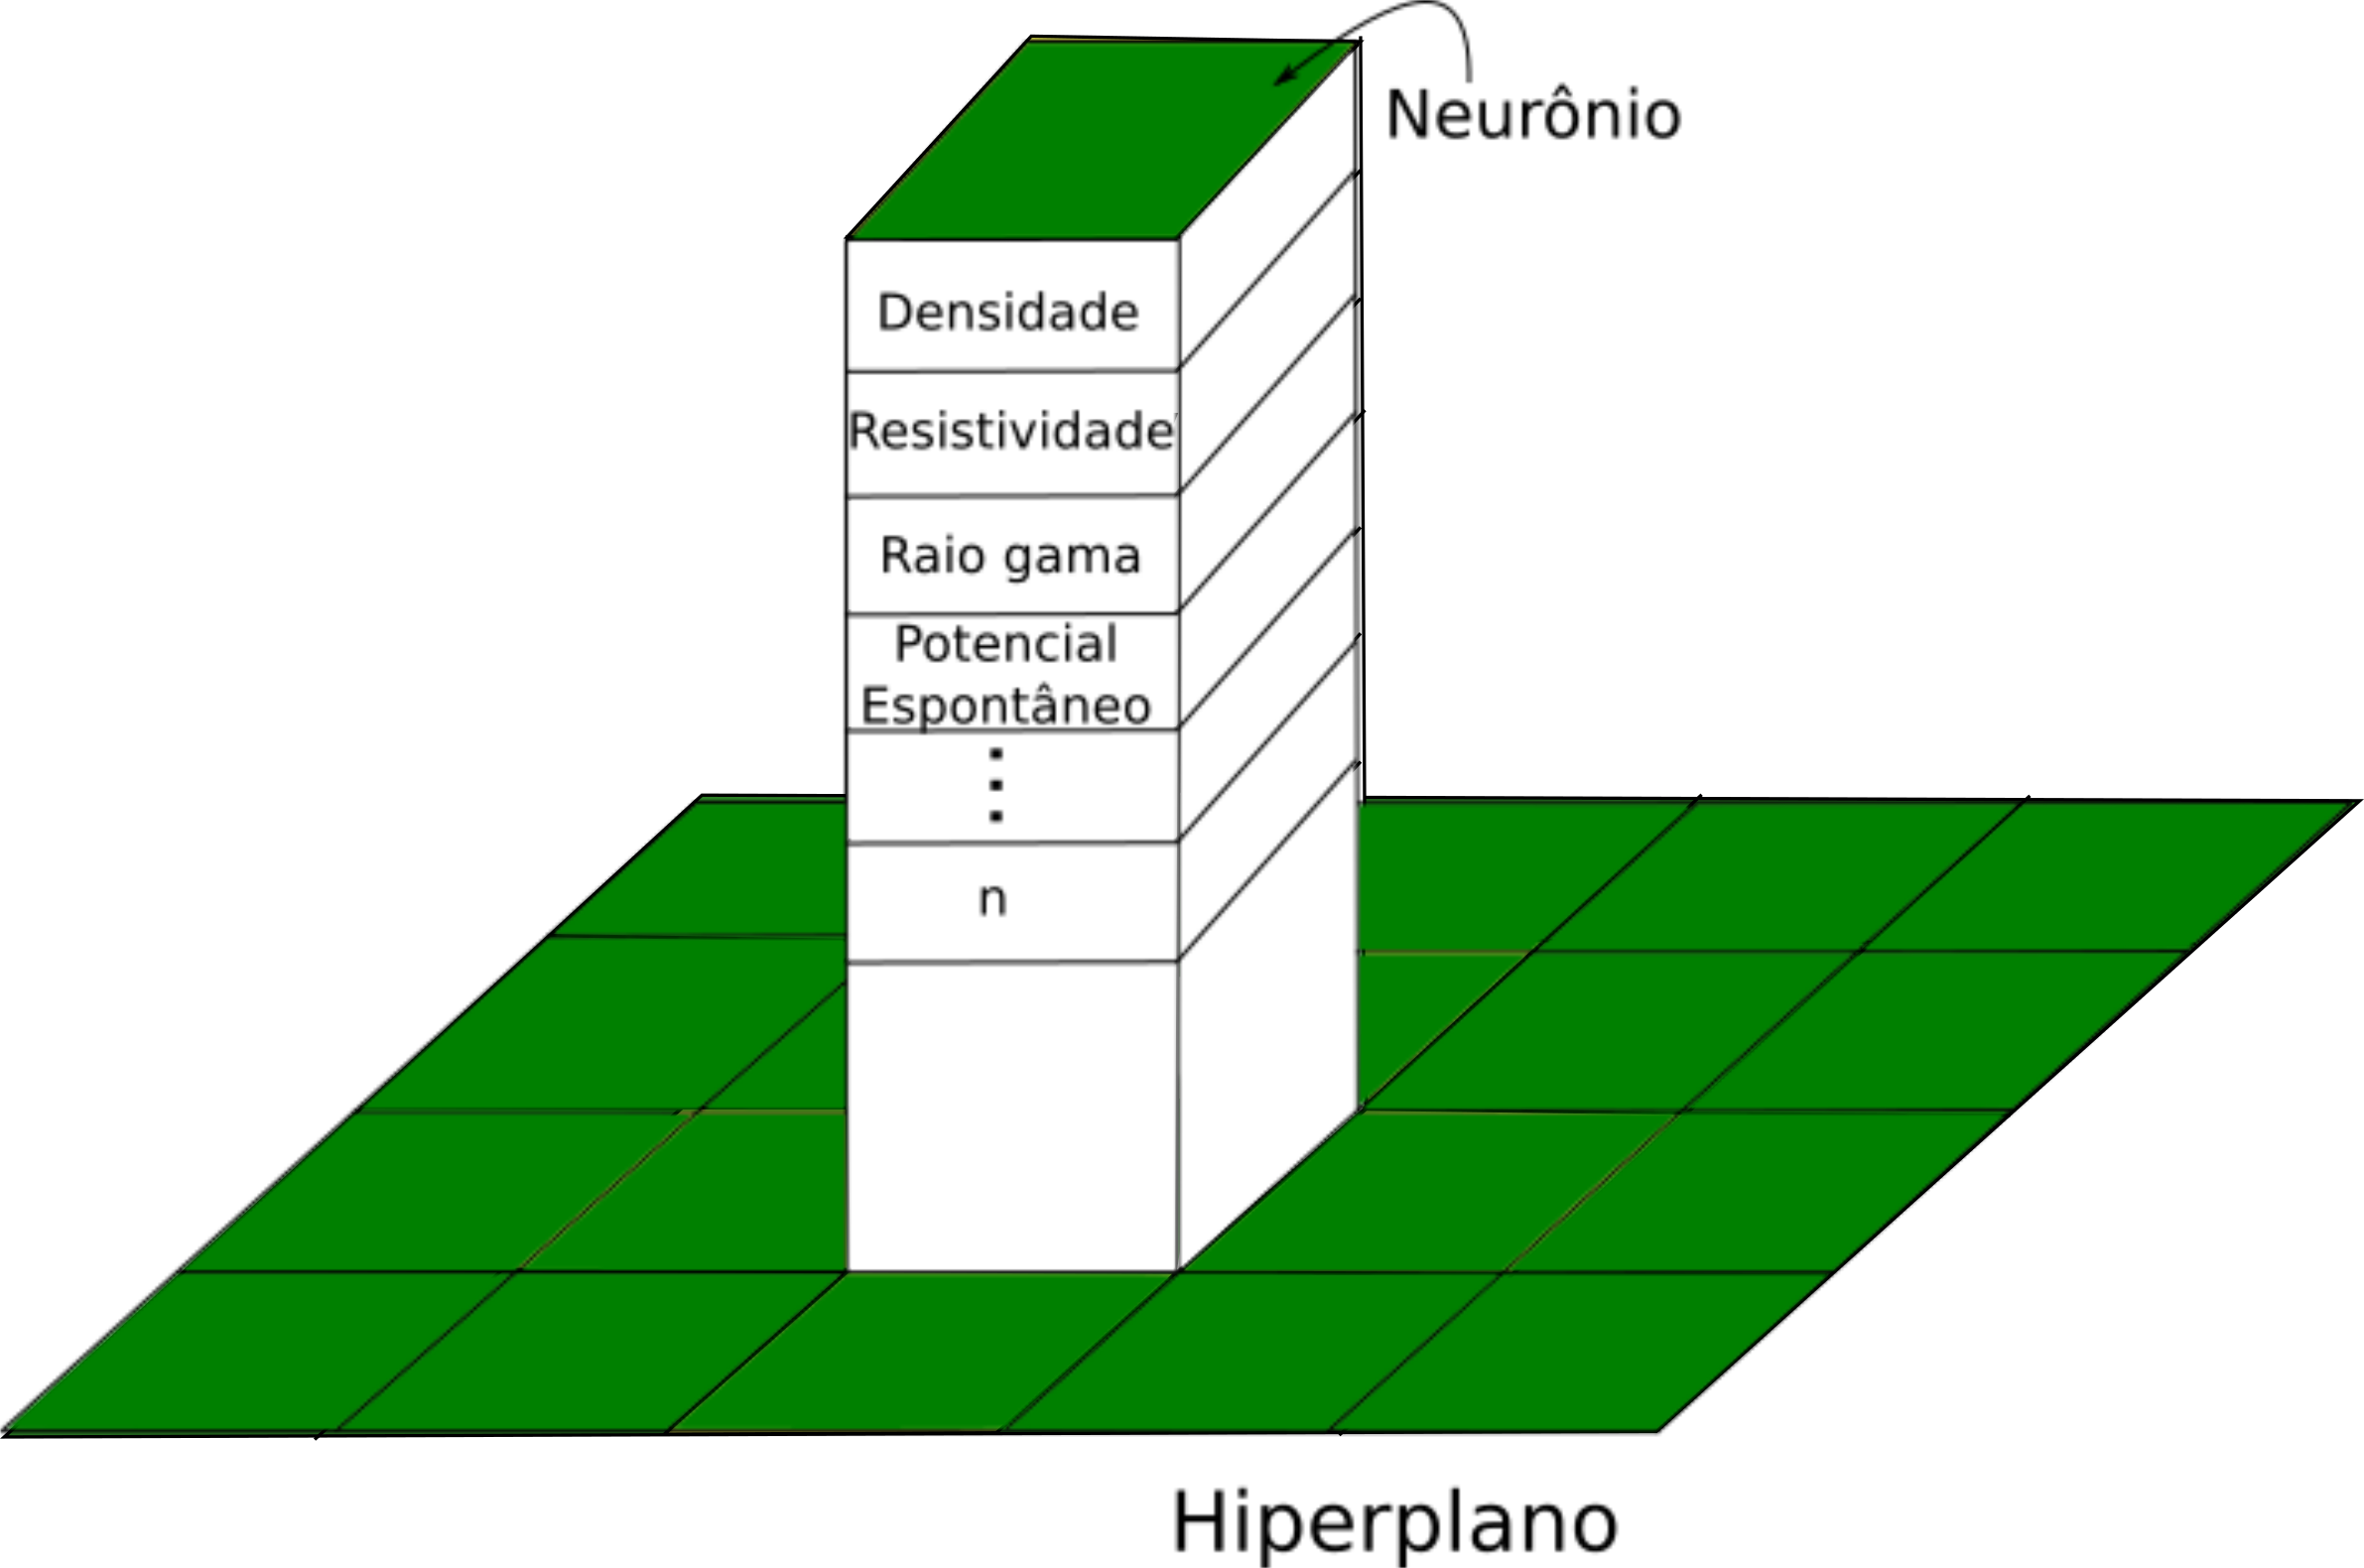
\includegraphics[scale=0.33]{Imagens/hiperplano.png}
		\label{vencedor1}
	\end{figure}
\end{frame}

\begin{frame}
	\frametitle{Neurônio vencedor e a vizinhança}
	\begin{eqnarray}
	i(\textbf{x})= argmin  \parallel \textbf{x} - \textbf{w}_{i,j} \parallel_{2} \nonumber
	\end{eqnarray}
	\begin{figure}
		\centering
		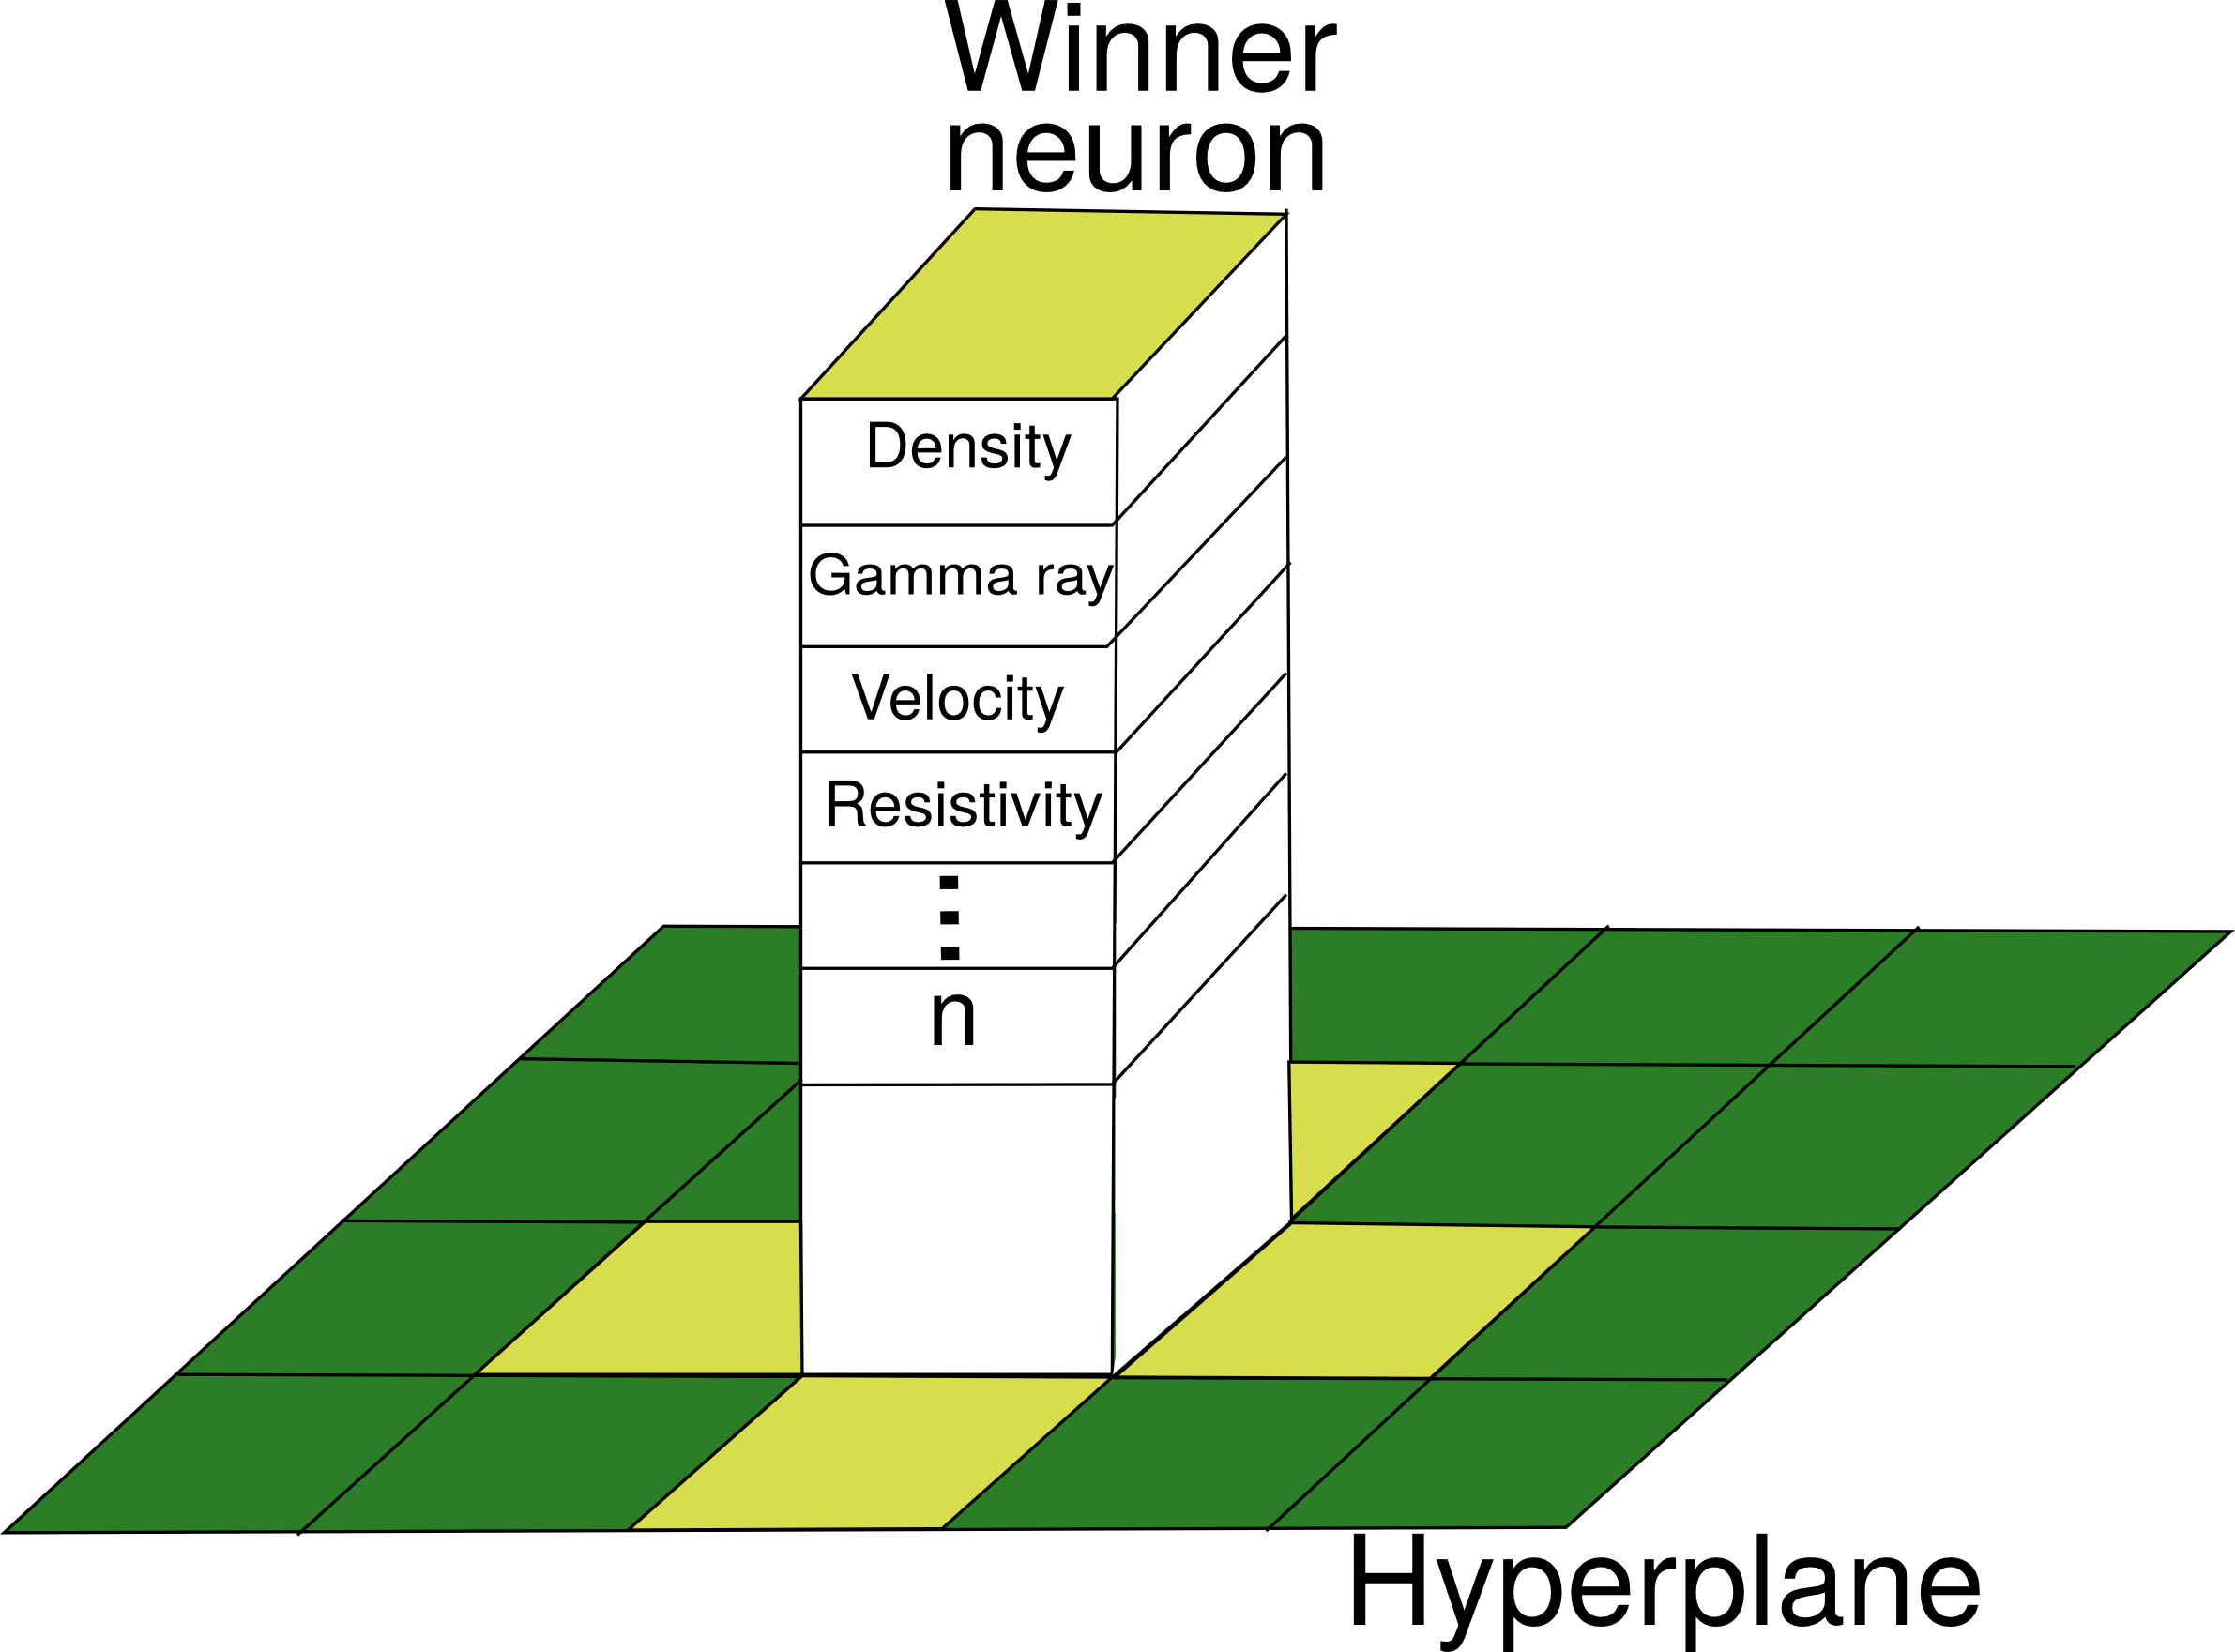
\includegraphics[scale=0.33]{Imagens/winner.png}
	\end{figure}
\end{frame}

\begin{frame}
	\frametitle{Neurônio vencedor e a vizinhança}
	\begin{eqnarray}
     \textcolor{yellow}{v}(\textbf{w}_{i+1,j}, \textbf{w}_{i-1,j}, \textbf{w}_{i,j+1}, \textbf{w}_{i-1,j})  \nonumber
	\end{eqnarray}
	\begin{figure}
		\centering
		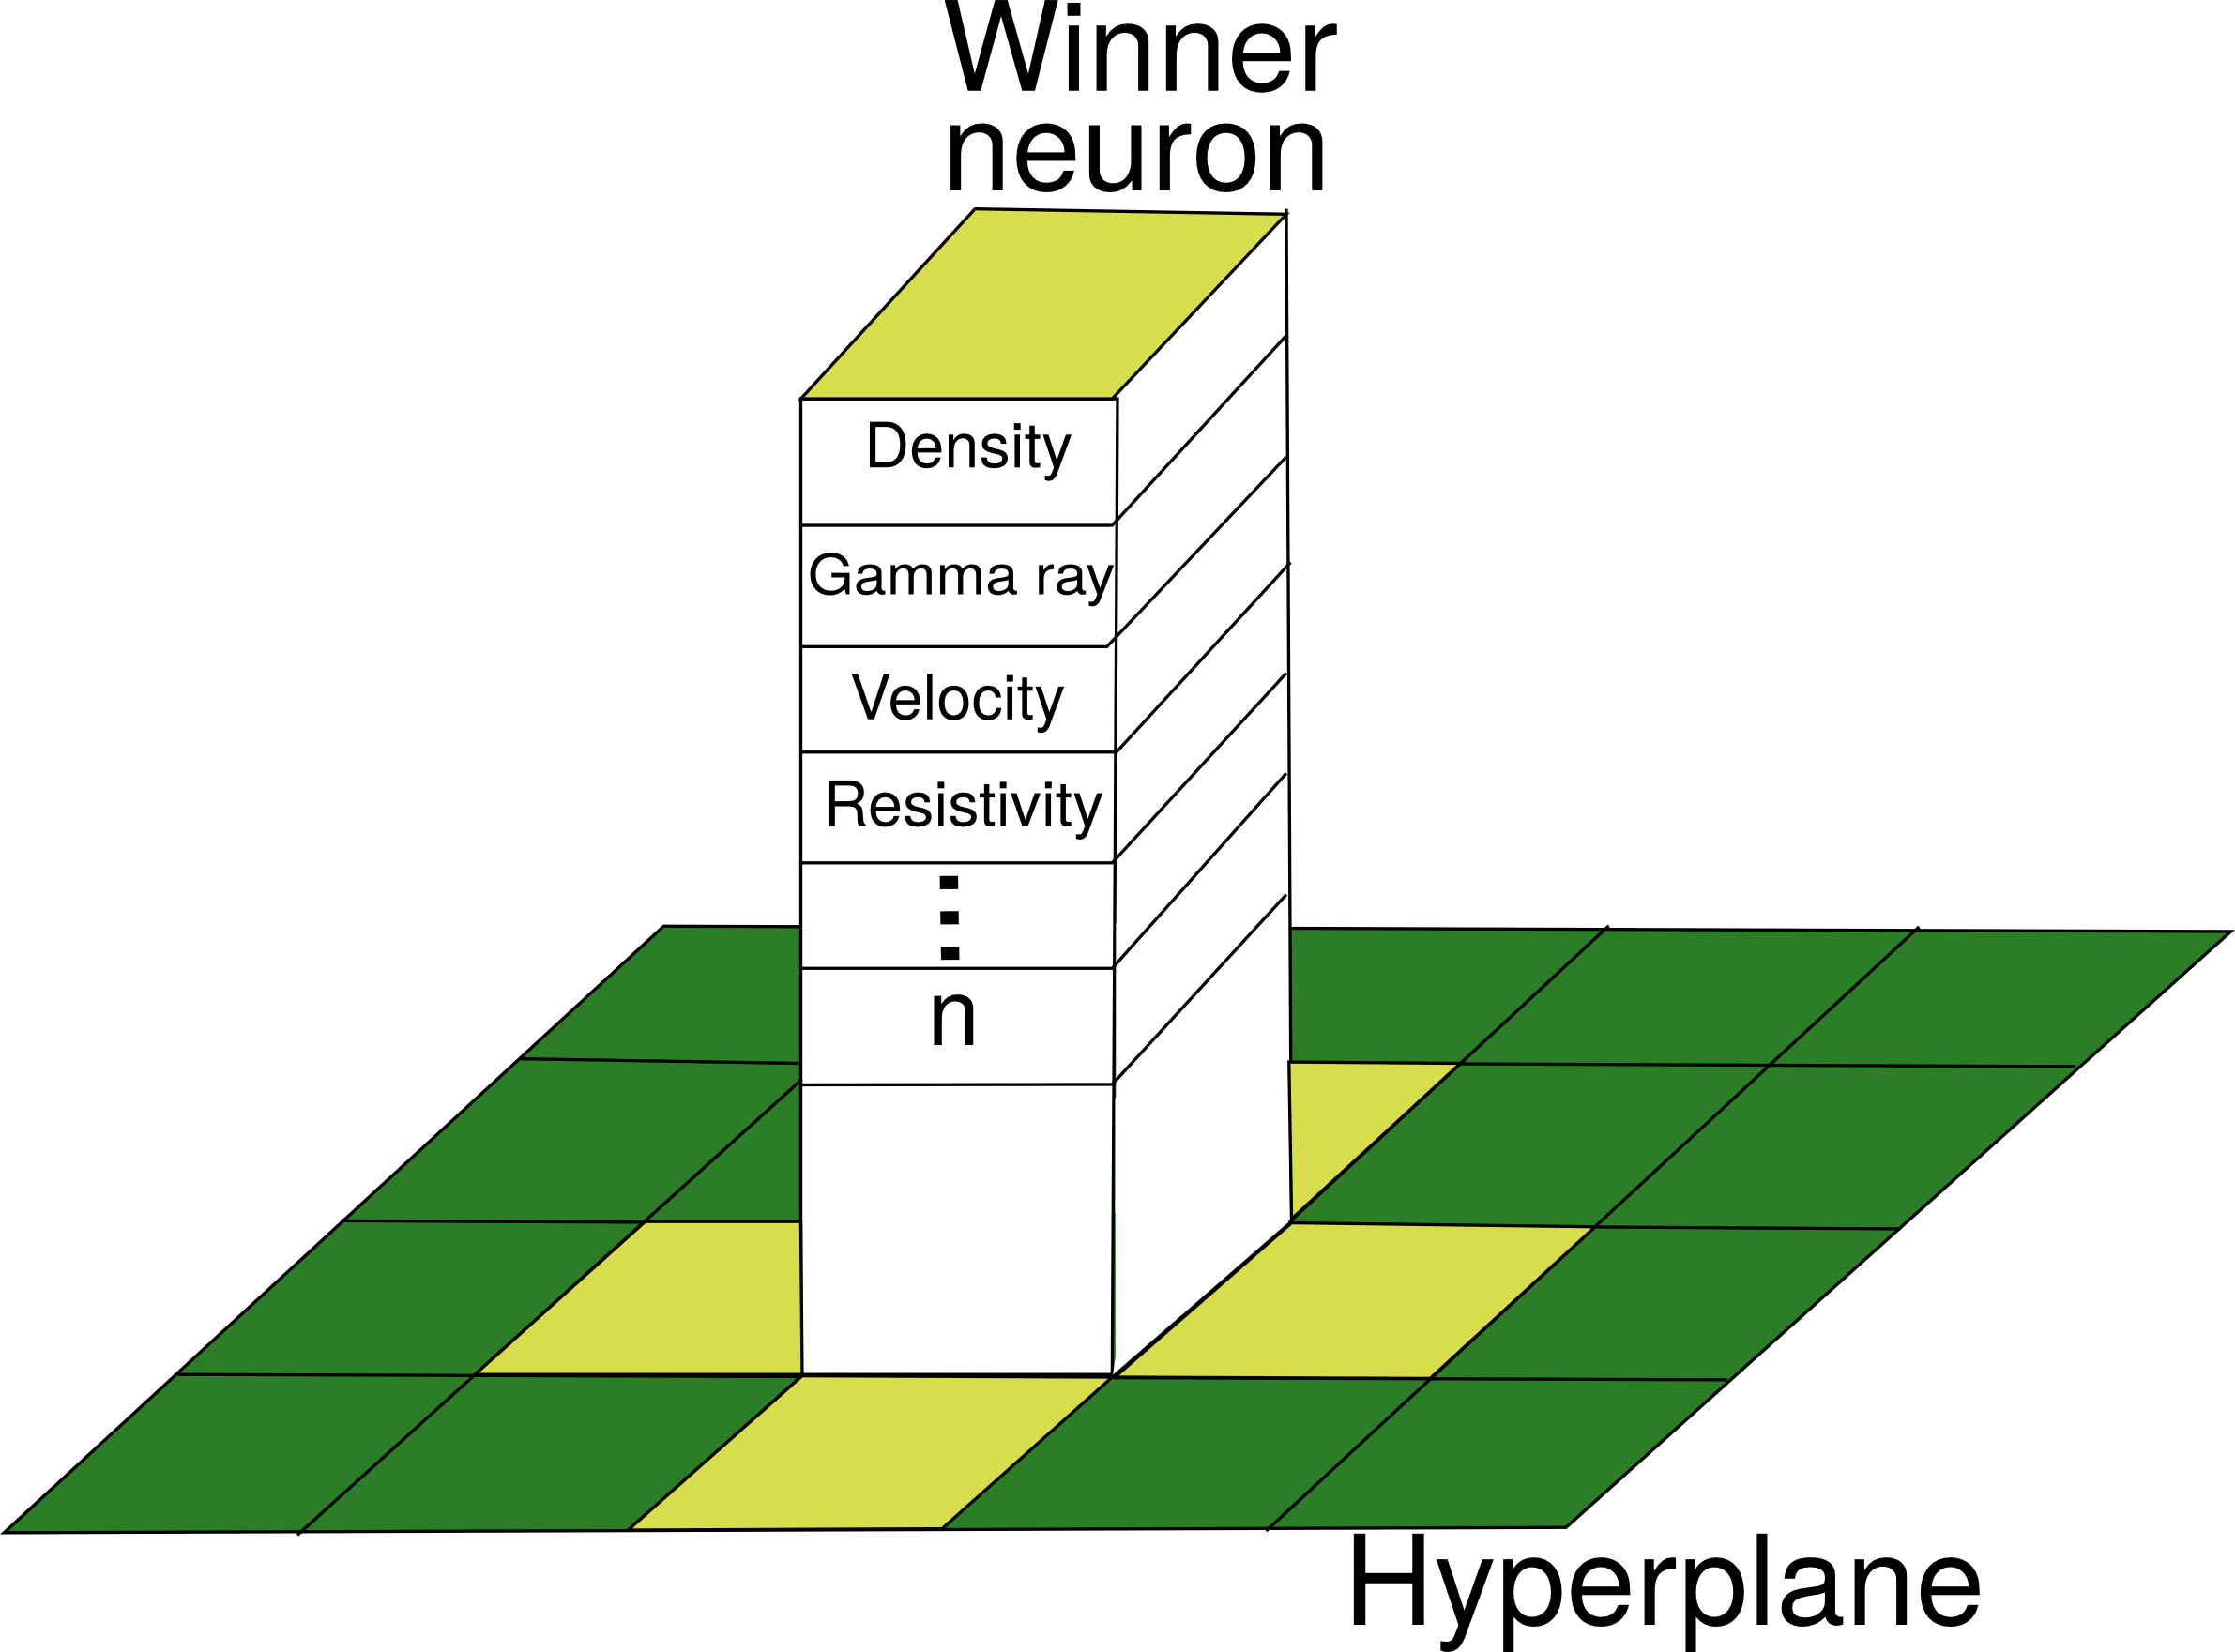
\includegraphics[scale=0.33]{Imagens/winner.png}
	\end{figure}
\end{frame}

\subsection{O programa da Rede}

%\subsection{Fluxograma de criação dos dados sintéticos}
\begin{frame}
	\frametitle{Fluxograma de criação dos dados sintéticos}
	\begin{footnotesize}
		\begin{figure}[H]
			\centering
			
			\begin{tikzpicture}
			[node distance=.5cm,
			start chain=going below,]
			\node[punktchain, join]  {Modelo de Bacia};
			\node[punktchain, join]   {Dados da Literatura};
			\node[punktchain, join]   {Estimar erros das propriedades físicas para dada litologia};
			\node[punktchain, join] {Definir taxa de amostragem};
			\node[punktchain, join, ] {Gerar dados sintéticos contaminados com o erro gaussiano estimado};
			
			\end{tikzpicture}
			%		\caption{Fluxograma do programa de geração dos dados sintéticos}
		\end{figure}
		
	\end{footnotesize}	
\end{frame}

%\subsection{Fluxograma de Treinamento da rede}
\begin{frame}
	\frametitle{Fluxograma de treinamento}
	\begin{scriptsize}
		
		
		\begin{figure}[H]
			\centering
			
			%		\begin{tikzpicture}
			%		[node distance=.3cm,
			%		start chain=going below,]
			%		\node[punktchain, join]  {Início};
			%		\node[punktchain, join] (L1)  {Entrar com os dados do treinamento};
			%		\node[punktchain, join]   {Atualizar o peso do neurônio vencedor};
			%		\node[punktchain, join] (L2) {Fazer alteração nas vizinhanças do neurônio vencedor. Varre os dados de forma sequencial};
			%		\node[punktchain, join, ] {Avaliar o nível de treinamento da rede};
			%		\node[punktchain, join, ] {\color{red}Caso não esteja satisfatório volta-se para o Início e repete o processo de forma acumulativa};
			%		\node[punktchain, join, ] {\color{blue}Caso esteja satisfatório é o decretado o final do treinamento};	
			%		\end{tikzpicture}
			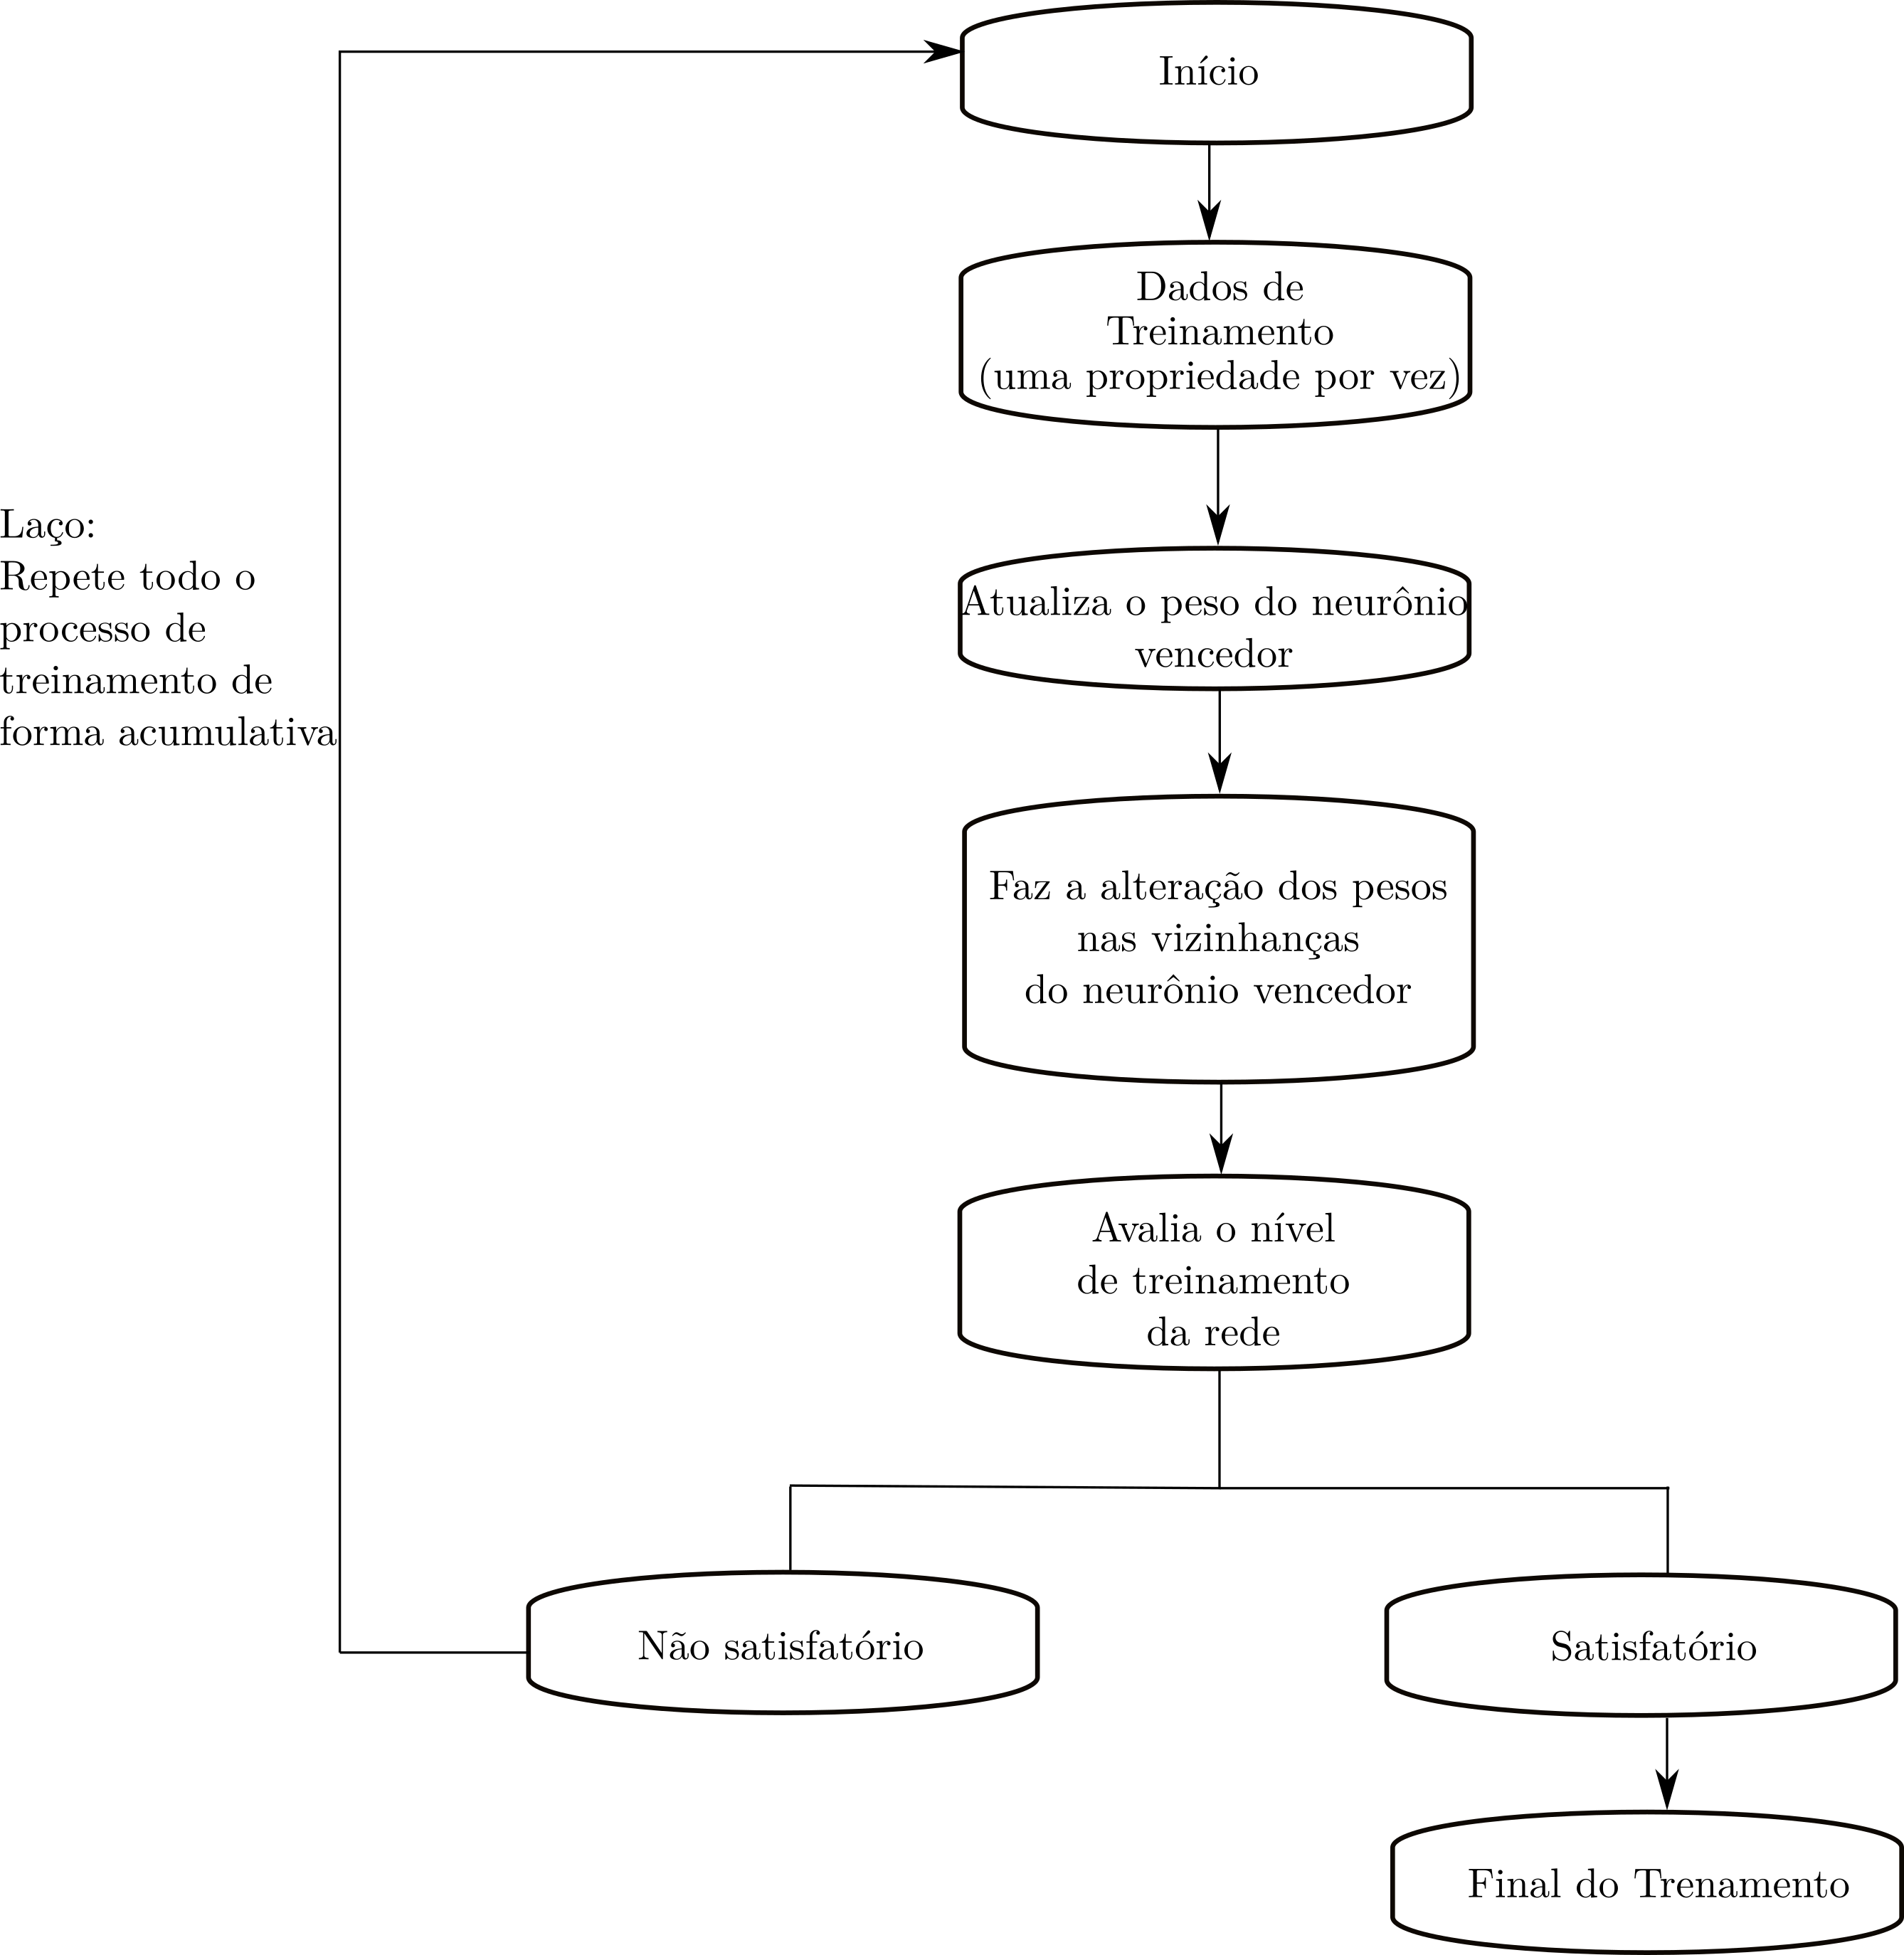
\includegraphics[scale=0.35]{Imagens/treinamento.png}
		\end{figure}
	\end{scriptsize}
\end{frame}


%\subsection{Fluxograma de classificação da rede}
\begin{frame}
	\frametitle{Fluxograma de classificação}
	\begin{small}
		
		
		\begin{figure}[H]
			\centering
			
			\begin{tikzpicture}
			[node distance=.8cm,
			start chain=going below,]
			\node[punktchain, join]  {Entrada do dado não classificado};
			\node[punktchain, join] (L1)  {Determina a distância entre o dado e os valores dos neurônios da rede};
			\node[punktchain, join]   {Armazena as distâncias};
			\node[punktchain, join] (L2) {Seleciona a menor distância};
			\node[punktchain, join, ] {Classifica o dado};	
			\end{tikzpicture}
			
			%		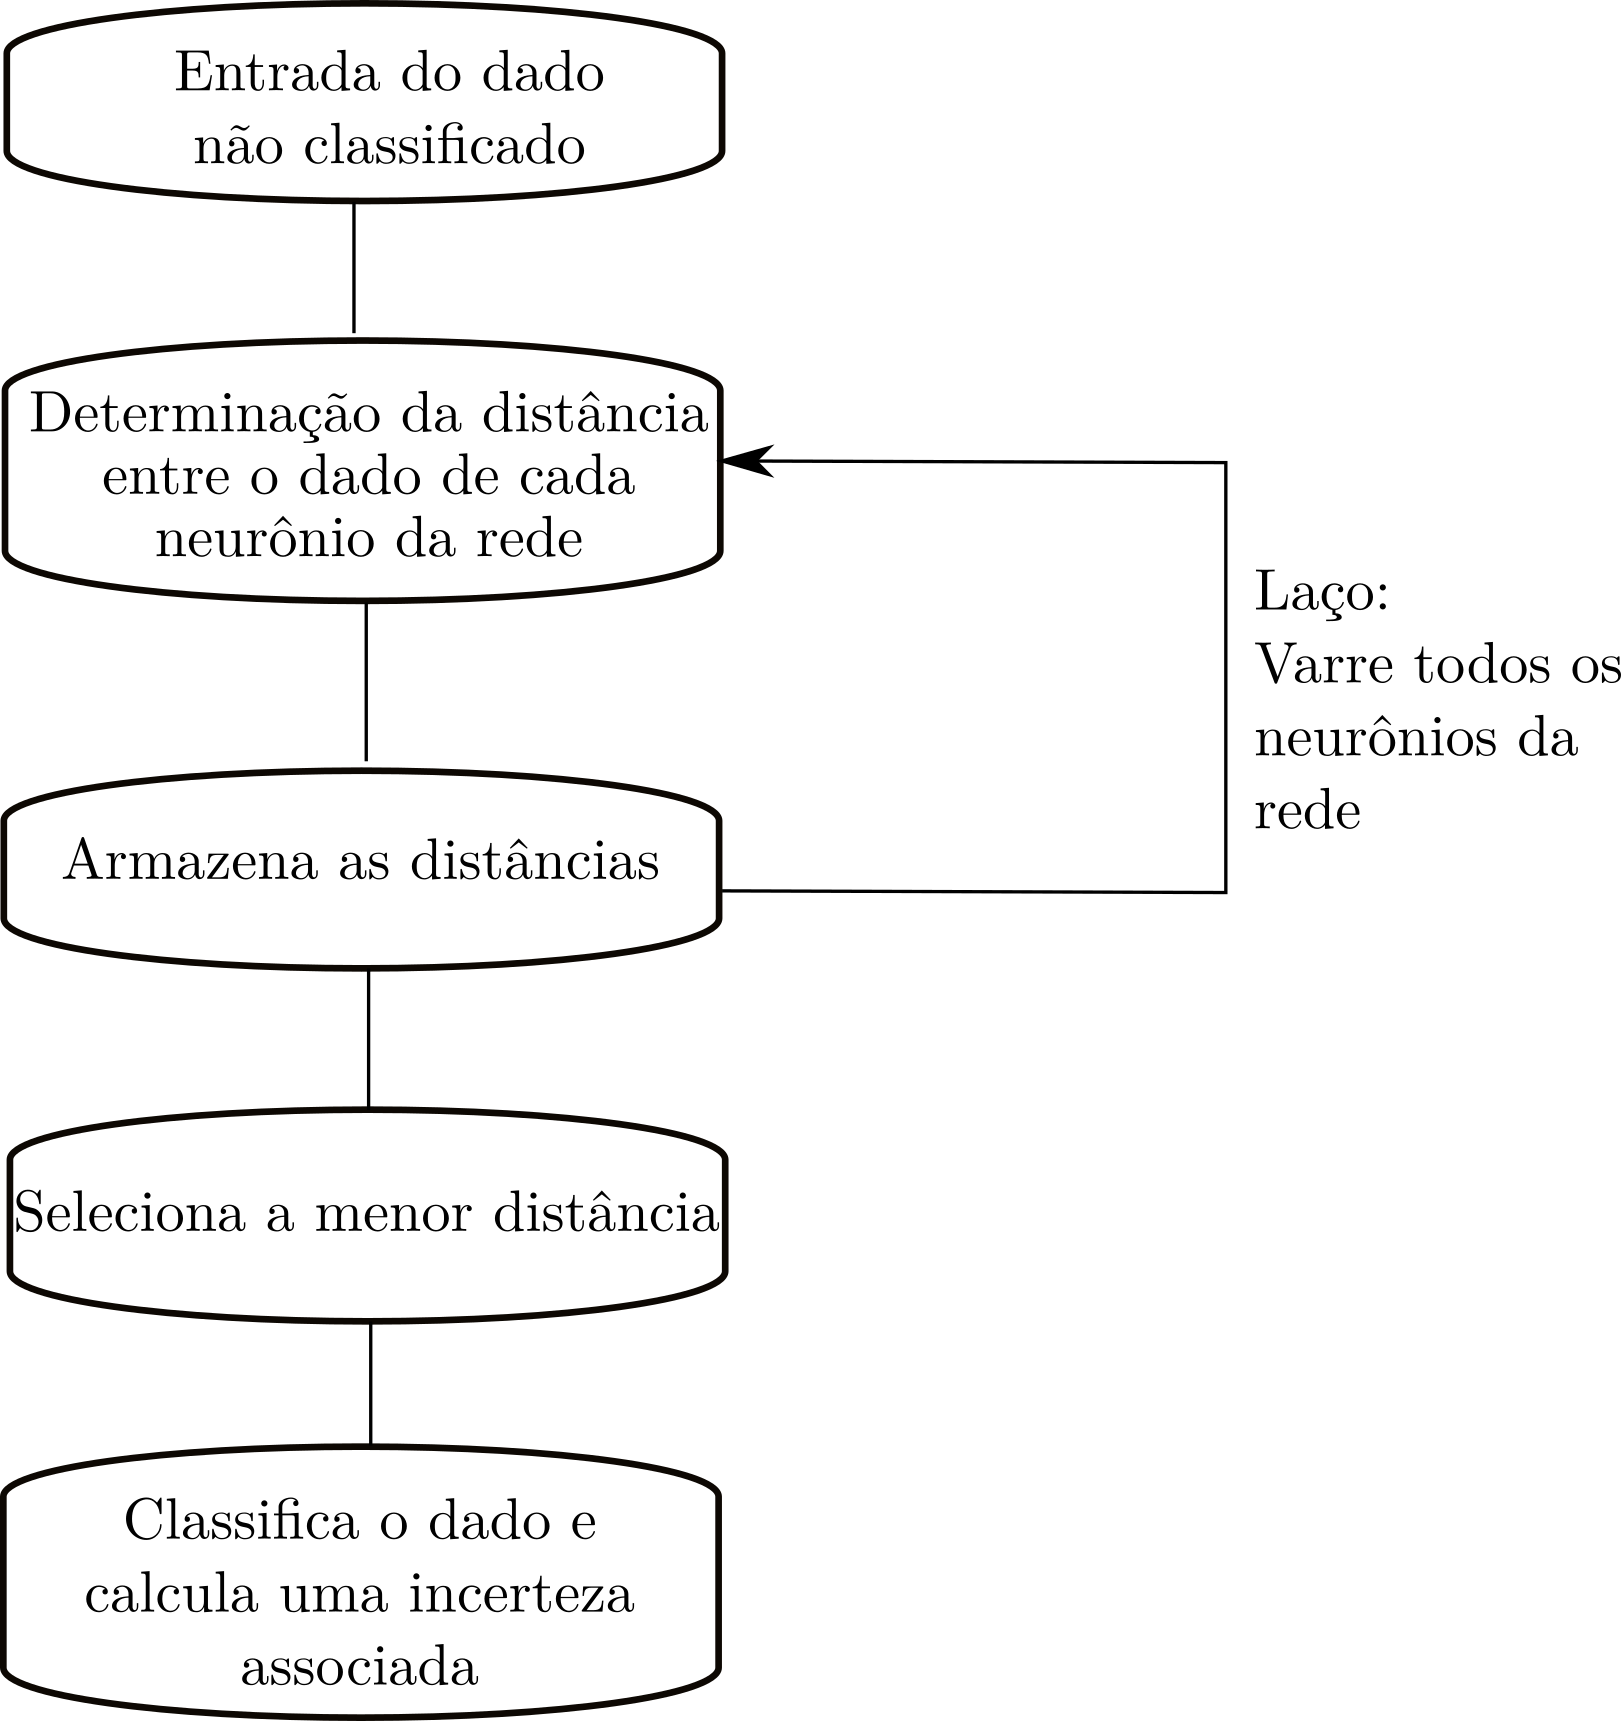
\includegraphics[scale=0.55]{Imagens/classificacao.png}
		\end{figure}
	\end{small}
\end{frame}




%%%%%%%%%%%%%%%%%%%%%%%%%%%%%%%%%%%%%%%%%%%%%%%%%%%%%%%%%%%%%%%%%%%%%%%%%%%%
%-------------------------RESULTADOS E DISCUSSÕES---------------------------------------
%%%%%%%%%%%%%%%%%%%%%%%%%%%%%%%%%%%%%%%%%%%%%%%%%%%%%%%%%%%%%%%%%%%%%%%%%%%%

\section{Resultados e Discussões}

\subsection{Dado Sintético}

\begin{frame}
\frametitle{Treinamento}
\begin{figure}
\centering
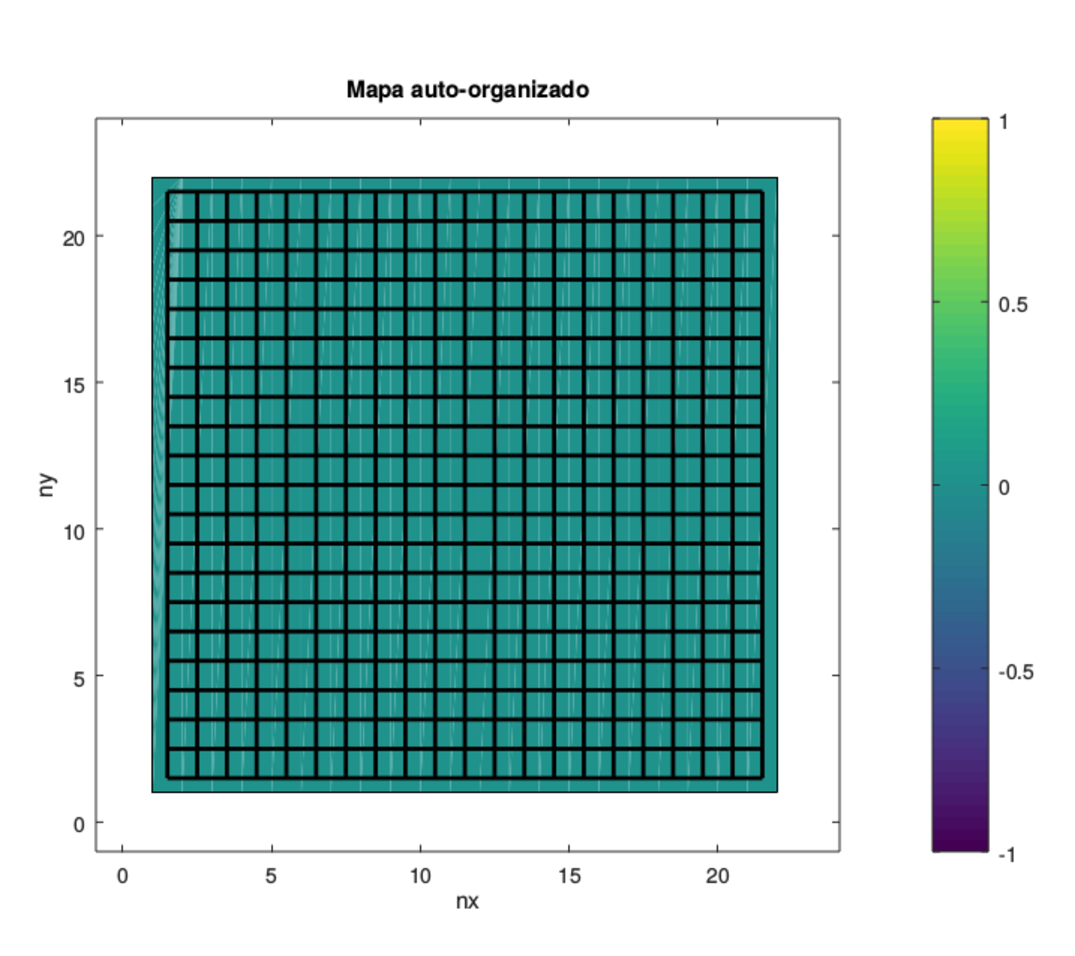
\includegraphics[width=7.0cm]{Imagens/SOM1_2d.pdf}
\caption{Mapa auto-organizado (a) no primeiro ciclo de treinamento.}
\end{figure}
\end{frame}

\begin{frame}
\frametitle{Treinamento}
\begin{figure}
\centering
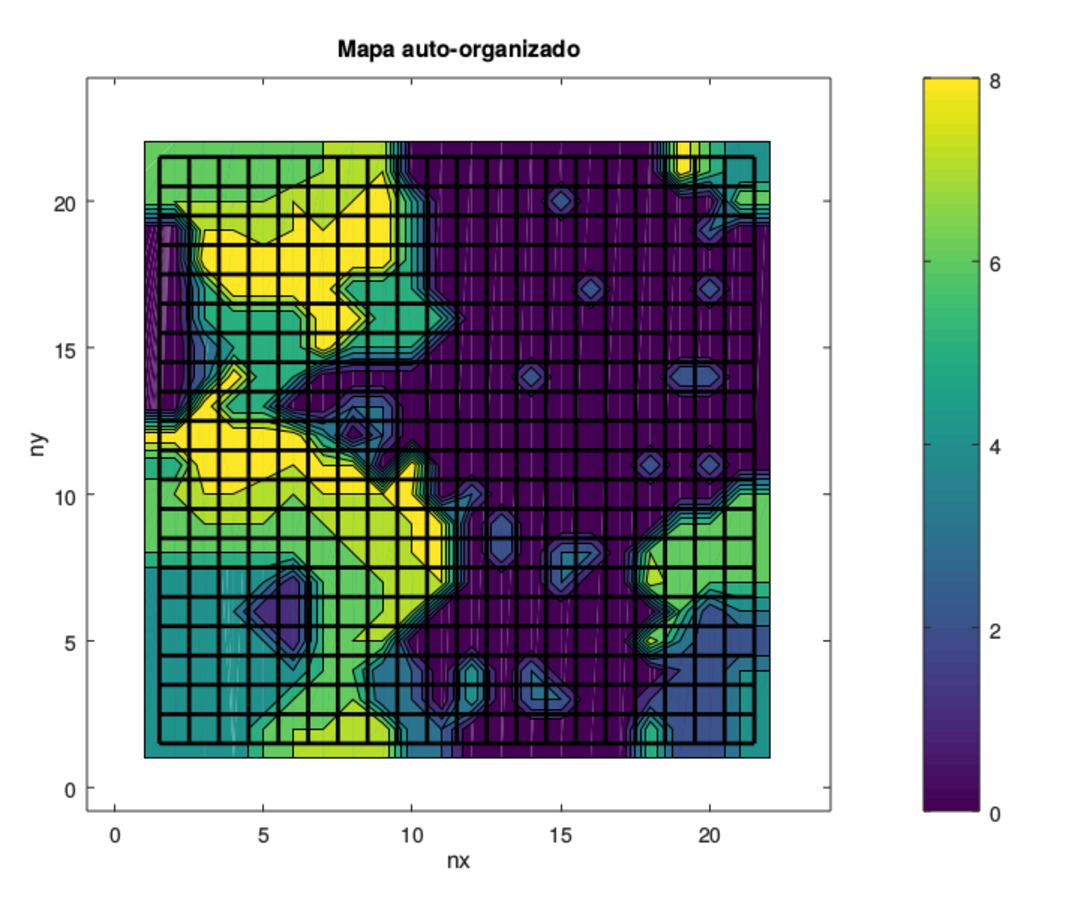
\includegraphics[width=7.0cm]{Imagens/SOM5_2d.pdf}
\caption{Mapa auto-organizado (b) no quinto ciclo de treinamento.}
\end{figure}
\end{frame}

\begin{frame}
\frametitle{Treinamento}
\begin{figure}
\centering
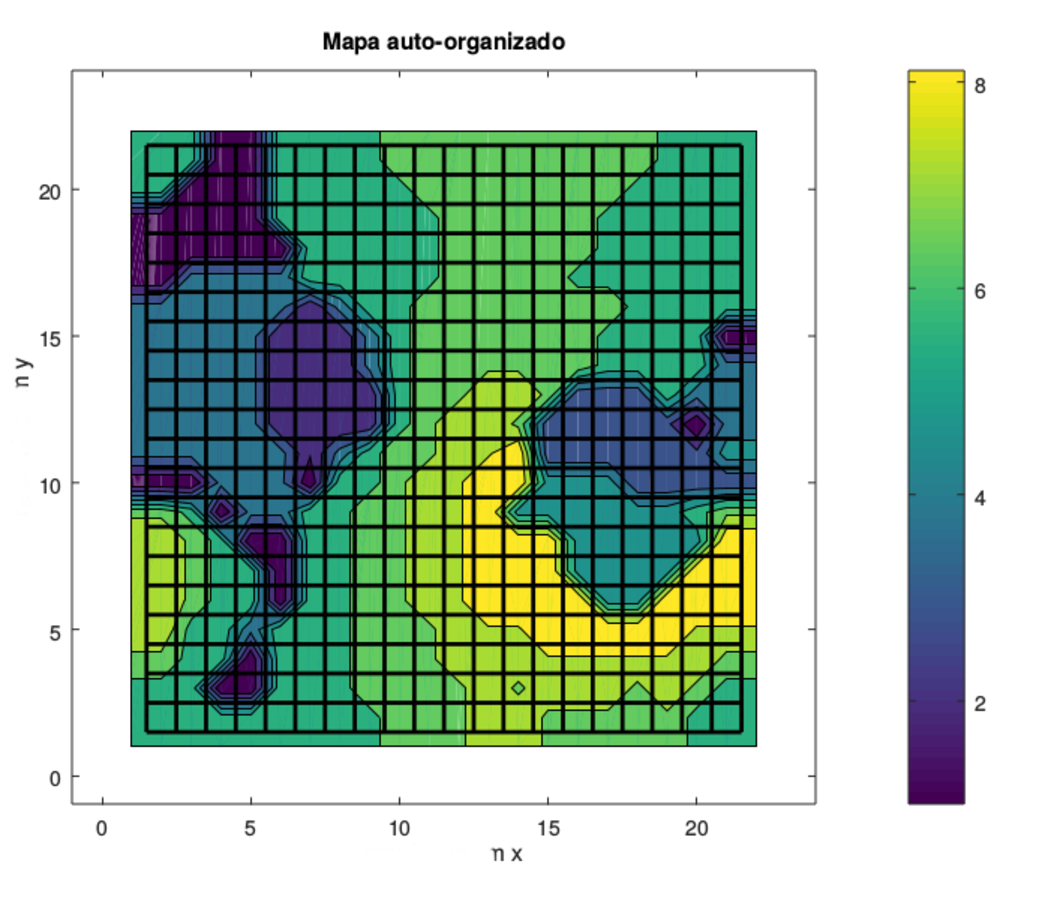
\includegraphics[width=7.0cm]{Imagens/SOM100_2d.pdf}
\caption{Mapa auto-organizado (c) no centésimo ciclo de treinamento.}
\end{figure}
\end{frame}

\begin{frame}
\frametitle{Treinamento}
\begin{figure}
\centering
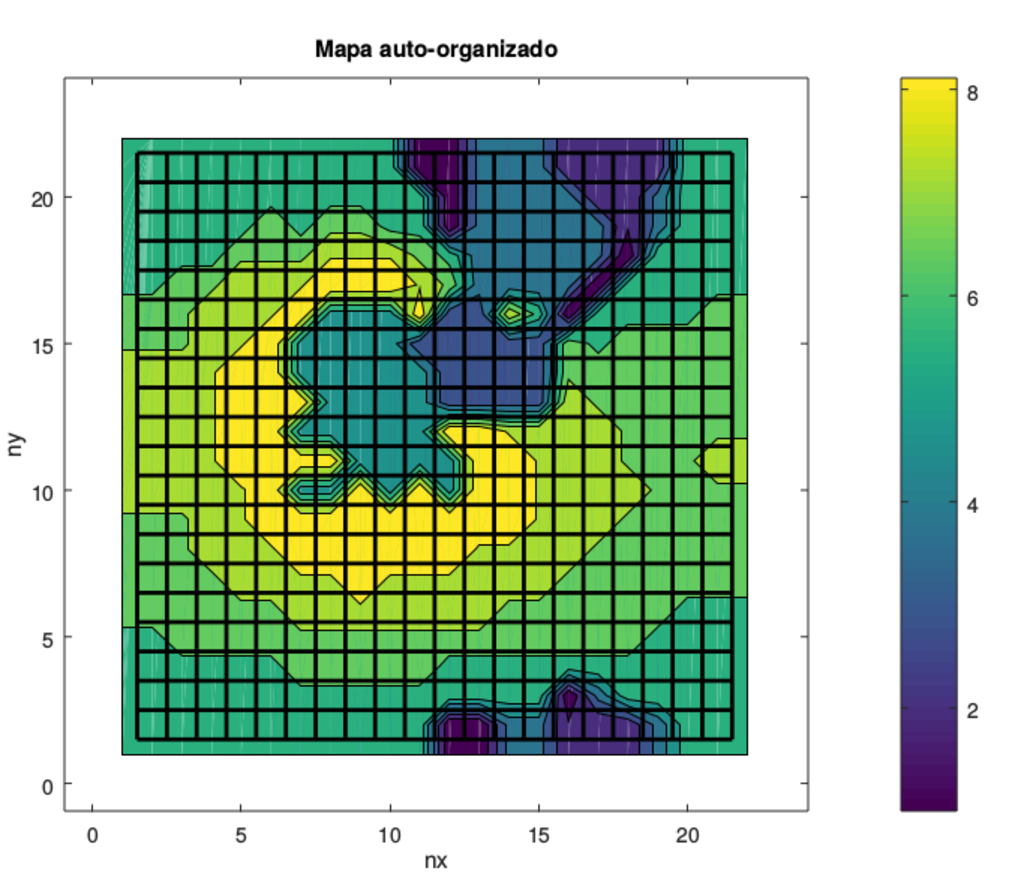
\includegraphics[width=7.0cm]{Imagens/SOM1000_2d.pdf}
\caption{Mapa auto-organizado (d) no milésimo ciclo de treinamento.}
\label{SOMd}
\end{figure}
\end{frame}

\begin{frame}
\frametitle{Treinamento}
\begin{figure}[H]
\centering
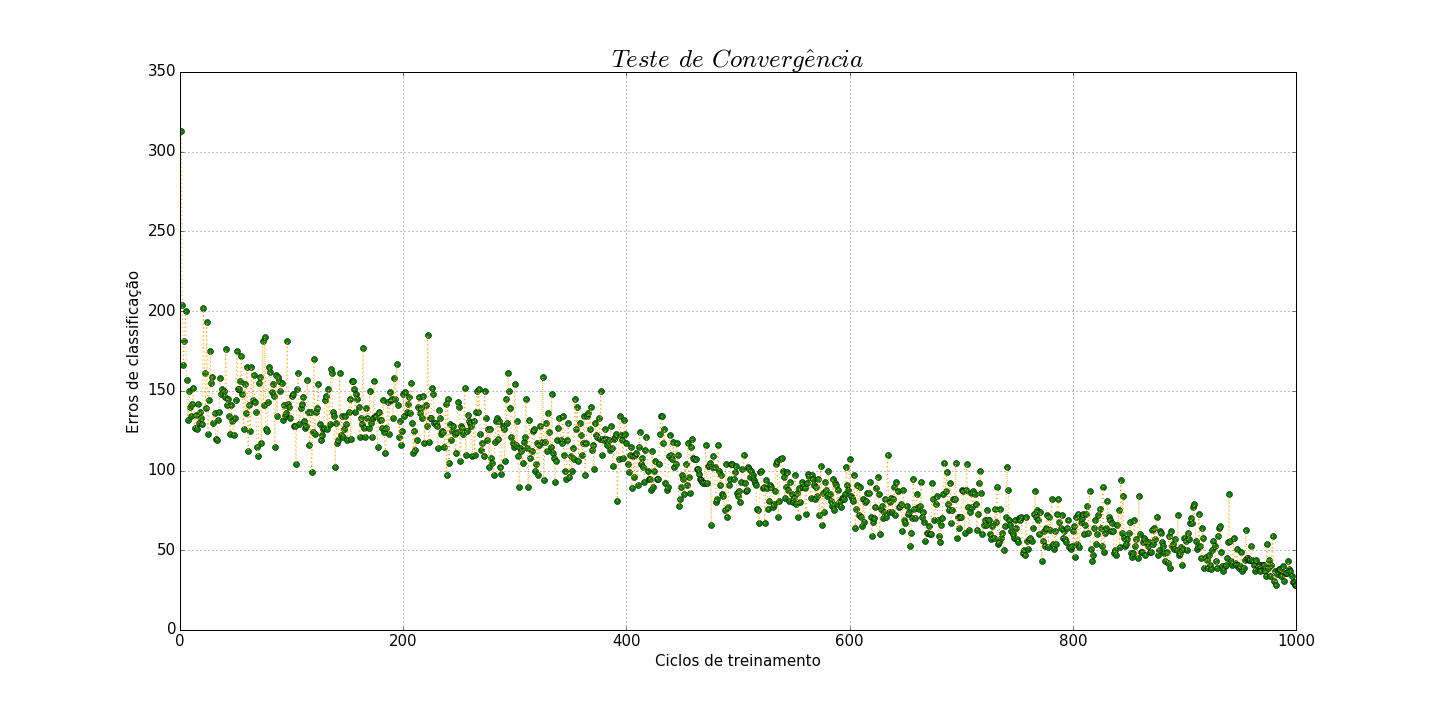
\includegraphics[scale=0.2]{Imagens/conv070917.png}
\caption{Teste de convergência da rede.}
\label{convergencia}
\end{figure} 
\end{frame}

%\subsection{Identificação}

\begin{frame}
\frametitle{Identificação}
\begin{figure}[H]
\centering
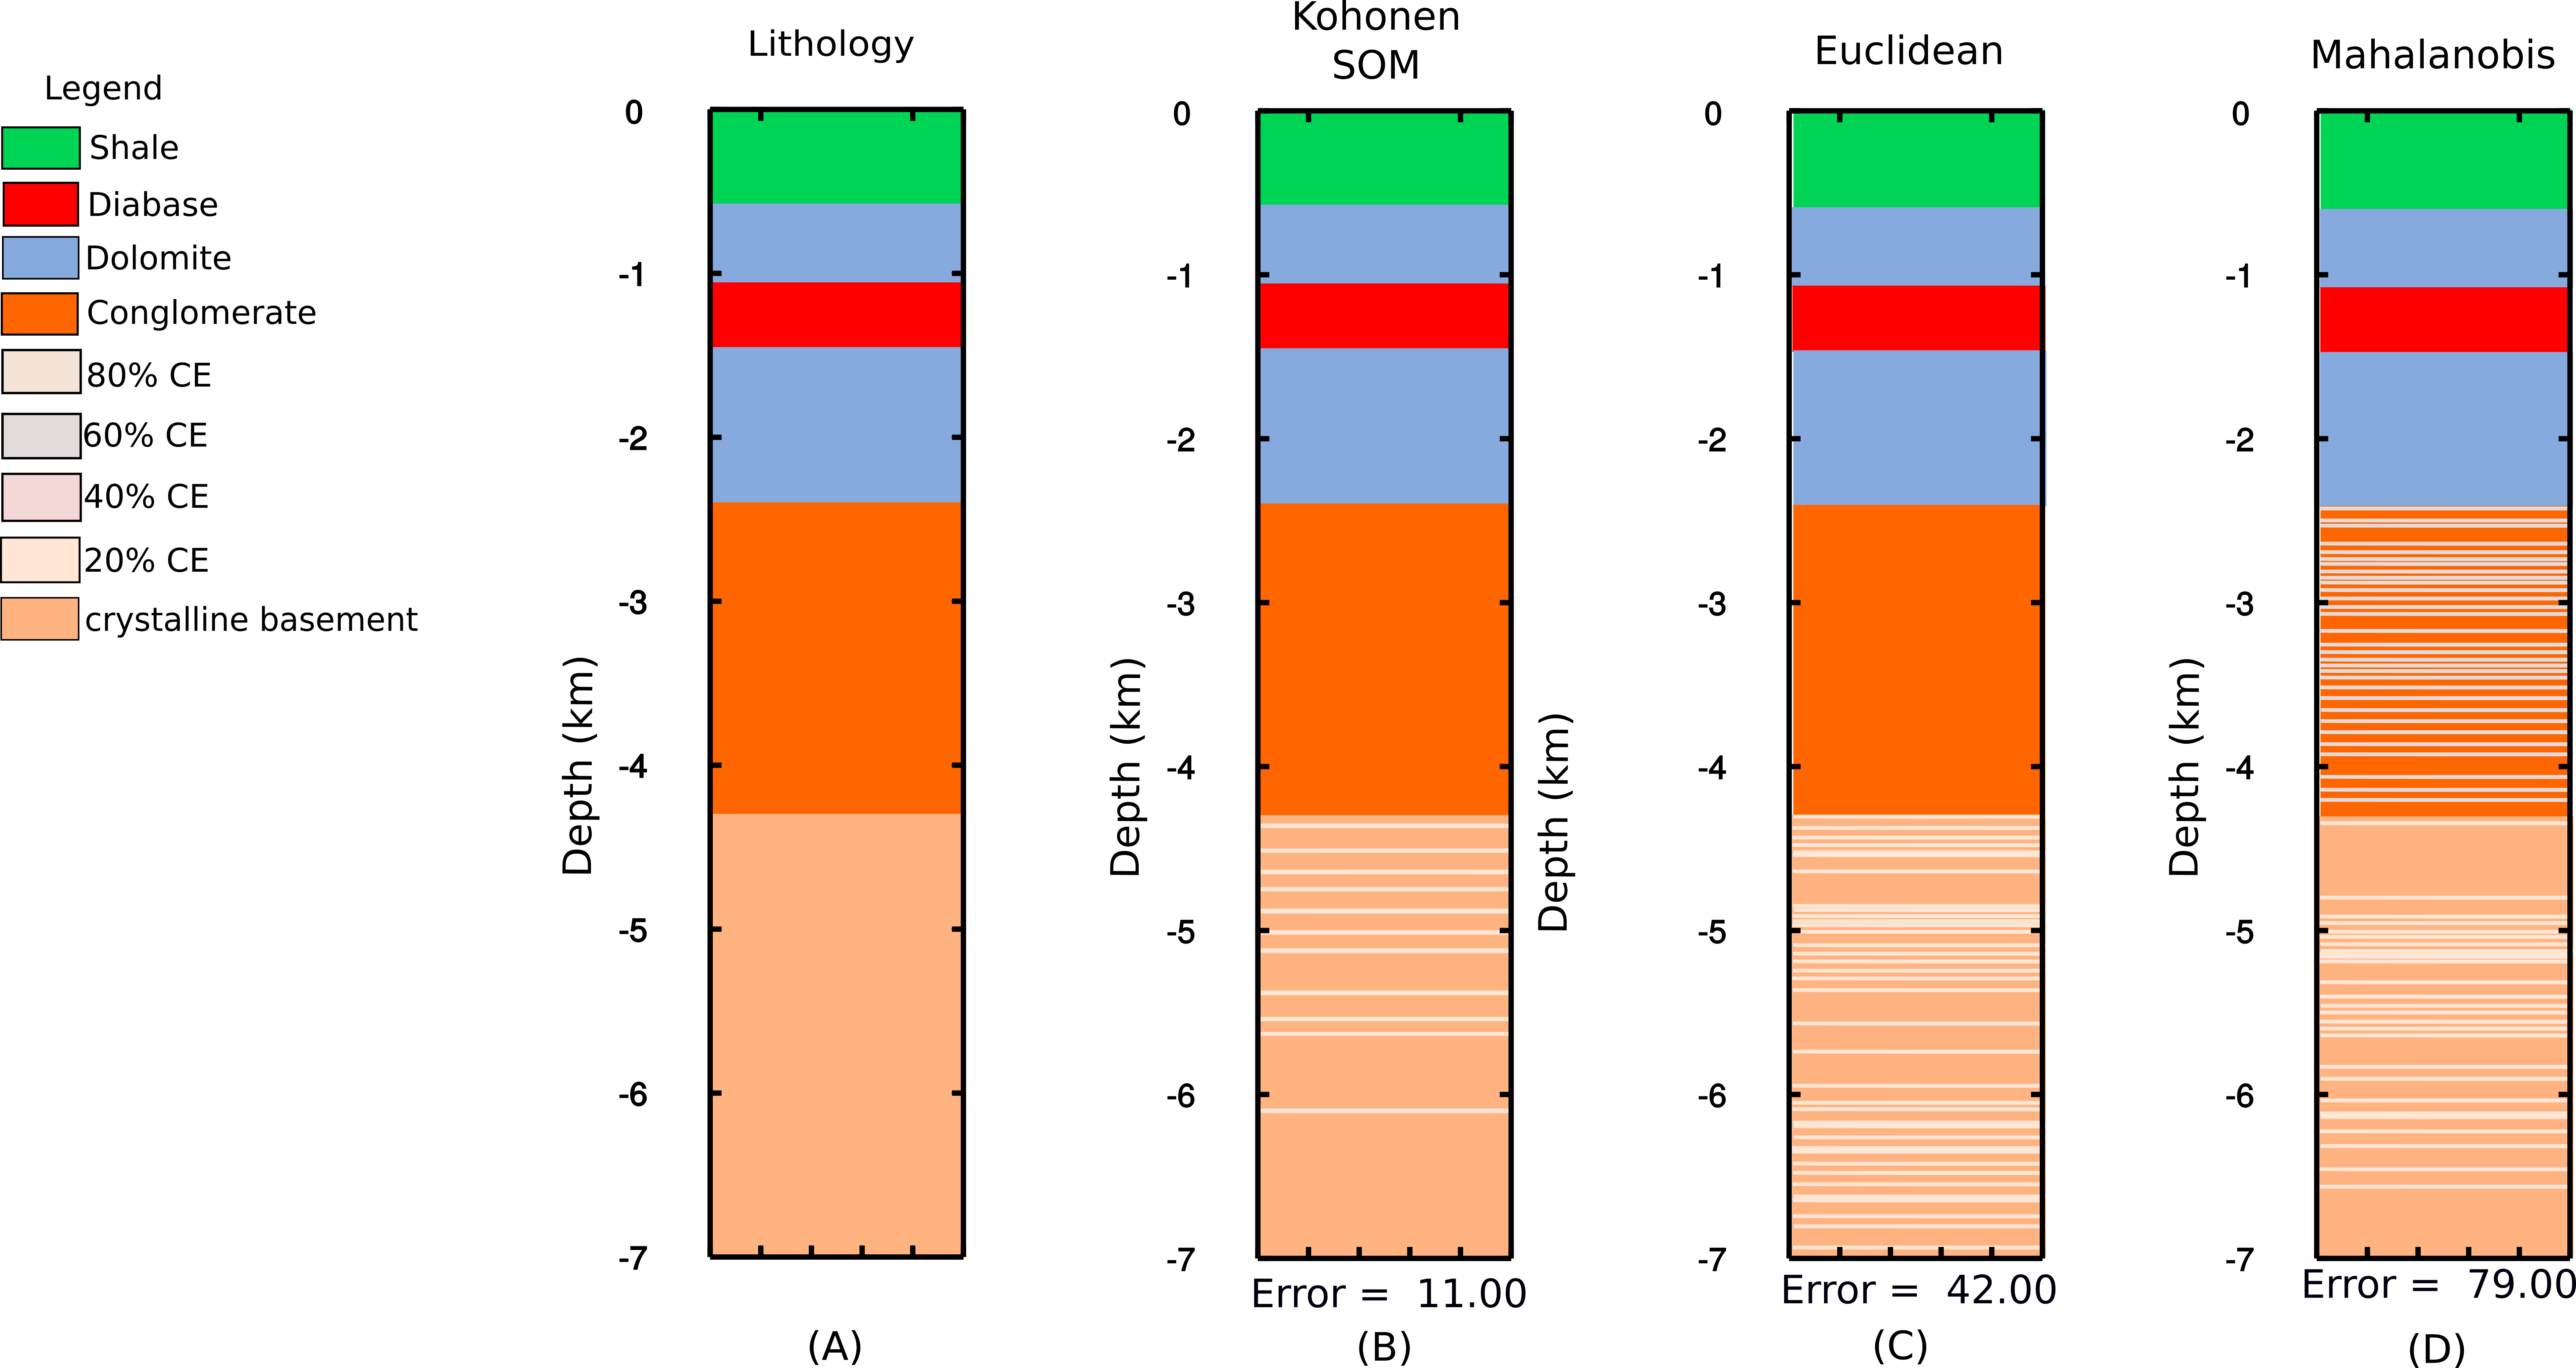
\includegraphics[scale=0.3]{Imagens/IDC1020118.png}
\caption{Dado de saída da rede para o poço de classificação C1.}
\label{Class C1}
\end{figure} 
\end{frame}

\begin{frame}
\frametitle{Identificação}
\begin{figure}[H]
\centering
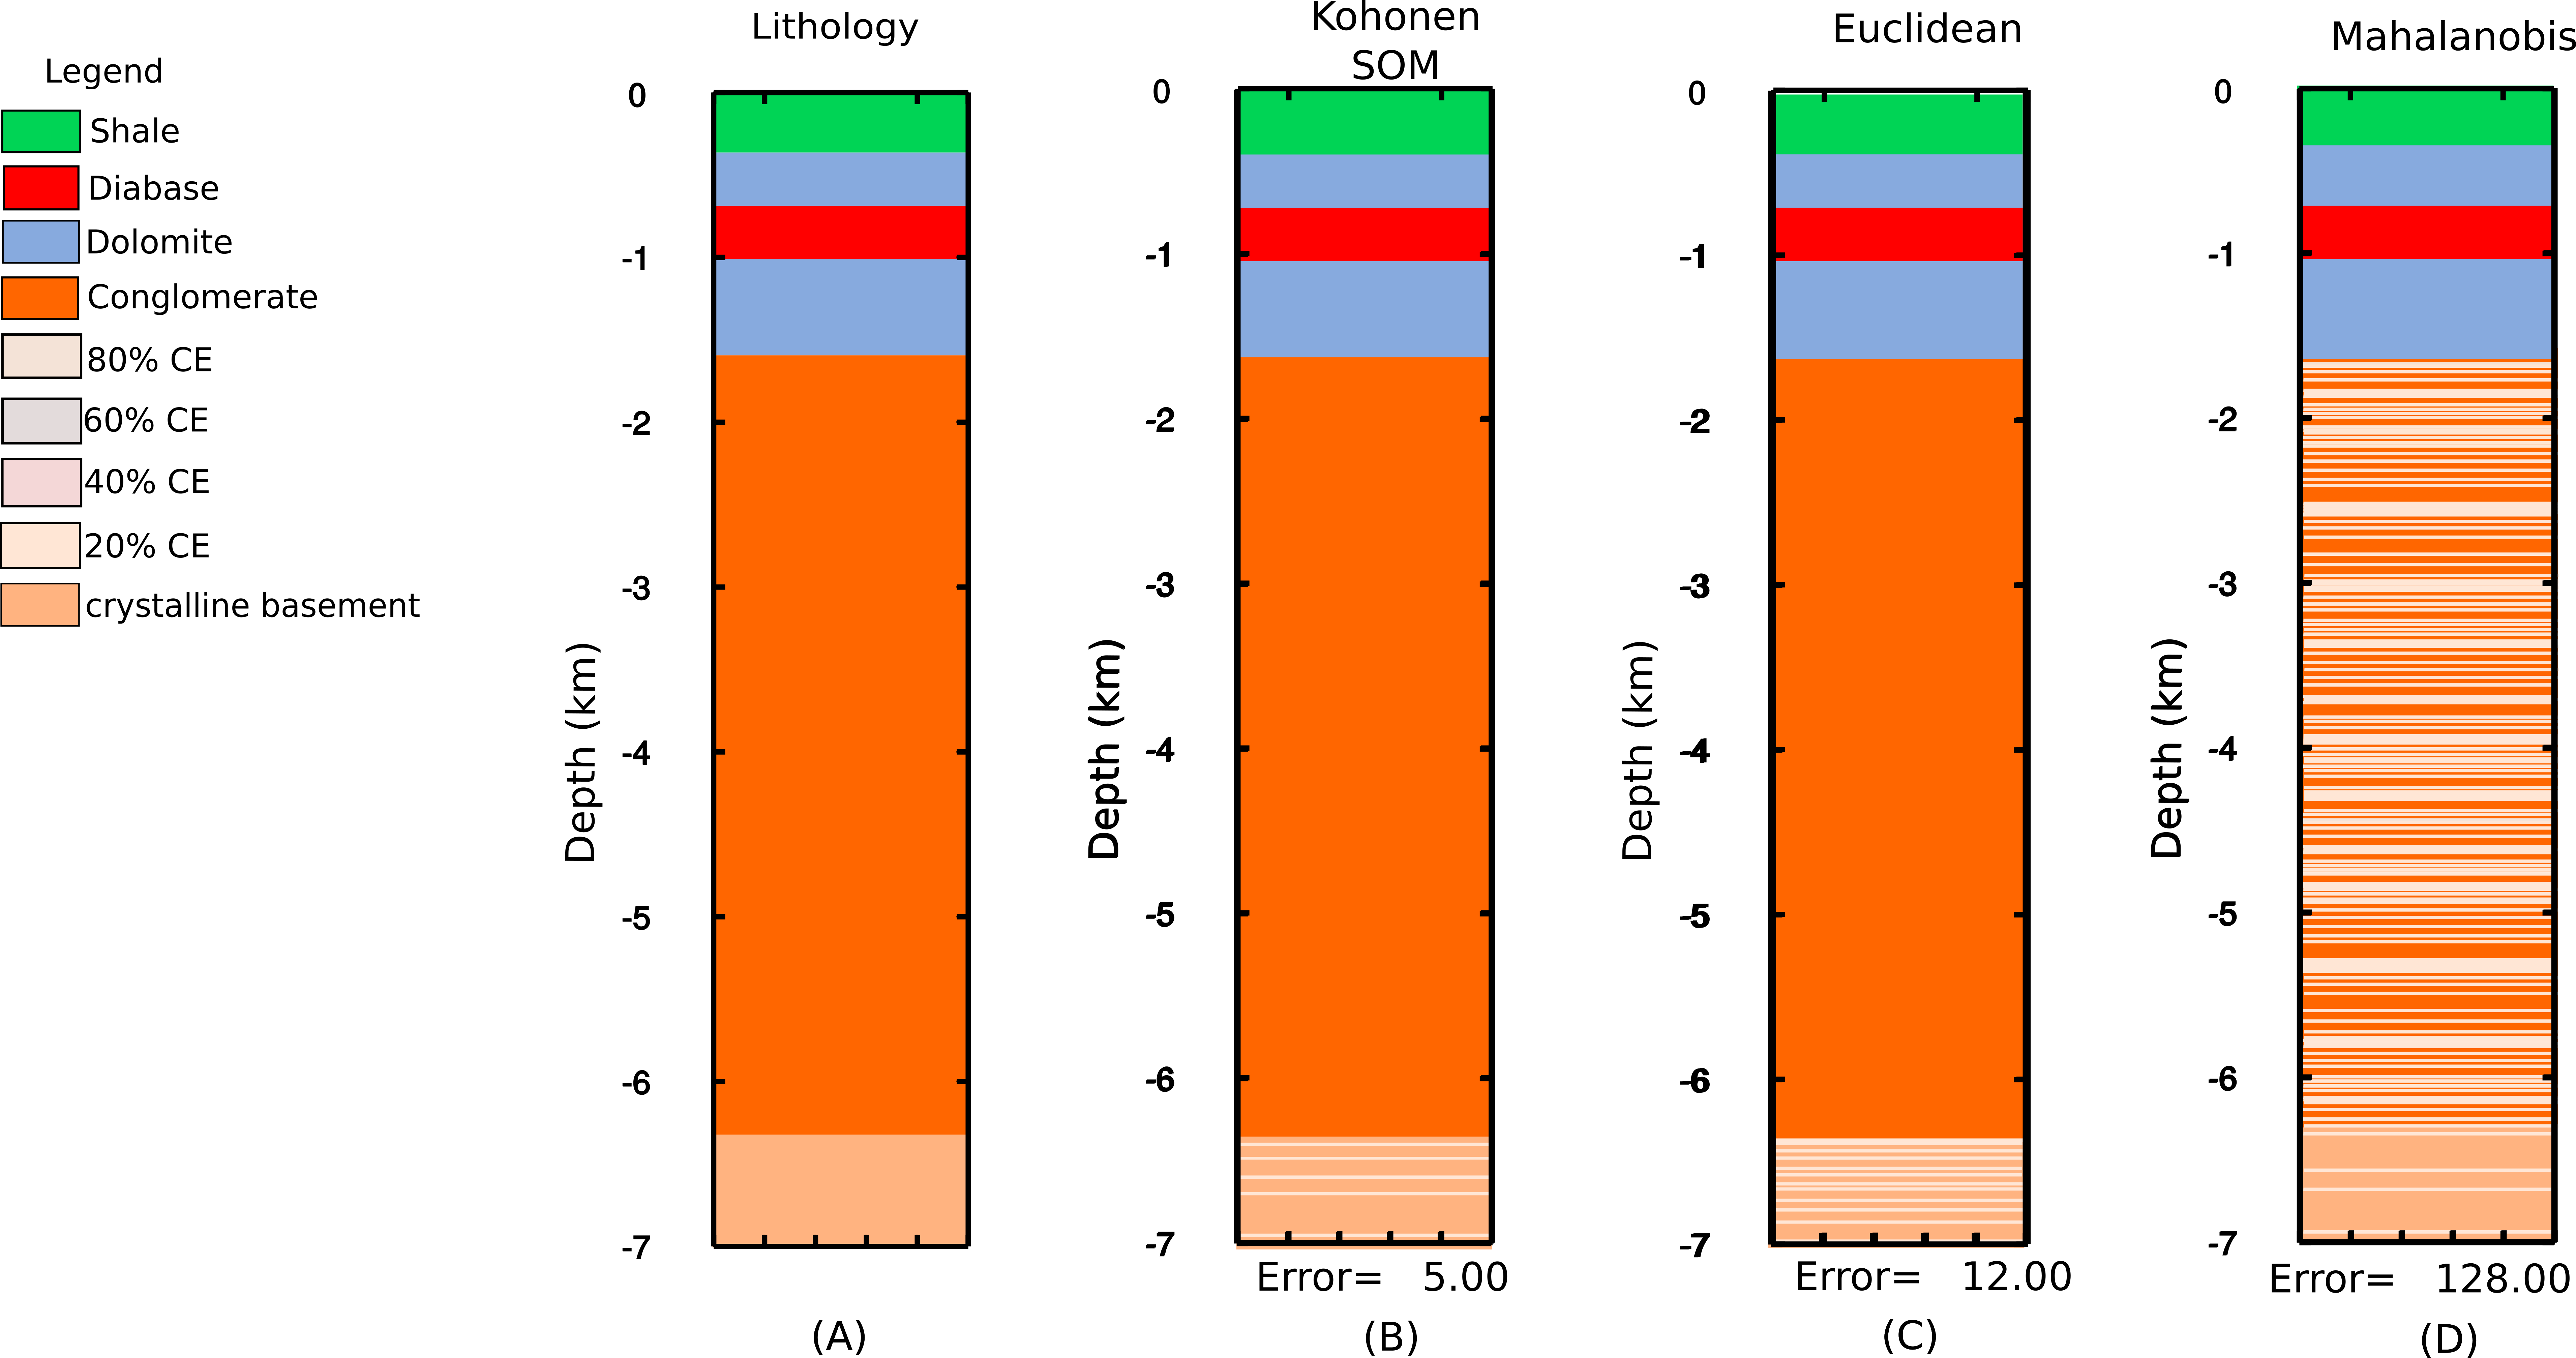
\includegraphics[scale=0.3]{Imagens/IDC2020118.png}
\caption{Dado de saída da rede para o poço de classificação C2.}
\label{Class C2}
\end{figure} 
\end{frame}

\begin{frame}
	\frametitle{Identificação}
\begin{table}[H]
	\centering
	\caption{}
	\label{Estatistica da rede}
	\begin{tabular}{@{}lcc@{}}
		\toprule
		\multicolumn{3}{c}{Estatística da Rede}         \\ \midrule
		Dados                       & Poço C1 & Poço C2 \\
		Dados de treinamento        & 697     & 697     \\
		Dados a serem classificados & 699     & 698     \\
		Neurônios da Rede           & 400     & 400     \\
		Neurônios vitoriosos        & 400     & 400     \\
		Neurônios sem uso           & 0       & 0       \\
		Erro                        & 11      & 5       \\ \bottomrule
	\end{tabular}
\end{table} 
\end{frame}

\subsection{Dado Real}

\begin{frame}
	\frametitle{Os dados reais}
	\begin{figure}[H]
		\centering
		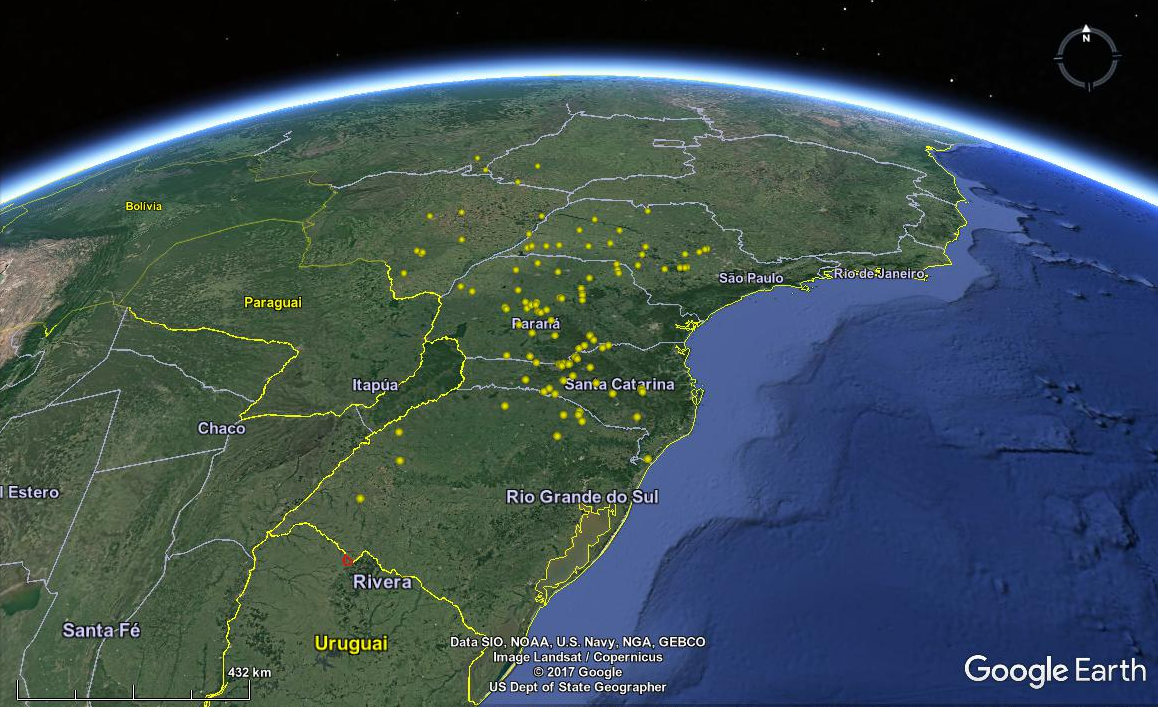
\includegraphics[scale=0.25]{Imagens/Pocos2.png}
		\caption{Localização dos poços de trabalho.}
		\label{real}
	\end{figure}
\end{frame}

\begin{frame}
	\frametitle{Os dados reais}
	\begin{enumerate}
		\item Os primeiros poços devem estar localizados próximos para garantir um controle inicial no que tange as litologias presentes no poço de treinamento. 
		\pause
		\item O poço de treinamento deve possuir a maior quantidade possível de dados por litologia
		\pause
		\item As entradas da rede devem ser compostas das mesmas propriedades físicas
		\pause
		\item Propriedades que definem litologia devem ser priorizadas quando possível.
	\end{enumerate}
\end{frame}

\begin{frame}
	\frametitle{Os dados reais}
	\begin{figure}[H]
		\centering
		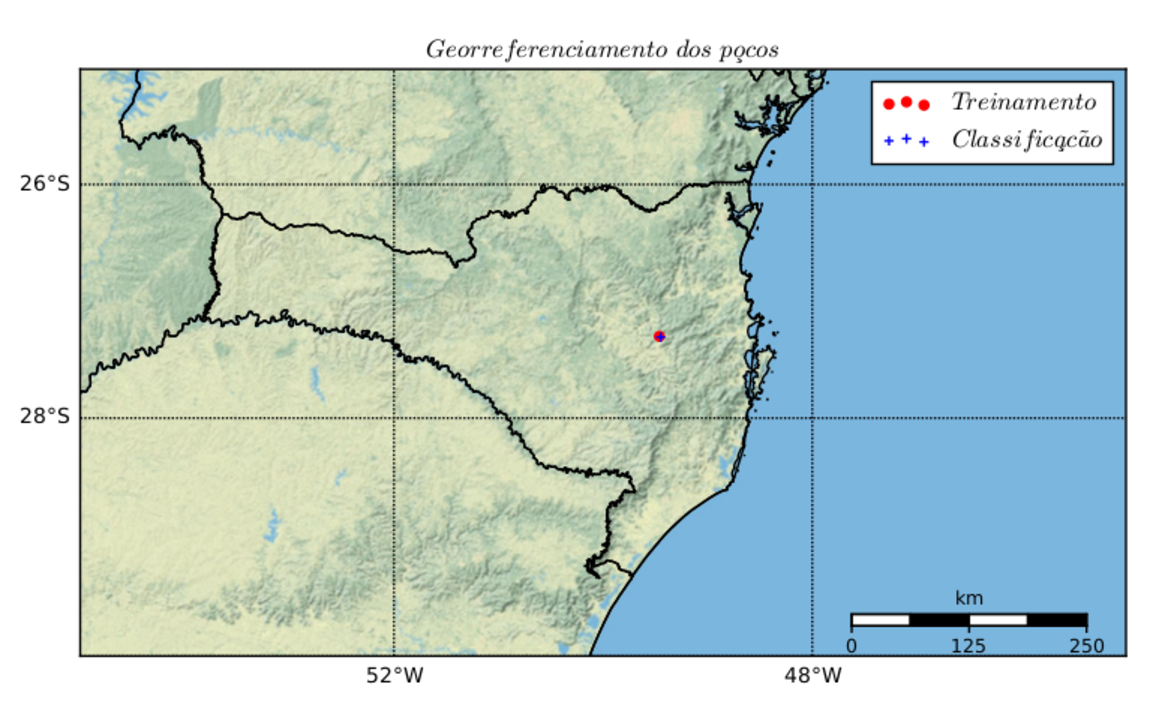
\includegraphics[scale=0.5]{Imagens/locmap02.pdf}
		\caption{Localização dos poços escolhidos.}
		\label{loc02}
	\end{figure}
\end{frame}

\begin{frame}
	\frametitle{Os dados reais: o poço de classificação}
	\begin{figure}[H]
		\centering
		\subfigure{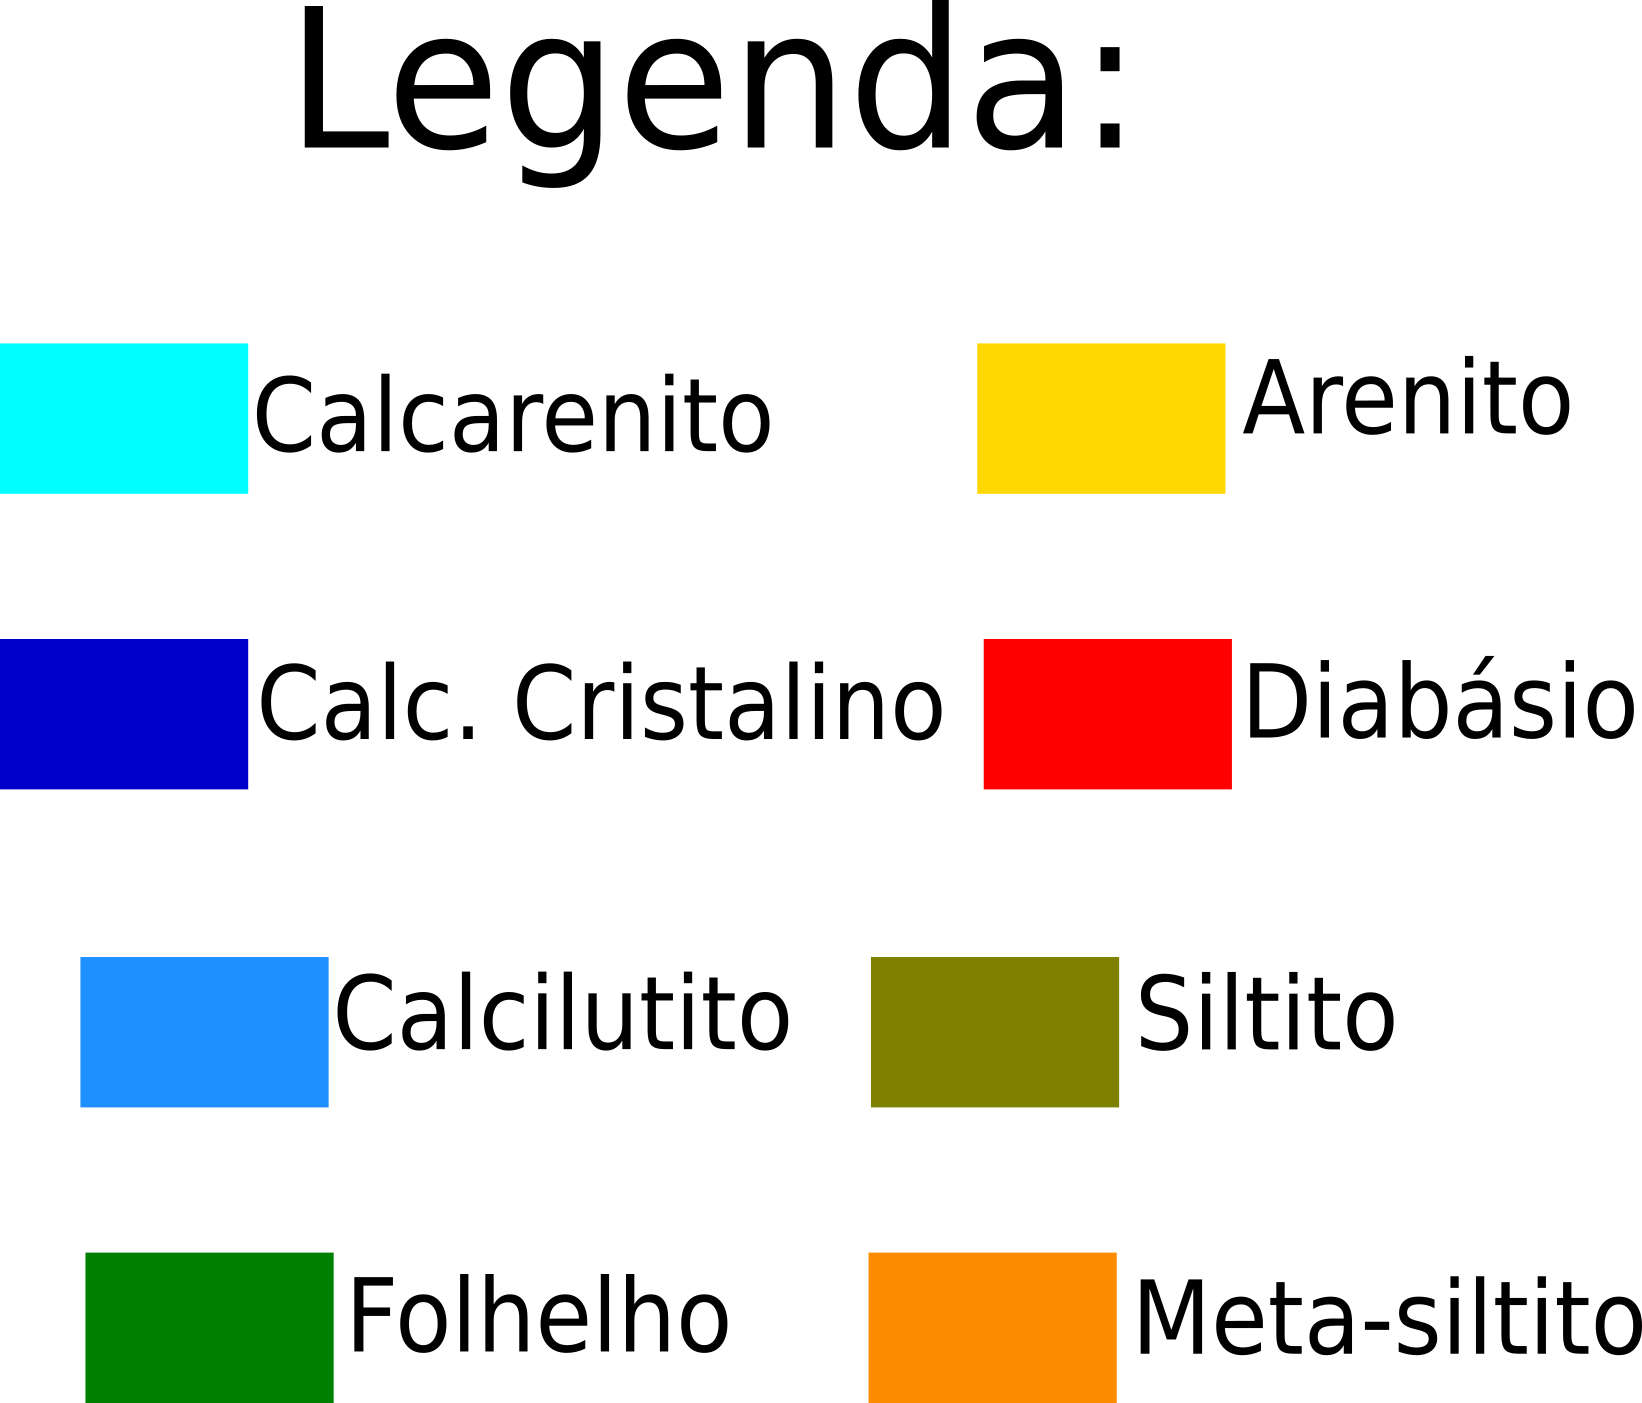
\includegraphics[width=1.3cm, height=1.3cm]{Imagens/legenda.png}}
		\qquad                                                           
		\subfigure[ref1][Litologia]{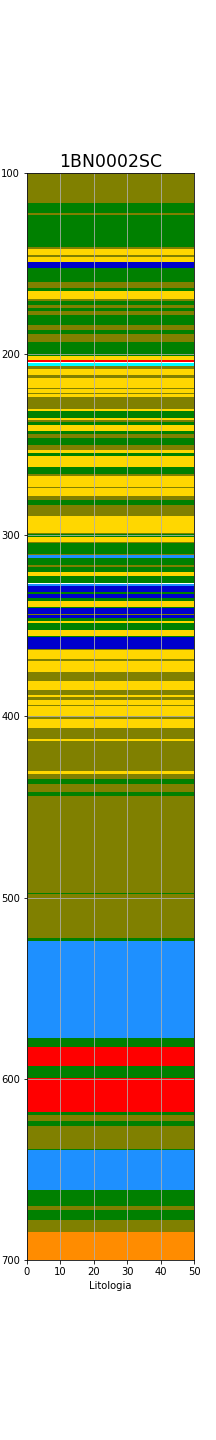
\includegraphics[width=1.9cm, height=8cm]{Imagens/1BN0002SC_lit2.png}}
		\qquad                                                             
		\subfigure[ref2][SP]{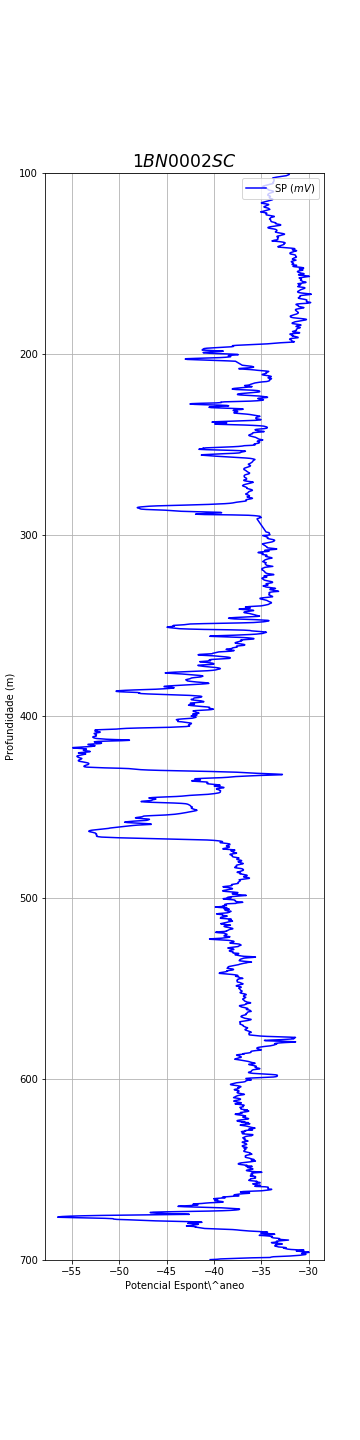
\includegraphics[width=2.0cm]{Imagens/1BN0002SC_SP.png}}
		\qquad
		\subfigure[ref3][RLAT]{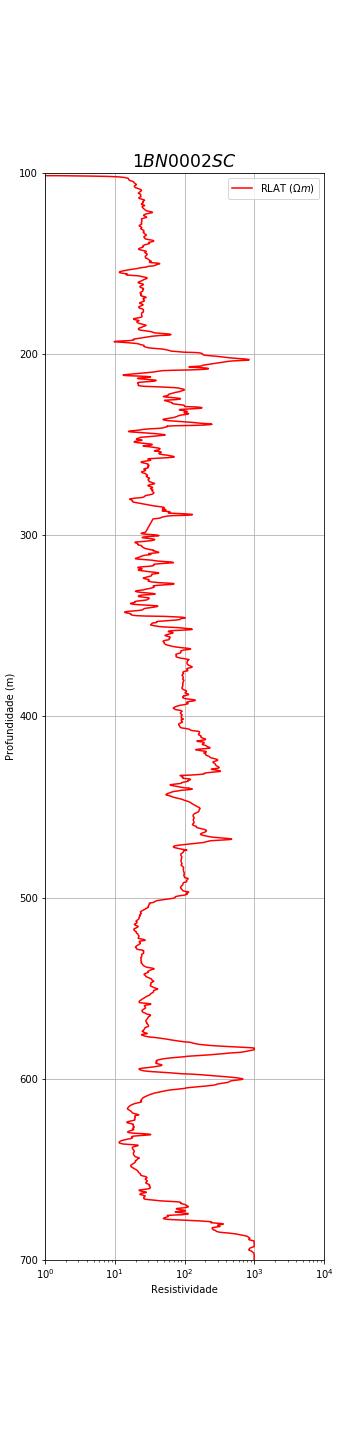
\includegraphics[width=2.0cm]{Imagens/1BN0002SC_res.png}}
		\qquad
		%\caption{Poço 1BN0002SC e as respectivas propriedades físicas escolhidas para o teste. Em (b) tem-se a variação de litologia com a profundidade, (c) o potencial espontâneo e em (d) a resistividade lateral.   } 
		\label{1BN0002SCa}
	\end{figure}
\end{frame}

\begin{frame}
	\frametitle{Os dados reais: o poço de classificação}
	\begin{figure}[H]
		\centering                                                         
		\subfigure{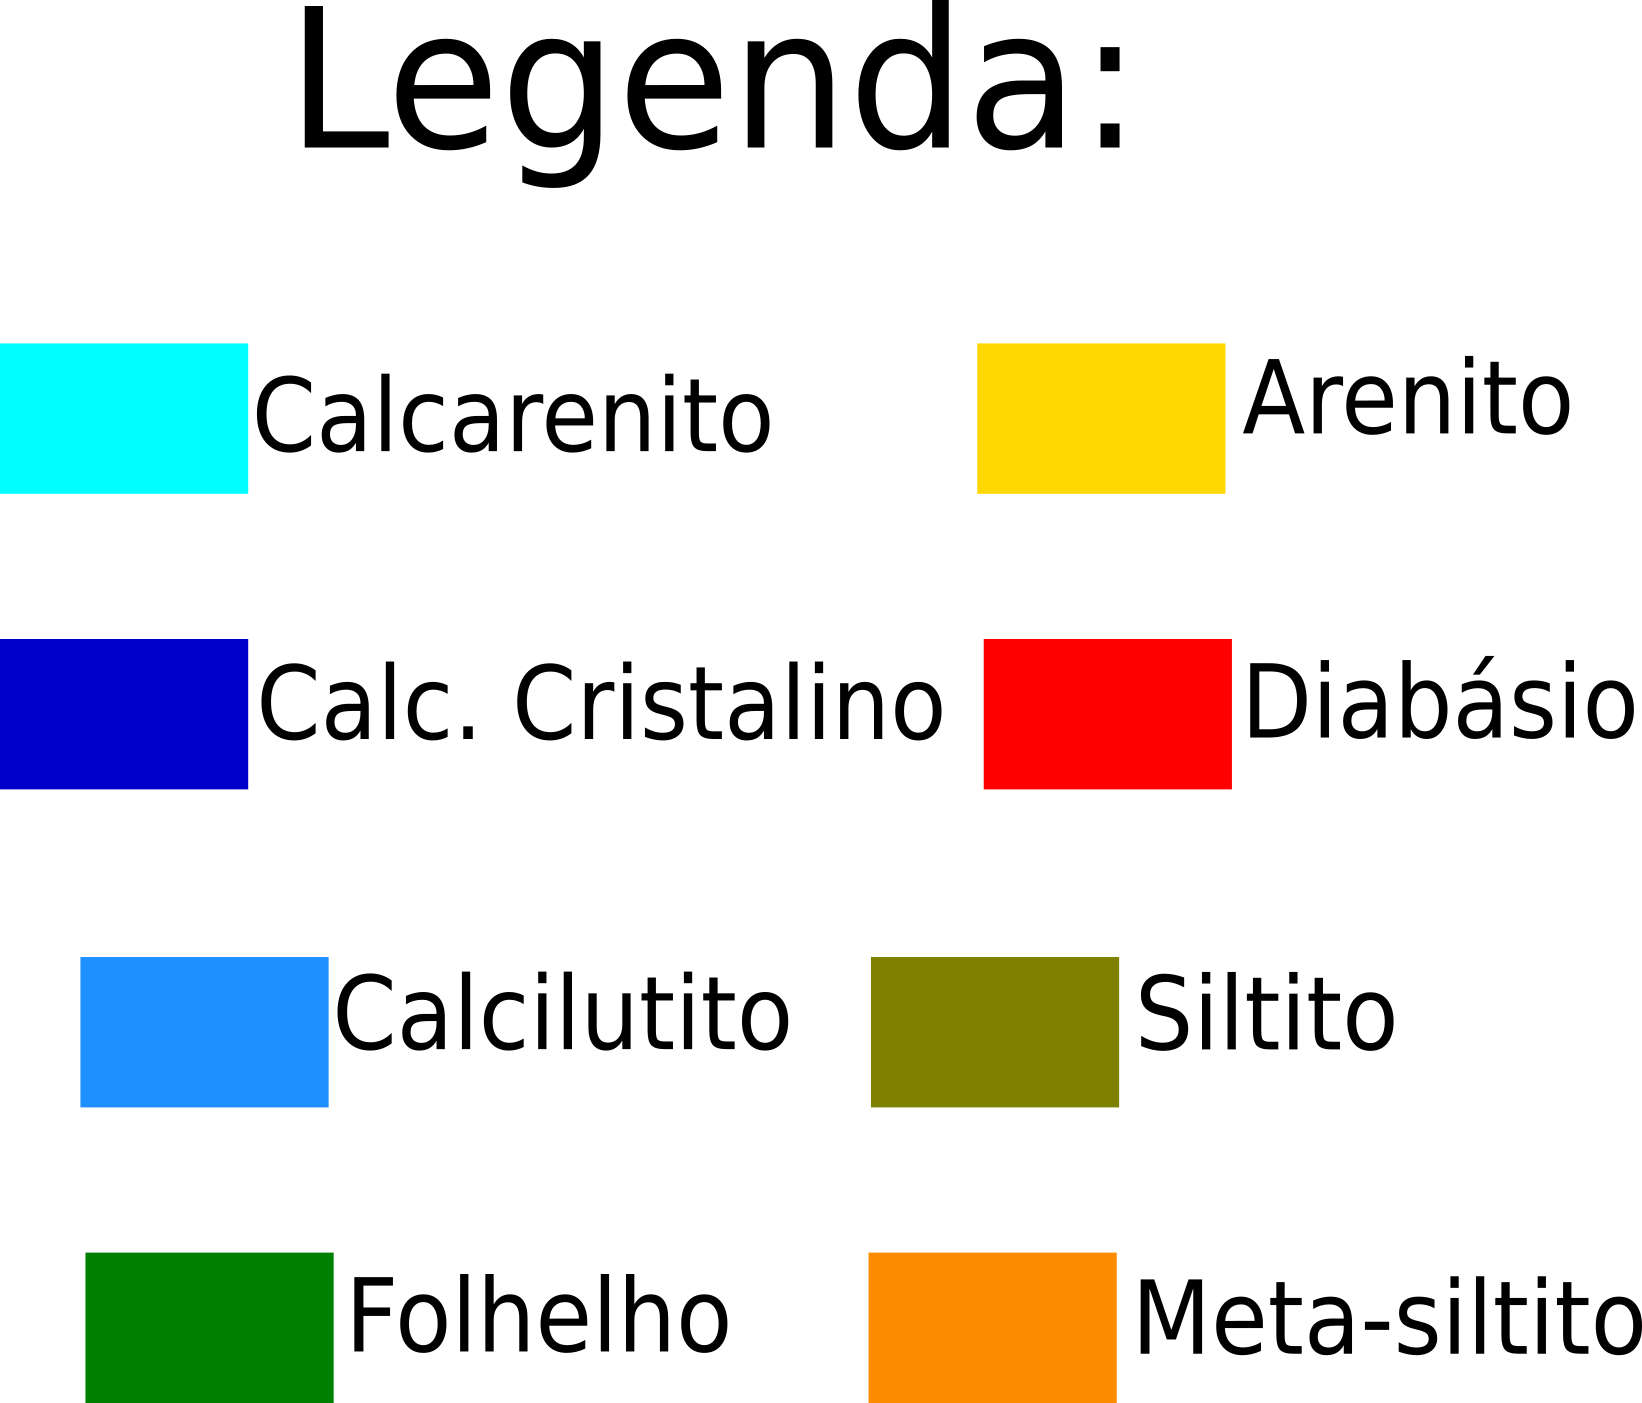
\includegraphics[width=1.3cm, height=1.3cm]{Imagens/legenda.png}}
		\qquad                                                           
		\subfigure[ref1][Litologia]{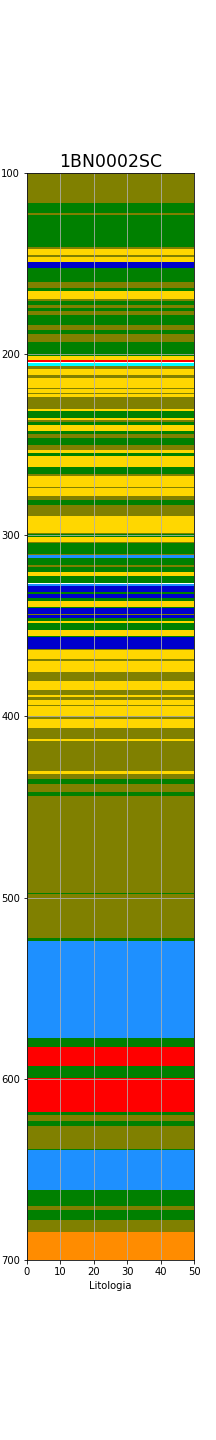
\includegraphics[width=1.9cm, height=8cm]{Imagens/1BN0002SC_lit2.png}}
		\qquad                                                             
		\subfigure[ref4][TTI]{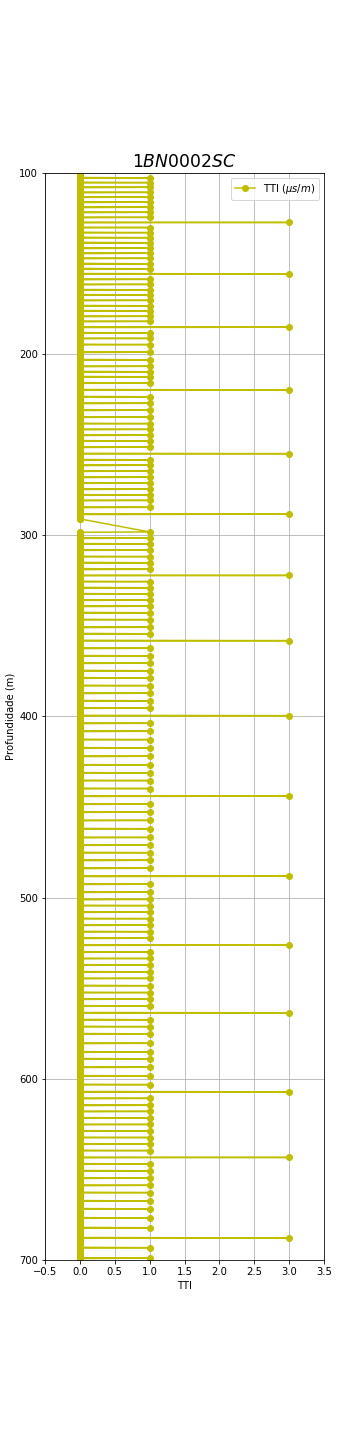
\includegraphics[width=2.0cm]{Imagens/1BN0002SC_TTI.png}}
		\qquad
		\subfigure[ref5][TOT]{\includegraphics[width=2.0cm]{Imagens/1BN0002SC_TOT.png}}
		\qquad
		%\caption{Poço 1BN0002SC e as respectivas propriedades físicas escolhidas para o teste. Em (b) tem-se a variação de litologia com a profundidade, (c) \textit{Transient Time Integrator} e em (d) TOT.}
		\label{1BN0002SCb}
	\end{figure}
\end{frame}

\begin{frame}
	\frametitle{Dado Real: teste 01}
	\begin{figure}[H]
		\centering
		\subfigure[ref1][Início]{\includegraphics[width=4.0cm]{Imagens/SOM1t01.pdf}}
		\qquad
		\subfigure[ref2][Metade]{\includegraphics[width=4.0cm]{Imagens/SOM2t01.pdf}}
		\qquad
		\subfigure[ref3][Final]{\includegraphics[width=4.0cm]{Imagens/SOM3t01.pdf}}
		\qquad
		%\caption{Mapas auto-organizáveis e sua evolução temporal. A figura (a) mostra a rede com $40$X$40$ neurônios no início do processo de treinamento. A figura (b) apresenta a rede no meio do processo de treinamento e (c) a rede no final do processo de treinamento.}
		\label{SOMt01}
	\end{figure}
\end{frame}


\begin{frame}
	\frametitle{Dado Real: teste 01}
	\begin{figure}[H]
		\centering
			\includegraphics[scale=0.2]{Imagens/conv01.png}
		%\caption{Convergência do teste $01$. Inicialmente a curva aproxima-se de uma função exponencial.}
		\label{Conv01}
	\end{figure} 
\end{frame}

\begin{frame}
	\frametitle{Dado Real: teste 02}
	\begin{figure}[H]
		\centering
		\subfigure[ref1][Início]{\includegraphics[width=4.0cm]{Imagens/SOM1t02.pdf}}
		\qquad
		\subfigure[ref2][Metade]{\includegraphics[width=4.0cm]{Imagens/SOM2t02.pdf}}
		\qquad
		\subfigure[ref3][Final]{\includegraphics[width=4.0cm]{Imagens/SOM3t02.pdf}}
		\qquad
		%\caption{Mapas auto-organizáveis e sua evolução temporal. A figura (a) mostra a rede com $40$X$40$ neurônios no início do processo de treinamento. A figura (b) apresenta a rede no meio do processo de treinamento e (c) a rede no final do processo de treinamento.}
		\label{SOMt02}
	\end{figure}
\end{frame}


\begin{frame}
	\frametitle{Dado Real: teste 02}
	\begin{figure}[H]
		\centering
		\includegraphics[scale=0.2]{Imagens/conv02.png}
		%\caption{Convergência do teste $02$. Inicialmente a curva aproxima-se de uma função exponencial.}
		\label{Conv02}
	\end{figure} 
\end{frame}

\begin{frame}
	\frametitle{Dado Real: teste 03}
	\begin{figure}[H]
		\centering
		\subfigure[ref1][Início]{\includegraphics[width=4.0cm]{Imagens/SOM1t03.pdf}}
		\qquad
		\subfigure[ref2][Metade]{\includegraphics[width=4.0cm]{Imagens/SOM2t03.pdf}}
		\qquad
		\subfigure[ref3][Final]{\includegraphics[width=4.0cm]{Imagens/SOM3t03.pdf}}
		\qquad
		%\caption{Mapas auto-organizáveis e sua evolução temporal. A figura (a) mostra a rede com $40$X$40$ neurônios no início do processo de treinamento. A figura (b) apresenta a rede no meio do processo de treinamento e (c) a rede no final do processo de treinamento.}
		\label{SOMt03}
	\end{figure}
\end{frame}


\begin{frame}
	\frametitle{Dado Real: teste 03}
	\begin{figure}[H]
		\centering
		\includegraphics[scale=0.2]{Imagens/conv03.png}
		%\caption{Convergência do teste $03$. Inicialmente a curva aproxima-se de uma função exponencial.}
		\label{Conv03}
	\end{figure} 
\end{frame}

\begin{frame}
	\frametitle{Dado Real: teste 04}
	\begin{figure}[H]
		\centering
		\subfigure[ref1][Início]{\includegraphics[width=4.0cm]{Imagens/SOM1t04.pdf}}
		\qquad
		\subfigure[ref2][Metade]{\includegraphics[width=4.0cm]{Imagens/SOM2t04.pdf}}
		\qquad
		\subfigure[ref3][Final]{\includegraphics[width=4.0cm]{Imagens/SOM3t04.pdf}}
		\qquad
		%\caption{Mapas auto-organizáveis e sua evolução temporal. A figura (a) mostra a rede com $40$X$40$ neurônios no início do processo de treinamento. A figura (b) apresenta a rede no meio do processo de treinamento e (c) a rede no final do processo de treinamento.}
		\label{SOMt04}
	\end{figure}
\end{frame}


\begin{frame}
	\frametitle{Dado Real: teste 04}
	\begin{figure}[H]
		\centering
		\includegraphics[scale=0.2]{Imagens/conv04.png}
		%\caption{Convergência do teste $04$. Inicialmente a curva aproxima-se de uma função exponencial.}
	\end{figure} 
\end{frame}

\begin{frame}
	\frametitle{Dado Real: teste 05}
	\begin{figure}[H]
		\centering
		\subfigure[ref1][Início]{\includegraphics[width=4.0cm]{Imagens/SOM1t05.pdf}}
		\qquad
		\subfigure[ref2][Metade]{\includegraphics[width=4.0cm]{Imagens/SOM2t05.pdf}}
		\qquad
		\subfigure[ref3][Final]{\includegraphics[width=4.0cm]{Imagens/SOM3t05.pdf}}
		\qquad
		%\caption{Mapas auto-organizáveis e sua evolução temporal. A figura (a) mostra a rede com $40$X$40$ neurônios no início do processo de treinamento. A figura (b) apresenta a rede no meio do processo de treinamento e (c) a rede no final do processo de treinamento.}
		\label{SOMt05}
	\end{figure}
\end{frame}


\begin{frame}
	\frametitle{Dado Real: teste 05}
	\begin{figure}[H]
		\centering
		\includegraphics[scale=0.2]{Imagens/conv05.png}
		%\caption{Convergência do teste $05$. Inicialmente a curva aproxima-se de uma função exponencial.}
		\label{Conv05}
	\end{figure} 
\end{frame}

\begin{frame}
	\frametitle{Dado Real: teste 06}
	\begin{figure}[H]
		\centering
		\subfigure[ref1][Início]{\includegraphics[width=4.0cm]{Imagens/SOM1t06.pdf}}
		\qquad
		\subfigure[ref2][Metade]{\includegraphics[width=4.0cm]{Imagens/SOM2t06.pdf}}
		\qquad
		\subfigure[ref3][Final]{\includegraphics[width=4.0cm]{Imagens/SOM3t06.pdf}}
		\qquad
		%\caption{Mapas auto-organizáveis e sua evolução temporal. A figura (a) mostra a rede com $40$X$40$ neurônios no início do processo de treinamento. A figura (b) apresenta a rede no meio do processo de treinamento e (c) a rede no final do processo de treinamento.}
		\label{SOMt06}
	\end{figure}
\end{frame}


\begin{frame}
	\frametitle{Dado Real: teste 06}
	\begin{figure}[H]
		\centering
		\includegraphics[scale=0.2]{Imagens/conv06.png}
		%\caption{Convergência do teste $06$. Inicialmente a curva aproxima-se de uma função exponencial.}
	\end{figure} 
\end{frame}

\begin{frame}
	\frametitle{Identificação do dado Real}
	\begin{table}[H]
		\centering
		\begin{tabular}{c|c}
			
			Litologia                    & Código numérico \\ % Note a separação de col. e a quebra de linhas
			\hline                                                             % para uma linha horizontal
			Calcilutito                   &  6              \\
			Calcarenito  		          &  8              \\
			Diabásio    	              &  65              \\
			Conglomerado                  &  42              \\
			Diamictito                    &  44              \\
			Arenito                       &  49              \\
			Siltito                       &  54              \\
			Folhelho                      &  57              \\
			Meta-siltito                  &  76              \\
			Calcário Cristalino           &  2              \\
			% não é preciso quebrar a última linha
			
		\end{tabular}
		\label{codigosreal}
		\caption{Tabela de referência para conversão do padrão numérico em litologia.}
	\end{table}
\end{frame}

\begin{frame}
	\frametitle{Identificação: teste 01}
	\begin{figure}[H]
		\centering
		\includegraphics[scale=0.18]{Imagens/result01.png}
	%	\caption{Identificação do teste 01. São apresentados dois gráficos. A esquerda encontra-se o resultado de classificação da rede e a direita o dado do poço original.}
		\label{IDt01}
	\end{figure} 
\end{frame}


\begin{frame}
	\frametitle{Identificação: teste 01}
	\begin{table}[H]
		\centering
		\caption{}
		\label{Estatistica do teste $01$}
		\begin{tabular}{@{}lc@{}}
			\toprule
			\multicolumn{2}{c}{Estatística do Teste $01$}         \\ \midrule
			Parâmetros                  & 1BN0002SC \\
			Época                       & 10       \\
			Erros                       & 2229       \\
			Neurônios da Rede           & 1600       \\
			Neurônios vitoriosos        & 976       \\
			Neurônios sem uso           & 624         \\
			Tempo de máquina            & 6,388 s   \\ \bottomrule
		\end{tabular}
	\end{table} 
\end{frame}

\begin{frame}
	\frametitle{Identificação: teste 02}
	\begin{figure}[H]
		\centering
		\includegraphics[scale=0.18]{Imagens/result02.png}
		%	\caption{Identificação do teste 01. São apresentados dois gráficos. A esquerda encontra-se o resultado de classificação da rede e a direita o dado do poço original.}
		\label{IDt02}
	\end{figure} 
\end{frame}


\begin{frame}
	\frametitle{Identificação: teste 02}
\begin{table}[H]
	\centering
	\caption{}
	\label{Estatistica do teste $02$}
	\begin{tabular}{@{}lc@{}}
		\toprule
		\multicolumn{2}{c}{Estatística do Teste $02$}         \\ \midrule
		Parâmetros                  & 1BN0002SC \\
		Época                       & 100       \\
		Erros                       & 2242       \\
		Neurônios da Rede           & 1600       \\
		Neurônios vitoriosos        & 1600       \\
		Neurônios sem uso           & 0         \\
		Tempo de máquina            & 62,01 s   \\ \bottomrule
	\end{tabular}
\end{table} 
\end{frame}

\begin{frame}
	\frametitle{Identificação: teste 03}
	\begin{figure}[H]
		\centering
		\includegraphics[scale=0.18]{Imagens/result03.png}
		%	\caption{Identificação do teste 01. São apresentados dois gráficos. A esquerda encontra-se o resultado de classificação da rede e a direita o dado do poço original.}
		\label{IDt03}
	\end{figure} 
\end{frame}


\begin{frame}
	\frametitle{Identificação: teste 03}
\begin{table}[H]
	\centering
	\caption{}
	\label{Estatistica do teste $03$}
	\begin{tabular}{@{}lc@{}}
		\toprule
		\multicolumn{2}{c}{Estatística do Teste $03$}         \\ \midrule
		Parâmetros                  & 1BN0002SC \\
		Época                       & 1000       \\
		Erros                       & 2226       \\
		Neurônios da Rede           & 1600       \\
		Neurônios vitoriosos        & 1600       \\
		Neurônios sem uso           & 0         \\
		Tempo de máquina            & 610,12 s   \\ \bottomrule
	\end{tabular}
\end{table} 
\end{frame}

\begin{frame}
	\frametitle{Identificação: teste 04}
	\begin{figure}[H]
		\centering
		\includegraphics[scale=0.18]{Imagens/result04.png}
		%	\caption{Identificação do teste 01. São apresentados dois gráficos. A esquerda encontra-se o resultado de classificação da rede e a direita o dado do poço original.}
		\label{IDt04}
	\end{figure} 
\end{frame}


\begin{frame}
	\frametitle{Identificação: teste 04}
\begin{table}[H]
	\centering
	\caption{}
	\label{Estatistica do teste $04$}
	\begin{tabular}{@{}lc@{}}
		\toprule
		\multicolumn{2}{c}{Estatística do Teste $04$}         \\ \midrule
		Parâmetros                  & 1BN0002SC \\
		Época                       & 10       \\
		Erros                       & 2219       \\
		Neurônios da Rede           & 400       \\
		Neurônios vitoriosos        & 400       \\
		Neurônios sem uso           & 0         \\
		Tempo de máquina            & 1,45 s   \\ \bottomrule
	\end{tabular}
\end{table} 
\end{frame}

\begin{frame}
	\frametitle{Identificação: teste 05}
	\begin{figure}[H]
		\centering
		\includegraphics[scale=0.18]{Imagens/result05.png}
		%	\caption{Identificação do teste 01. São apresentados dois gráficos. A esquerda encontra-se o resultado de classificação da rede e a direita o dado do poço original.}
		\label{IDt05}
	\end{figure} 
\end{frame}


\begin{frame}
	\frametitle{Identificação: teste 05}
\begin{table}[H]
	\centering
	\caption{}
	\label{Estatistica do teste $05$}
	\begin{tabular}{@{}lc@{}}
		\toprule
		\multicolumn{2}{c}{Estatística do Teste $05$}         \\ \midrule
		Parâmetros                  & 1BN0002SC \\
		Época                       & 100       \\
		Erros                       & 2408       \\
		Neurônios da Rede           & 400       \\
		Neurônios vitoriosos        & 400       \\
		Neurônios sem uso           & 0         \\
		Tempo de máquina            & 15,60 s   \\ \bottomrule
	\end{tabular}
\end{table} 
\end{frame}

\begin{frame}
	\frametitle{Identificação: teste 06}
	\begin{figure}[H]
		\centering
		\includegraphics[scale=0.18]{Imagens/result06.png}
		%	\caption{Identificação do teste 01. São apresentados dois gráficos. A esquerda encontra-se o resultado de classificação da rede e a direita o dado do poço original.}
	\end{figure} 
\end{frame}


\begin{frame}
	\frametitle{Identificação: teste 06}
\begin{table}[H]
	\centering
	\caption{}
	\label{Estatistica do teste $06$}
	\begin{tabular}{@{}lc@{}}
		\toprule
		\multicolumn{2}{c}{Estatística do Teste $06$}         \\ \midrule
		Parâmetros                  & 1BN0002SC \\
		Época                       & 1000       \\
		Erros                       & 2240       \\
		Neurônios da Rede           & 400       \\
		Neurônios vitoriosos        & 400       \\
		Neurônios sem uso           & 0         \\
		Tempo de máquina            & 153,82 s   \\ \bottomrule
	\end{tabular}
\end{table} 
\end{frame}

%%%%%%%%%%%%%%%%%%%%%%%%%%%%%%%%%%%%%%%%%%%%%%%%%%%%%%%%%%%%%%%%%%%%%%%%%%%%
%-------------------------CONCLUSÕES---------------------------------------
%%%%%%%%%%%%%%%%%%%%%%%%%%%%%%%%%%%%%%%%%%%%%%%%%%%%%%%%%%%%%%%%%%%%%%%%%%%%

\section{Conclusões}

\begin{frame}
\frametitle{Conclusões}

\begin{small}


	\begin{itemize}
		\footnotesize
		\item O algoritmo SOM superou os classificadores euclideanos e de Mahalanobis em um erro de $0.71\%$
		\pause
		\item A complexa distribuição dos agrupamentos no espaço de atributos levou a erros da ordem de $18.28\%$ (Mahalanobis) e $1.71\%$ (Euclides), no melhor cenário (poço C$2$ ).
		\pause
		\item Os classificadores não conseguem identificar corretamente o padrão sino no dado de poço. 
		\pause
		\item O classificador euclideano consegue identificar o padrão caixa ao contrário do classificador de Mahalanobis.
		\pause
		\item A rede neuronal de Kohonen SOM apresentou melhor desempenho no que tange a identificação de mistura de rochas como o padrão sino.
		\pause
		\item As baixas performances médias registradas para os seis testes com dados reais apresentaram erros de $2230$ amostras uma performance de $75\%$ . É possível que tal desempenho esteja relacionado a dois principais fatores.
		\pause
		\begin{enumerate}
			\footnotesize
			\item As propriedades físicas escolhidas para o treinamento da rede.
			\pause
			\item A inexistência de um banco com dados que contemplem as propriedades físicas e unidades litológicas do poço a ser analisado.
		\end{enumerate}
		
	\end{itemize}

\end{small}	
\end{frame}

\section{Próximas etapas}

\begin{frame}
	\frametitle{Próximas etapas}
	
	\begin{small}
		\begin{itemize}
			\item Reavaliação das propriedades físicas utilizadas.
			\pause
			\item Priorizar as curvas de Raios Gama, Densidade, Neutrão e Resistividade.
			\pause
			\item Criação do Banco de dados das propriedades físicas.
			\pause
			\item Estudar outras relações de vizinhanças dentro da rede neuronal
			\pause
			\item Submeter o primeiro artigo
			\pause
			\item Qualificar
			\end{itemize}
	\end{small}	
\end{frame}


%%%%%%%%%%%%%%%%%%%%%%%%%%%%%%%%%%%%%%%%%%%%%%%%%%%%%%%%%%%%%%%%%%%%%%%%%%%%
%-------------------------CRONOGRAMA---------------------------------------
%%%%%%%%%%%%%%%%%%%%%%%%%%%%%%%%%%%%%%%%%%%%%%%%%%%%%%%%%%%%%%%%%%%%%%%%%%%%

\section{Cronograma}		
\begin{frame}
\begin{table}[H]
%	\centering
	\flushleft
	
	% definindo o tamanho da fonte para small
	% outros possíveis tamanhos: footnotesize, scriptsize
	\begin{scriptsize}
		
		% redefinindo o espaçamento das colunas
		\setlength{\tabcolsep}{.5pt}
		
		% \cline é semelhante ao \hline, porém é possível indicar as colunas que terão essa a linha horizontal
		% \multicolumn{10}{c|}{Meses} indica que dez colunas serão mescladas e a palavra Meses estará centralizada dentro delas.
		\rotatebox{0}{
			\begin{tabular}{|c|c|c|c|c|c|c|c|c|c|c|c|c|c|c|c|c|c|c|c|c|c|c|c|c|}\hline
				& \multicolumn{24}{c|}{Meses}\\ \cline{2-25}
				\raisebox{1.5ex}{Etapa} & 01 & 02 & 03 & 04 & 05 & 06 & 07 & 08 & 09 & 10 & 11 & 12 & 13 & 14 & 15 & 16 & 17 & 18 & 19 & 20 & \textcolor{red}{21} & 22 & 23 & 24 \\ \hline	
				Pesquisa na Literatura     & X & X & X & X & X & X & X & X & X& X & X & X & X & X & X & X & X & X & X & X & \textcolor{red}{X} & X & X & X\\ \hline
				Disciplinas                        & & & X & X & X & X & X & X &  X & X & X & X & & & X & X & X & X & X & X & \textcolor{red}{X} & X & X & X \\ \hline
				Formulação da Rede        & & & & & & & & X &  X & X & X & X & X & X & X & X & & & & & & & & \\ \hline
				Treino                               & & & & & & & & & & & & & X & X & X & X & X & X & X & X & \textcolor{red}{X} & X & X & X \\ \hline
				Resultado                         & & & & & & & & & & & & & & & & & & & & X & \textcolor{red}{X} & X & X & X \\ \hline
				Artigo 1                            & & & & & & & & & & & & & & & & & & & & & & & X & X \\ \hline
				Artigo 2                            & & & & & & & & & & & & & & & & & & & & & & & & \\ \hline
				Tese                                  & & & & & & & & & & & & & & & & & & & & & & & & \\ \hline
			\end{tabular}
		}
	\end{scriptsize}
	\caption{Cronograma das atividades previstas para o primeiro biênio. Em  {\color{red}vermelho} encontra-se o mês de setembro de 2018.}
	\label{t1_cronograma}
\end{table}

\end{frame}


\begin{frame}
\begin{table}[H]
\centering

% definindo o tamanho da fonte para small
% outros possíveis tamanhos: footnotesize, scriptsize
\begin{scriptsize}

% redefinindo o espaçamento das colunas
\setlength{\tabcolsep}{.5pt}

% \cline é semelhante ao \hline, porém é possível indicar as colunas que terão essa a linha horizontal
% \multicolumn{10}{c|}{Meses} indica que dez colunas serão mescladas e a palavra Meses estará centralizada dentro delas.
\rotatebox{0}{
\begin{tabular}{|c|c|c|c|c|c|c|c|c|c|c|c|c|c|c|c|c|c|c|c|c|c|c|c|c|}\hline
& \multicolumn{24}{c|}{Meses}\\ \cline{2-25}
\raisebox{1.5ex}{Etapa} & 25 & 26 & 27 & 28 & 29 & 30 & 31 & 32 & 33 & 34 & 35 & 36 & 37 & 38 & 39 & 40 & 41 & 42 & 43 & 44 & 45 & 46 & 47 & 48 \\ \hline

Pesquisa na Literatura & X & X & X & X & X & X & & & & & & & & & & & & & & & & & & \\ \hline
Disciplinas & & & & & & & & & & & & & & & & & & & & & & & & \\ \hline
Formulação da Rede & & & & & & & & & & & & & & & & & & & & & & & & \\ \hline
Treino & & & & & & & & & & & & & & & & & & & & & & & & \\ \hline
Resultado & & X & X & X & X & X & X & X & & & & & & & & & & & & & & & & \\ \hline
Artigo 1 &X & X & X & X &X & X& X& & & & & & & & & & & & & & & & & \\ \hline
Artigo 2 & & & & & X & X & X & X & X &X & X& X& X& X& X& X& X& & & & & & & \\ \hline
Tese & & & & & & & & & & & & & X&X & X & X & X & X & X & X & X & & & \\ \hline

\end{tabular}
}
\end{scriptsize}
\caption{Cronograma das atividades previstas para o segundo biênio.}
\label{t2_cronograma}
\end{table}

\end{frame}	



\begin{frame}[allowframebreaks]
\frametitle{Referencias}
%\beamertemplatetextbibitems
\tiny
\bibliographystyle{apalike}
\bibliography{references}
\end{frame}

\makeatother
{
\begin{frame}
	%\titlepage
	\begin{figure}
		\includegraphics[scale=0.25]{Imagens/logonvertical.jpg}
	\end{figure}
	\begin{center}
		\begin{minipage}{0.77\textwidth}
			\small
			\begin{center}
				Rua General José Cristino, 77 CEP 20921-400\\
				Rua General Bruce, 586 CEP 20921-030\\
				Bairro Imperial de São Cristóvão, Rio de Janeiro - RJ\\
				PABX: 55 21 3504-9100\\
				\url{www.on.br}
			\end{center}
		\end{minipage}
	\end{center}
\end{frame}
}



\end{document}